\documentclass[twoside]{book}

% Packages required by doxygen
\usepackage{fixltx2e}
\usepackage{calc}
\usepackage{doxygen}
\usepackage[export]{adjustbox} % also loads graphicx
\usepackage{graphicx}
\usepackage[utf8]{inputenc}
\usepackage{makeidx}
\usepackage{multicol}
\usepackage{multirow}
\PassOptionsToPackage{warn}{textcomp}
\usepackage{textcomp}
\usepackage[nointegrals]{wasysym}
\usepackage[table]{xcolor}

% Font selection
\usepackage[T1]{fontenc}
\usepackage[scaled=.90]{helvet}
\usepackage{courier}
\usepackage{amssymb}
\usepackage{sectsty}
\renewcommand{\familydefault}{\sfdefault}
\allsectionsfont{%
  \fontseries{bc}\selectfont%
  \color{darkgray}%
}
\renewcommand{\DoxyLabelFont}{%
  \fontseries{bc}\selectfont%
  \color{darkgray}%
}
\newcommand{\+}{\discretionary{\mbox{\scriptsize$\hookleftarrow$}}{}{}}

% Page & text layout
\usepackage{geometry}
\geometry{%
  a4paper,%
  top=2.5cm,%
  bottom=2.5cm,%
  left=2.5cm,%
  right=2.5cm%
}
\tolerance=750
\hfuzz=15pt
\hbadness=750
\setlength{\emergencystretch}{15pt}
\setlength{\parindent}{0cm}
\setlength{\parskip}{3ex plus 2ex minus 2ex}
\makeatletter
\renewcommand{\paragraph}{%
  \@startsection{paragraph}{4}{0ex}{-1.0ex}{1.0ex}{%
    \normalfont\normalsize\bfseries\SS@parafont%
  }%
}
\renewcommand{\subparagraph}{%
  \@startsection{subparagraph}{5}{0ex}{-1.0ex}{1.0ex}{%
    \normalfont\normalsize\bfseries\SS@subparafont%
  }%
}
\makeatother

% Headers & footers
\usepackage{fancyhdr}
\pagestyle{fancyplain}
\fancyhead[LE]{\fancyplain{}{\bfseries\thepage}}
\fancyhead[CE]{\fancyplain{}{}}
\fancyhead[RE]{\fancyplain{}{\bfseries\leftmark}}
\fancyhead[LO]{\fancyplain{}{\bfseries\rightmark}}
\fancyhead[CO]{\fancyplain{}{}}
\fancyhead[RO]{\fancyplain{}{\bfseries\thepage}}
\fancyfoot[LE]{\fancyplain{}{}}
\fancyfoot[CE]{\fancyplain{}{}}
\fancyfoot[RE]{\fancyplain{}{\bfseries\scriptsize Generated by Doxygen }}
\fancyfoot[LO]{\fancyplain{}{\bfseries\scriptsize Generated by Doxygen }}
\fancyfoot[CO]{\fancyplain{}{}}
\fancyfoot[RO]{\fancyplain{}{}}
\renewcommand{\footrulewidth}{0.4pt}
\renewcommand{\chaptermark}[1]{%
  \markboth{#1}{}%
}
\renewcommand{\sectionmark}[1]{%
  \markright{\thesection\ #1}%
}

% Indices & bibliography
\usepackage{natbib}
\usepackage[titles]{tocloft}
\setcounter{tocdepth}{3}
\setcounter{secnumdepth}{5}
\makeindex

% Hyperlinks (required, but should be loaded last)
\usepackage{ifpdf}
\ifpdf
  \usepackage[pdftex,pagebackref=true]{hyperref}
\else
  \usepackage[ps2pdf,pagebackref=true]{hyperref}
\fi
\hypersetup{%
  colorlinks=true,%
  linkcolor=blue,%
  citecolor=blue,%
  unicode%
}

% Custom commands
\newcommand{\clearemptydoublepage}{%
  \newpage{\pagestyle{empty}\cleardoublepage}%
}

\usepackage{caption}
\captionsetup{labelsep=space,justification=centering,font={bf},singlelinecheck=off,skip=4pt,position=top}

%===== C O N T E N T S =====

\begin{document}

% Titlepage & ToC
\hypersetup{pageanchor=false,
             bookmarksnumbered=true,
             pdfencoding=unicode
            }
\pagenumbering{roman}
\begin{titlepage}
\vspace*{7cm}
\begin{center}%
{\Large Blood\+Transfusion }\\
\vspace*{1cm}
{\large Generated by Doxygen 1.8.11}\\
\end{center}
\end{titlepage}
\clearemptydoublepage
\tableofcontents
\clearemptydoublepage
\pagenumbering{arabic}
\hypersetup{pageanchor=true}

%--- Begin generated contents ---
\chapter{Module Index}
\section{Modules}
Here is a list of all modules\+:\begin{DoxyCompactList}
\item \contentsline{section}{O\+M\+H\+\_\+\+Commands}{\pageref{group___o_m_h___commands}}{}
\end{DoxyCompactList}

\chapter{Namespace Index}
\section{Packages}
Here are the packages with brief descriptions (if available)\+:\begin{DoxyCompactList}
\item\contentsline{section}{\hyperlink{namespace_b83}{B83} }{\pageref{namespace_b83}}{}
\item\contentsline{section}{\hyperlink{namespace_b83_1_1_logic_expression_parser}{B83.\+Logic\+Expression\+Parser} }{\pageref{namespace_b83_1_1_logic_expression_parser}}{}
\item\contentsline{section}{\hyperlink{namespace_little_brain}{Little\+Brain} }{\pageref{namespace_little_brain}}{}
\item\contentsline{section}{\hyperlink{namespace_little_brain_1_1_g_m_addr}{Little\+Brain.\+G\+M\+Addr} }{\pageref{namespace_little_brain_1_1_g_m_addr}}{}
\item\contentsline{section}{\hyperlink{namespace_unity_template_projects}{Unity\+Template\+Projects} }{\pageref{namespace_unity_template_projects}}{}
\end{DoxyCompactList}

\chapter{Hierarchical Index}
\section{Class Hierarchy}
This inheritance list is sorted roughly, but not completely, alphabetically\+:\begin{DoxyCompactList}
\item \contentsline{section}{Command\+Sequence}{\pageref{class_command_sequence}}{}
\item \contentsline{section}{Little\+Brain.\+G\+M\+Addr.\+Command\+Sequence}{\pageref{class_little_brain_1_1_g_m_addr_1_1_command_sequence}}{}
\item Exception\begin{DoxyCompactList}
\item \contentsline{section}{B83.\+Logic\+Expression\+Parser.\+Parse\+Exception}{\pageref{class_b83_1_1_logic_expression_parser_1_1_parse_exception}}{}
\end{DoxyCompactList}
\item \contentsline{section}{B83.\+Logic\+Expression\+Parser.\+Expression\+Context}{\pageref{class_b83_1_1_logic_expression_parser_1_1_expression_context}}{}
\item \contentsline{section}{Expression\+Parser}{\pageref{class_expression_parser}}{}
\item \contentsline{section}{Little\+Brain.\+G\+M\+Addr.\+Expression\+Parser}{\pageref{class_little_brain_1_1_g_m_addr_1_1_expression_parser}}{}
\item \contentsline{section}{Expression\+Parser\+DT}{\pageref{class_expression_parser_d_t}}{}
\item \contentsline{section}{B83.\+Logic\+Expression\+Parser.\+I\+Command\+Parser}{\pageref{interface_b83_1_1_logic_expression_parser_1_1_i_command_parser}}{}
\item \contentsline{section}{B83.\+Logic\+Expression\+Parser.\+I\+Logic\+Result}{\pageref{interface_b83_1_1_logic_expression_parser_1_1_i_logic_result}}{}
\begin{DoxyCompactList}
\item \contentsline{section}{B83.\+Logic\+Expression\+Parser.\+Combine\+And}{\pageref{class_b83_1_1_logic_expression_parser_1_1_combine_and}}{}
\item \contentsline{section}{B83.\+Logic\+Expression\+Parser.\+Combine\+Not}{\pageref{class_b83_1_1_logic_expression_parser_1_1_combine_not}}{}
\item \contentsline{section}{B83.\+Logic\+Expression\+Parser.\+Combine\+Or}{\pageref{class_b83_1_1_logic_expression_parser_1_1_combine_or}}{}
\item \contentsline{section}{B83.\+Logic\+Expression\+Parser.\+Combine\+Xor}{\pageref{class_b83_1_1_logic_expression_parser_1_1_combine_xor}}{}
\item \contentsline{section}{B83.\+Logic\+Expression\+Parser.\+Compare\+Statement}{\pageref{class_b83_1_1_logic_expression_parser_1_1_compare_statement}}{}
\begin{DoxyCompactList}
\item \contentsline{section}{B83.\+Logic\+Expression\+Parser.\+Compare\+Equal}{\pageref{class_b83_1_1_logic_expression_parser_1_1_compare_equal}}{}
\item \contentsline{section}{B83.\+Logic\+Expression\+Parser.\+Compare\+Greater}{\pageref{class_b83_1_1_logic_expression_parser_1_1_compare_greater}}{}
\item \contentsline{section}{B83.\+Logic\+Expression\+Parser.\+Compare\+Greater\+Or\+Equal}{\pageref{class_b83_1_1_logic_expression_parser_1_1_compare_greater_or_equal}}{}
\item \contentsline{section}{B83.\+Logic\+Expression\+Parser.\+Compare\+Lower}{\pageref{class_b83_1_1_logic_expression_parser_1_1_compare_lower}}{}
\item \contentsline{section}{B83.\+Logic\+Expression\+Parser.\+Compare\+Lower\+Or\+Equal}{\pageref{class_b83_1_1_logic_expression_parser_1_1_compare_lower_or_equal}}{}
\item \contentsline{section}{B83.\+Logic\+Expression\+Parser.\+Compare\+Not\+Equal}{\pageref{class_b83_1_1_logic_expression_parser_1_1_compare_not_equal}}{}
\end{DoxyCompactList}
\item \contentsline{section}{B83.\+Logic\+Expression\+Parser.\+Constant\+Bool}{\pageref{class_b83_1_1_logic_expression_parser_1_1_constant_bool}}{}
\item \contentsline{section}{B83.\+Logic\+Expression\+Parser.\+Delegate\+Bool}{\pageref{class_b83_1_1_logic_expression_parser_1_1_delegate_bool}}{}
\item \contentsline{section}{B83.\+Logic\+Expression\+Parser.\+Logic\+Expression}{\pageref{class_b83_1_1_logic_expression_parser_1_1_logic_expression}}{}
\item \contentsline{section}{B83.\+Logic\+Expression\+Parser.\+Number\+To\+Bool}{\pageref{class_b83_1_1_logic_expression_parser_1_1_number_to_bool}}{}
\item \contentsline{section}{B83.\+Logic\+Expression\+Parser.\+Value\+Provider}{\pageref{class_b83_1_1_logic_expression_parser_1_1_value_provider}}{}
\begin{DoxyCompactList}
\item \contentsline{section}{B83.\+Logic\+Expression\+Parser.\+Expression\+Variable}{\pageref{class_b83_1_1_logic_expression_parser_1_1_expression_variable}}{}
\end{DoxyCompactList}
\end{DoxyCompactList}
\item \contentsline{section}{B83.\+Logic\+Expression\+Parser.\+I\+Number\+Provider}{\pageref{interface_b83_1_1_logic_expression_parser_1_1_i_number_provider}}{}
\begin{DoxyCompactList}
\item \contentsline{section}{B83.\+Logic\+Expression\+Parser.\+Bool\+To\+Number}{\pageref{class_b83_1_1_logic_expression_parser_1_1_bool_to_number}}{}
\item \contentsline{section}{B83.\+Logic\+Expression\+Parser.\+Constant\+Number}{\pageref{class_b83_1_1_logic_expression_parser_1_1_constant_number}}{}
\item \contentsline{section}{B83.\+Logic\+Expression\+Parser.\+Custom\+Function}{\pageref{class_b83_1_1_logic_expression_parser_1_1_custom_function}}{}
\item \contentsline{section}{B83.\+Logic\+Expression\+Parser.\+Delegate\+Number}{\pageref{class_b83_1_1_logic_expression_parser_1_1_delegate_number}}{}
\item \contentsline{section}{B83.\+Logic\+Expression\+Parser.\+Number\+Expression}{\pageref{class_b83_1_1_logic_expression_parser_1_1_number_expression}}{}
\item \contentsline{section}{B83.\+Logic\+Expression\+Parser.\+Operation\+Add}{\pageref{class_b83_1_1_logic_expression_parser_1_1_operation_add}}{}
\item \contentsline{section}{B83.\+Logic\+Expression\+Parser.\+Operation\+Negate}{\pageref{class_b83_1_1_logic_expression_parser_1_1_operation_negate}}{}
\item \contentsline{section}{B83.\+Logic\+Expression\+Parser.\+Operation\+Power}{\pageref{class_b83_1_1_logic_expression_parser_1_1_operation_power}}{}
\item \contentsline{section}{B83.\+Logic\+Expression\+Parser.\+Operation\+Product}{\pageref{class_b83_1_1_logic_expression_parser_1_1_operation_product}}{}
\item \contentsline{section}{B83.\+Logic\+Expression\+Parser.\+Operation\+Reciprocal}{\pageref{class_b83_1_1_logic_expression_parser_1_1_operation_reciprocal}}{}
\item \contentsline{section}{B83.\+Logic\+Expression\+Parser.\+Parameter\+List}{\pageref{class_b83_1_1_logic_expression_parser_1_1_parameter_list}}{}
\item \contentsline{section}{B83.\+Logic\+Expression\+Parser.\+Value\+Provider}{\pageref{class_b83_1_1_logic_expression_parser_1_1_value_provider}}{}
\end{DoxyCompactList}
\item I\+Pointer\+Click\+Handler\begin{DoxyCompactList}
\item \contentsline{section}{Message\+Handler\+Base}{\pageref{class_message_handler_base}}{}
\item \contentsline{section}{Object\+Message\+Handler\+Base}{\pageref{class_object_message_handler_base}}{}
\begin{DoxyCompactList}
\item \contentsline{section}{Object\+Message\+Handler}{\pageref{class_object_message_handler}}{}
\end{DoxyCompactList}
\end{DoxyCompactList}
\item \contentsline{section}{B83.\+Logic\+Expression\+Parser.\+I\+String\+Provider}{\pageref{interface_b83_1_1_logic_expression_parser_1_1_i_string_provider}}{}
\begin{DoxyCompactList}
\item \contentsline{section}{B83.\+Logic\+Expression\+Parser.\+Compare\+Statement}{\pageref{class_b83_1_1_logic_expression_parser_1_1_compare_statement}}{}
\item \contentsline{section}{B83.\+Logic\+Expression\+Parser.\+Constant\+String}{\pageref{class_b83_1_1_logic_expression_parser_1_1_constant_string}}{}
\item \contentsline{section}{B83.\+Logic\+Expression\+Parser.\+Custom\+String\+Function}{\pageref{class_b83_1_1_logic_expression_parser_1_1_custom_string_function}}{}
\item \contentsline{section}{B83.\+Logic\+Expression\+Parser.\+Delegate\+String}{\pageref{class_b83_1_1_logic_expression_parser_1_1_delegate_string}}{}
\item \contentsline{section}{B83.\+Logic\+Expression\+Parser.\+Operation\+Concat}{\pageref{class_b83_1_1_logic_expression_parser_1_1_operation_concat}}{}
\item \contentsline{section}{B83.\+Logic\+Expression\+Parser.\+String\+Expression}{\pageref{class_b83_1_1_logic_expression_parser_1_1_string_expression}}{}
\item \contentsline{section}{B83.\+Logic\+Expression\+Parser.\+Value\+Provider}{\pageref{class_b83_1_1_logic_expression_parser_1_1_value_provider}}{}
\end{DoxyCompactList}
\item \contentsline{section}{Monitor\+Updates.\+Label\+Tween}{\pageref{class_monitor_updates_1_1_label_tween}}{}
\begin{DoxyCompactList}
\item \contentsline{section}{Monitor\+Updates.\+B\+P\+Tween}{\pageref{class_monitor_updates_1_1_b_p_tween}}{}
\end{DoxyCompactList}
\item \contentsline{section}{Message\+Data}{\pageref{class_message_data}}{}
\begin{DoxyCompactList}
\item \contentsline{section}{Look\+At\+Data}{\pageref{class_look_at_data}}{}
\item \contentsline{section}{Transform\+Data}{\pageref{class_transform_data}}{}
\end{DoxyCompactList}
\item Mono\+Behaviour\begin{DoxyCompactList}
\item \contentsline{section}{Back\+Controller}{\pageref{class_back_controller}}{}
\item \contentsline{section}{Button}{\pageref{class_button}}{}
\item \contentsline{section}{Camera\+Raycast\+Test}{\pageref{class_camera_raycast_test}}{}
\item \contentsline{section}{Camera\+Target\+Params}{\pageref{class_camera_target_params}}{}
\item \contentsline{section}{Expr\+Test}{\pageref{class_expr_test}}{}
\item \contentsline{section}{Follow}{\pageref{class_follow}}{}
\item \contentsline{section}{Fractal}{\pageref{class_fractal}}{}
\item \contentsline{section}{Fractal\+Tree}{\pageref{class_fractal_tree}}{}
\item \contentsline{section}{Hinge}{\pageref{class_hinge}}{}
\item \contentsline{section}{Infinite}{\pageref{class_infinite}}{}
\item \contentsline{section}{Leaf\+\_\+\+Change}{\pageref{class_leaf___change}}{}
\item \contentsline{section}{Little\+Brain.\+G\+M\+Addr.\+My\+Game\+Manager\+Addr}{\pageref{class_little_brain_1_1_g_m_addr_1_1_my_game_manager_addr}}{}
\item \contentsline{section}{Make\+Me\+Unique}{\pageref{class_make_me_unique}}{}
\item \contentsline{section}{Message\+Handler\+Base}{\pageref{class_message_handler_base}}{}
\item \contentsline{section}{Message\+Handler\+Camera}{\pageref{class_message_handler_camera}}{}
\item \contentsline{section}{Monitor\+Updates}{\pageref{class_monitor_updates}}{}
\item \contentsline{section}{Move\+Controller}{\pageref{class_move_controller}}{}
\item \contentsline{section}{My\+Game\+Manager}{\pageref{class_my_game_manager}}{}
\begin{DoxyCompactList}
\item \contentsline{section}{Game\+Manager}{\pageref{class_game_manager}}{}
\end{DoxyCompactList}
\item \contentsline{section}{New\+Behaviour\+Script}{\pageref{class_new_behaviour_script}}{}
\item \contentsline{section}{Next\+Level}{\pageref{class_next_level}}{}
\item \contentsline{section}{Object\+Message\+Handler\+Base}{\pageref{class_object_message_handler_base}}{}
\item \contentsline{section}{Object\+Spawner}{\pageref{class_object_spawner}}{}
\item \contentsline{section}{Panel}{\pageref{class_panel}}{}
\item \contentsline{section}{Player}{\pageref{class_player}}{}
\item \contentsline{section}{Player\+\_\+\+Pos}{\pageref{class_player___pos}}{}
\item \contentsline{section}{Room\+Generator}{\pageref{class_room_generator}}{}
\item \contentsline{section}{Room\+Maker}{\pageref{class_room_maker}}{}
\item \contentsline{section}{Room\+Script}{\pageref{class_room_script}}{}
\item \contentsline{section}{Saline\+Display}{\pageref{class_saline_display}}{}
\item \contentsline{section}{Sub\+Object\+Parent}{\pageref{class_sub_object_parent}}{}
\begin{DoxyCompactList}
\item \contentsline{section}{Sub\+Object\+Parent\+Fixed}{\pageref{class_sub_object_parent_fixed}}{}
\end{DoxyCompactList}
\item \contentsline{section}{Switch\+Panels}{\pageref{class_switch_panels}}{}
\item \contentsline{section}{Text\+Field\+Translator}{\pageref{class_text_field_translator}}{}
\item \contentsline{section}{Texture\+Fix}{\pageref{class_texture_fix}}{}
\item \contentsline{section}{Texture\+Scaler}{\pageref{class_texture_scaler}}{}
\item \contentsline{section}{Touch\+Controller}{\pageref{class_touch_controller}}{}
\item \contentsline{section}{U\+I\+Text\+Shower}{\pageref{class_u_i_text_shower}}{}
\item \contentsline{section}{Unity\+Template\+Projects.\+Simple\+Camera\+Controller}{\pageref{class_unity_template_projects_1_1_simple_camera_controller}}{}
\item \contentsline{section}{Walls\+And\+Door}{\pageref{class_walls_and_door}}{}
\end{DoxyCompactList}
\item \contentsline{section}{My\+Utils}{\pageref{class_my_utils}}{}
\item \contentsline{section}{Param\+Data}{\pageref{class_param_data}}{}
\item \contentsline{section}{Little\+Brain.\+G\+M\+Addr.\+Param\+Data}{\pageref{class_little_brain_1_1_g_m_addr_1_1_param_data}}{}
\item \contentsline{section}{B83.\+Logic\+Expression\+Parser.\+Parser}{\pageref{class_b83_1_1_logic_expression_parser_1_1_parser}}{}
\item \contentsline{section}{B83.\+Logic\+Expression\+Parser.\+Parsing\+Context}{\pageref{class_b83_1_1_logic_expression_parser_1_1_parsing_context}}{}
\item \contentsline{section}{Room\+Object}{\pageref{class_room_object}}{}
\end{DoxyCompactList}

\chapter{Class Index}
\section{Class List}
Here are the classes, structs, unions and interfaces with brief descriptions\+:\begin{DoxyCompactList}
\item\contentsline{section}{\hyperlink{class_back_controller}{Back\+Controller} }{\pageref{class_back_controller}}{}
\item\contentsline{section}{\hyperlink{class_b83_1_1_logic_expression_parser_1_1_bool_to_number}{B83.\+Logic\+Expression\+Parser.\+Bool\+To\+Number} }{\pageref{class_b83_1_1_logic_expression_parser_1_1_bool_to_number}}{}
\item\contentsline{section}{\hyperlink{class_monitor_updates_1_1_b_p_tween}{Monitor\+Updates.\+B\+P\+Tween} }{\pageref{class_monitor_updates_1_1_b_p_tween}}{}
\item\contentsline{section}{\hyperlink{class_button}{Button} }{\pageref{class_button}}{}
\item\contentsline{section}{\hyperlink{class_camera_raycast_test}{Camera\+Raycast\+Test} }{\pageref{class_camera_raycast_test}}{}
\item\contentsline{section}{\hyperlink{class_camera_target_params}{Camera\+Target\+Params} \\*\hyperlink{class_camera_target_params}{Camera\+Target\+Params} }{\pageref{class_camera_target_params}}{}
\item\contentsline{section}{\hyperlink{class_b83_1_1_logic_expression_parser_1_1_combine_and}{B83.\+Logic\+Expression\+Parser.\+Combine\+And} }{\pageref{class_b83_1_1_logic_expression_parser_1_1_combine_and}}{}
\item\contentsline{section}{\hyperlink{class_b83_1_1_logic_expression_parser_1_1_combine_not}{B83.\+Logic\+Expression\+Parser.\+Combine\+Not} }{\pageref{class_b83_1_1_logic_expression_parser_1_1_combine_not}}{}
\item\contentsline{section}{\hyperlink{class_b83_1_1_logic_expression_parser_1_1_combine_or}{B83.\+Logic\+Expression\+Parser.\+Combine\+Or} }{\pageref{class_b83_1_1_logic_expression_parser_1_1_combine_or}}{}
\item\contentsline{section}{\hyperlink{class_b83_1_1_logic_expression_parser_1_1_combine_xor}{B83.\+Logic\+Expression\+Parser.\+Combine\+Xor} }{\pageref{class_b83_1_1_logic_expression_parser_1_1_combine_xor}}{}
\item\contentsline{section}{\hyperlink{class_command_sequence}{Command\+Sequence} }{\pageref{class_command_sequence}}{}
\item\contentsline{section}{\hyperlink{class_little_brain_1_1_g_m_addr_1_1_command_sequence}{Little\+Brain.\+G\+M\+Addr.\+Command\+Sequence} }{\pageref{class_little_brain_1_1_g_m_addr_1_1_command_sequence}}{}
\item\contentsline{section}{\hyperlink{class_b83_1_1_logic_expression_parser_1_1_compare_equal}{B83.\+Logic\+Expression\+Parser.\+Compare\+Equal} }{\pageref{class_b83_1_1_logic_expression_parser_1_1_compare_equal}}{}
\item\contentsline{section}{\hyperlink{class_b83_1_1_logic_expression_parser_1_1_compare_greater}{B83.\+Logic\+Expression\+Parser.\+Compare\+Greater} }{\pageref{class_b83_1_1_logic_expression_parser_1_1_compare_greater}}{}
\item\contentsline{section}{\hyperlink{class_b83_1_1_logic_expression_parser_1_1_compare_greater_or_equal}{B83.\+Logic\+Expression\+Parser.\+Compare\+Greater\+Or\+Equal} }{\pageref{class_b83_1_1_logic_expression_parser_1_1_compare_greater_or_equal}}{}
\item\contentsline{section}{\hyperlink{class_b83_1_1_logic_expression_parser_1_1_compare_lower}{B83.\+Logic\+Expression\+Parser.\+Compare\+Lower} }{\pageref{class_b83_1_1_logic_expression_parser_1_1_compare_lower}}{}
\item\contentsline{section}{\hyperlink{class_b83_1_1_logic_expression_parser_1_1_compare_lower_or_equal}{B83.\+Logic\+Expression\+Parser.\+Compare\+Lower\+Or\+Equal} }{\pageref{class_b83_1_1_logic_expression_parser_1_1_compare_lower_or_equal}}{}
\item\contentsline{section}{\hyperlink{class_b83_1_1_logic_expression_parser_1_1_compare_not_equal}{B83.\+Logic\+Expression\+Parser.\+Compare\+Not\+Equal} }{\pageref{class_b83_1_1_logic_expression_parser_1_1_compare_not_equal}}{}
\item\contentsline{section}{\hyperlink{class_b83_1_1_logic_expression_parser_1_1_compare_statement}{B83.\+Logic\+Expression\+Parser.\+Compare\+Statement} }{\pageref{class_b83_1_1_logic_expression_parser_1_1_compare_statement}}{}
\item\contentsline{section}{\hyperlink{class_b83_1_1_logic_expression_parser_1_1_constant_bool}{B83.\+Logic\+Expression\+Parser.\+Constant\+Bool} }{\pageref{class_b83_1_1_logic_expression_parser_1_1_constant_bool}}{}
\item\contentsline{section}{\hyperlink{class_b83_1_1_logic_expression_parser_1_1_constant_number}{B83.\+Logic\+Expression\+Parser.\+Constant\+Number} }{\pageref{class_b83_1_1_logic_expression_parser_1_1_constant_number}}{}
\item\contentsline{section}{\hyperlink{class_b83_1_1_logic_expression_parser_1_1_constant_string}{B83.\+Logic\+Expression\+Parser.\+Constant\+String} }{\pageref{class_b83_1_1_logic_expression_parser_1_1_constant_string}}{}
\item\contentsline{section}{\hyperlink{class_b83_1_1_logic_expression_parser_1_1_custom_function}{B83.\+Logic\+Expression\+Parser.\+Custom\+Function} }{\pageref{class_b83_1_1_logic_expression_parser_1_1_custom_function}}{}
\item\contentsline{section}{\hyperlink{class_b83_1_1_logic_expression_parser_1_1_custom_string_function}{B83.\+Logic\+Expression\+Parser.\+Custom\+String\+Function} }{\pageref{class_b83_1_1_logic_expression_parser_1_1_custom_string_function}}{}
\item\contentsline{section}{\hyperlink{class_b83_1_1_logic_expression_parser_1_1_delegate_bool}{B83.\+Logic\+Expression\+Parser.\+Delegate\+Bool} }{\pageref{class_b83_1_1_logic_expression_parser_1_1_delegate_bool}}{}
\item\contentsline{section}{\hyperlink{class_b83_1_1_logic_expression_parser_1_1_delegate_number}{B83.\+Logic\+Expression\+Parser.\+Delegate\+Number} }{\pageref{class_b83_1_1_logic_expression_parser_1_1_delegate_number}}{}
\item\contentsline{section}{\hyperlink{class_b83_1_1_logic_expression_parser_1_1_delegate_string}{B83.\+Logic\+Expression\+Parser.\+Delegate\+String} }{\pageref{class_b83_1_1_logic_expression_parser_1_1_delegate_string}}{}
\item\contentsline{section}{\hyperlink{class_b83_1_1_logic_expression_parser_1_1_expression_context}{B83.\+Logic\+Expression\+Parser.\+Expression\+Context} }{\pageref{class_b83_1_1_logic_expression_parser_1_1_expression_context}}{}
\item\contentsline{section}{\hyperlink{class_expression_parser}{Expression\+Parser} }{\pageref{class_expression_parser}}{}
\item\contentsline{section}{\hyperlink{class_little_brain_1_1_g_m_addr_1_1_expression_parser}{Little\+Brain.\+G\+M\+Addr.\+Expression\+Parser} }{\pageref{class_little_brain_1_1_g_m_addr_1_1_expression_parser}}{}
\item\contentsline{section}{\hyperlink{class_expression_parser_d_t}{Expression\+Parser\+DT} }{\pageref{class_expression_parser_d_t}}{}
\item\contentsline{section}{\hyperlink{class_b83_1_1_logic_expression_parser_1_1_expression_variable}{B83.\+Logic\+Expression\+Parser.\+Expression\+Variable} }{\pageref{class_b83_1_1_logic_expression_parser_1_1_expression_variable}}{}
\item\contentsline{section}{\hyperlink{class_expr_test}{Expr\+Test} }{\pageref{class_expr_test}}{}
\item\contentsline{section}{\hyperlink{class_follow}{Follow} }{\pageref{class_follow}}{}
\item\contentsline{section}{\hyperlink{class_fractal}{Fractal} }{\pageref{class_fractal}}{}
\item\contentsline{section}{\hyperlink{class_fractal_tree}{Fractal\+Tree} }{\pageref{class_fractal_tree}}{}
\item\contentsline{section}{\hyperlink{class_game_manager}{Game\+Manager} }{\pageref{class_game_manager}}{}
\item\contentsline{section}{\hyperlink{class_hinge}{Hinge} }{\pageref{class_hinge}}{}
\item\contentsline{section}{\hyperlink{interface_b83_1_1_logic_expression_parser_1_1_i_command_parser}{B83.\+Logic\+Expression\+Parser.\+I\+Command\+Parser} }{\pageref{interface_b83_1_1_logic_expression_parser_1_1_i_command_parser}}{}
\item\contentsline{section}{\hyperlink{interface_b83_1_1_logic_expression_parser_1_1_i_logic_result}{B83.\+Logic\+Expression\+Parser.\+I\+Logic\+Result} }{\pageref{interface_b83_1_1_logic_expression_parser_1_1_i_logic_result}}{}
\item\contentsline{section}{\hyperlink{class_infinite}{Infinite} }{\pageref{class_infinite}}{}
\item\contentsline{section}{\hyperlink{interface_b83_1_1_logic_expression_parser_1_1_i_number_provider}{B83.\+Logic\+Expression\+Parser.\+I\+Number\+Provider} }{\pageref{interface_b83_1_1_logic_expression_parser_1_1_i_number_provider}}{}
\item\contentsline{section}{\hyperlink{interface_b83_1_1_logic_expression_parser_1_1_i_string_provider}{B83.\+Logic\+Expression\+Parser.\+I\+String\+Provider} }{\pageref{interface_b83_1_1_logic_expression_parser_1_1_i_string_provider}}{}
\item\contentsline{section}{\hyperlink{class_monitor_updates_1_1_label_tween}{Monitor\+Updates.\+Label\+Tween} }{\pageref{class_monitor_updates_1_1_label_tween}}{}
\item\contentsline{section}{\hyperlink{class_leaf___change}{Leaf\+\_\+\+Change} }{\pageref{class_leaf___change}}{}
\item\contentsline{section}{\hyperlink{class_b83_1_1_logic_expression_parser_1_1_logic_expression}{B83.\+Logic\+Expression\+Parser.\+Logic\+Expression} }{\pageref{class_b83_1_1_logic_expression_parser_1_1_logic_expression}}{}
\item\contentsline{section}{\hyperlink{class_look_at_data}{Look\+At\+Data} }{\pageref{class_look_at_data}}{}
\item\contentsline{section}{\hyperlink{class_make_me_unique}{Make\+Me\+Unique} }{\pageref{class_make_me_unique}}{}
\item\contentsline{section}{\hyperlink{class_message_data}{Message\+Data} }{\pageref{class_message_data}}{}
\item\contentsline{section}{\hyperlink{class_message_handler_base}{Message\+Handler\+Base} }{\pageref{class_message_handler_base}}{}
\item\contentsline{section}{\hyperlink{class_message_handler_camera}{Message\+Handler\+Camera} }{\pageref{class_message_handler_camera}}{}
\item\contentsline{section}{\hyperlink{class_monitor_updates}{Monitor\+Updates} }{\pageref{class_monitor_updates}}{}
\item\contentsline{section}{\hyperlink{class_move_controller}{Move\+Controller} }{\pageref{class_move_controller}}{}
\item\contentsline{section}{\hyperlink{class_my_game_manager}{My\+Game\+Manager} }{\pageref{class_my_game_manager}}{}
\item\contentsline{section}{\hyperlink{class_little_brain_1_1_g_m_addr_1_1_my_game_manager_addr}{Little\+Brain.\+G\+M\+Addr.\+My\+Game\+Manager\+Addr} }{\pageref{class_little_brain_1_1_g_m_addr_1_1_my_game_manager_addr}}{}
\item\contentsline{section}{\hyperlink{class_my_utils}{My\+Utils} }{\pageref{class_my_utils}}{}
\item\contentsline{section}{\hyperlink{class_new_behaviour_script}{New\+Behaviour\+Script} }{\pageref{class_new_behaviour_script}}{}
\item\contentsline{section}{\hyperlink{class_next_level}{Next\+Level} }{\pageref{class_next_level}}{}
\item\contentsline{section}{\hyperlink{class_b83_1_1_logic_expression_parser_1_1_number_expression}{B83.\+Logic\+Expression\+Parser.\+Number\+Expression} }{\pageref{class_b83_1_1_logic_expression_parser_1_1_number_expression}}{}
\item\contentsline{section}{\hyperlink{class_b83_1_1_logic_expression_parser_1_1_number_to_bool}{B83.\+Logic\+Expression\+Parser.\+Number\+To\+Bool} }{\pageref{class_b83_1_1_logic_expression_parser_1_1_number_to_bool}}{}
\item\contentsline{section}{\hyperlink{class_object_message_handler}{Object\+Message\+Handler} }{\pageref{class_object_message_handler}}{}
\item\contentsline{section}{\hyperlink{class_object_message_handler_base}{Object\+Message\+Handler\+Base} }{\pageref{class_object_message_handler_base}}{}
\item\contentsline{section}{\hyperlink{class_object_spawner}{Object\+Spawner} }{\pageref{class_object_spawner}}{}
\item\contentsline{section}{\hyperlink{class_b83_1_1_logic_expression_parser_1_1_operation_add}{B83.\+Logic\+Expression\+Parser.\+Operation\+Add} }{\pageref{class_b83_1_1_logic_expression_parser_1_1_operation_add}}{}
\item\contentsline{section}{\hyperlink{class_b83_1_1_logic_expression_parser_1_1_operation_concat}{B83.\+Logic\+Expression\+Parser.\+Operation\+Concat} }{\pageref{class_b83_1_1_logic_expression_parser_1_1_operation_concat}}{}
\item\contentsline{section}{\hyperlink{class_b83_1_1_logic_expression_parser_1_1_operation_negate}{B83.\+Logic\+Expression\+Parser.\+Operation\+Negate} }{\pageref{class_b83_1_1_logic_expression_parser_1_1_operation_negate}}{}
\item\contentsline{section}{\hyperlink{class_b83_1_1_logic_expression_parser_1_1_operation_power}{B83.\+Logic\+Expression\+Parser.\+Operation\+Power} }{\pageref{class_b83_1_1_logic_expression_parser_1_1_operation_power}}{}
\item\contentsline{section}{\hyperlink{class_b83_1_1_logic_expression_parser_1_1_operation_product}{B83.\+Logic\+Expression\+Parser.\+Operation\+Product} }{\pageref{class_b83_1_1_logic_expression_parser_1_1_operation_product}}{}
\item\contentsline{section}{\hyperlink{class_b83_1_1_logic_expression_parser_1_1_operation_reciprocal}{B83.\+Logic\+Expression\+Parser.\+Operation\+Reciprocal} }{\pageref{class_b83_1_1_logic_expression_parser_1_1_operation_reciprocal}}{}
\item\contentsline{section}{\hyperlink{class_panel}{Panel} }{\pageref{class_panel}}{}
\item\contentsline{section}{\hyperlink{class_param_data}{Param\+Data} }{\pageref{class_param_data}}{}
\item\contentsline{section}{\hyperlink{class_little_brain_1_1_g_m_addr_1_1_param_data}{Little\+Brain.\+G\+M\+Addr.\+Param\+Data} }{\pageref{class_little_brain_1_1_g_m_addr_1_1_param_data}}{}
\item\contentsline{section}{\hyperlink{class_b83_1_1_logic_expression_parser_1_1_parameter_list}{B83.\+Logic\+Expression\+Parser.\+Parameter\+List} }{\pageref{class_b83_1_1_logic_expression_parser_1_1_parameter_list}}{}
\item\contentsline{section}{\hyperlink{class_b83_1_1_logic_expression_parser_1_1_parse_exception}{B83.\+Logic\+Expression\+Parser.\+Parse\+Exception} }{\pageref{class_b83_1_1_logic_expression_parser_1_1_parse_exception}}{}
\item\contentsline{section}{\hyperlink{class_b83_1_1_logic_expression_parser_1_1_parser}{B83.\+Logic\+Expression\+Parser.\+Parser} }{\pageref{class_b83_1_1_logic_expression_parser_1_1_parser}}{}
\item\contentsline{section}{\hyperlink{class_b83_1_1_logic_expression_parser_1_1_parsing_context}{B83.\+Logic\+Expression\+Parser.\+Parsing\+Context} }{\pageref{class_b83_1_1_logic_expression_parser_1_1_parsing_context}}{}
\item\contentsline{section}{\hyperlink{class_player}{Player} }{\pageref{class_player}}{}
\item\contentsline{section}{\hyperlink{class_player___pos}{Player\+\_\+\+Pos} }{\pageref{class_player___pos}}{}
\item\contentsline{section}{\hyperlink{class_room_generator}{Room\+Generator} }{\pageref{class_room_generator}}{}
\item\contentsline{section}{\hyperlink{class_room_maker}{Room\+Maker} }{\pageref{class_room_maker}}{}
\item\contentsline{section}{\hyperlink{class_room_object}{Room\+Object} \\*\hyperlink{class_room_object}{Room\+Object}\+: Class used for each object and sub-\/object in a room (furniture, medical equipment, etc.). }{\pageref{class_room_object}}{}
\item\contentsline{section}{\hyperlink{class_room_script}{Room\+Script} }{\pageref{class_room_script}}{}
\item\contentsline{section}{\hyperlink{class_saline_display}{Saline\+Display} }{\pageref{class_saline_display}}{}
\item\contentsline{section}{\hyperlink{class_unity_template_projects_1_1_simple_camera_controller}{Unity\+Template\+Projects.\+Simple\+Camera\+Controller} }{\pageref{class_unity_template_projects_1_1_simple_camera_controller}}{}
\item\contentsline{section}{\hyperlink{class_b83_1_1_logic_expression_parser_1_1_string_expression}{B83.\+Logic\+Expression\+Parser.\+String\+Expression} }{\pageref{class_b83_1_1_logic_expression_parser_1_1_string_expression}}{}
\item\contentsline{section}{\hyperlink{class_sub_object_parent}{Sub\+Object\+Parent} }{\pageref{class_sub_object_parent}}{}
\item\contentsline{section}{\hyperlink{class_sub_object_parent_fixed}{Sub\+Object\+Parent\+Fixed} }{\pageref{class_sub_object_parent_fixed}}{}
\item\contentsline{section}{\hyperlink{class_switch_panels}{Switch\+Panels} }{\pageref{class_switch_panels}}{}
\item\contentsline{section}{\hyperlink{class_text_field_translator}{Text\+Field\+Translator} }{\pageref{class_text_field_translator}}{}
\item\contentsline{section}{\hyperlink{class_texture_fix}{Texture\+Fix} }{\pageref{class_texture_fix}}{}
\item\contentsline{section}{\hyperlink{class_texture_scaler}{Texture\+Scaler} }{\pageref{class_texture_scaler}}{}
\item\contentsline{section}{\hyperlink{class_touch_controller}{Touch\+Controller} }{\pageref{class_touch_controller}}{}
\item\contentsline{section}{\hyperlink{class_transform_data}{Transform\+Data} }{\pageref{class_transform_data}}{}
\item\contentsline{section}{\hyperlink{class_u_i_text_shower}{U\+I\+Text\+Shower} }{\pageref{class_u_i_text_shower}}{}
\item\contentsline{section}{\hyperlink{class_b83_1_1_logic_expression_parser_1_1_value_provider}{B83.\+Logic\+Expression\+Parser.\+Value\+Provider} }{\pageref{class_b83_1_1_logic_expression_parser_1_1_value_provider}}{}
\item\contentsline{section}{\hyperlink{class_walls_and_door}{Walls\+And\+Door} }{\pageref{class_walls_and_door}}{}
\end{DoxyCompactList}

\chapter{Module Documentation}
\hypertarget{group___o_m_h___commands}{}\section{O\+M\+H\+\_\+\+Commands}
\label{group___o_m_h___commands}\index{O\+M\+H\+\_\+\+Commands@{O\+M\+H\+\_\+\+Commands}}
\subsection*{Functions}
\begin{DoxyCompactItemize}
\item 
virtual bool \hyperlink{group___o_m_h___commands_ga86c01c29831daf58f5b0ecc3ce65ee58}{Object\+Message\+Handler\+Base.\+Handle\+Message} (string msg, string param=null)
\end{DoxyCompactItemize}


\subsection{Detailed Description}
Commands for O\+MH 

\subsection{Function Documentation}
\index{O\+M\+H\+\_\+\+Commands@{O\+M\+H\+\_\+\+Commands}!Handle\+Message@{Handle\+Message}}
\index{Handle\+Message@{Handle\+Message}!O\+M\+H\+\_\+\+Commands@{O\+M\+H\+\_\+\+Commands}}
\subsubsection[{\texorpdfstring{Handle\+Message(string msg, string param=null)}{HandleMessage(string msg, string param=null)}}]{\setlength{\rightskip}{0pt plus 5cm}virtual bool Object\+Message\+Handler\+Base.\+Handle\+Message (
\begin{DoxyParamCaption}
\item[{string}]{msg, }
\item[{string}]{param = {\ttfamily null}}
\end{DoxyParamCaption}
)\hspace{0.3cm}{\ttfamily [virtual]}}\hypertarget{group___o_m_h___commands_ga86c01c29831daf58f5b0ecc3ce65ee58}{}\label{group___o_m_h___commands_ga86c01c29831daf58f5b0ecc3ce65ee58}




\subsection*{\hyperlink{class_follow}{Follow} }

{\bfseries  follow A\+I\+M\+\_\+\+O\+B\+J\+E\+CT \mbox{[}T\+A\+G\+E\+T\+\_\+\+O\+B\+J\+E\+CT $\vert$ T\+A\+R\+G\+E\+T\+\_\+\+O\+B\+J\+E\+C\+T\+\_\+\+T\+AG\mbox{]} }

Follows the object T\+A\+R\+G\+E\+T\+\_\+\+O\+B\+J\+E\+CT or the object with tag T\+A\+R\+G\+E\+T\+\_\+\+O\+B\+J\+E\+C\+T\+\_\+\+T\+AG.


\begin{DoxyParams}{Parameters}
{\em T\+A\+R\+G\+E\+T\+\_\+\+O\+B\+J\+E\+CT} & obect to move towards \\
\hline
{\em T\+A\+R\+G\+E\+T\+\_\+\+O\+B\+J\+E\+C\+T\+\_\+\+T\+AG} & tag of obect to move towards\\
\hline
\end{DoxyParams}
Examples\+:
\begin{DoxyCode}
\hyperlink{class_player}{Player} \hyperlink{class_follow}{Follow} \hyperlink{class_player}{Player}
\hyperlink{class_player}{Player} \hyperlink{class_follow}{Follow} $Nurse
Cart \hyperlink{class_follow}{Follow} MainCamera
\end{DoxyCode}
 





 \subsection*{Switch\+To\+Scene }

{\bfseries  Switch\+To\+Scene S\+C\+E\+N\+E\+\_\+\+N\+A\+ME }

Switches to S\+C\+E\+N\+E\+\_\+\+N\+A\+ME parameter 
\begin{DoxyParams}{Parameters}
{\em S\+C\+E\+N\+E\+\_\+\+N\+A\+ME} & scene to switch to\\
\hline
\end{DoxyParams}
Examples\+:
\begin{DoxyCode}
SwitchToScene \textcolor{stringliteral}{'Level2'}
SwitchToScene $level
\end{DoxyCode}
 



Clickable objects and buttons

\subsection*{Clickable.\+reset }

\subsection*{Reset }

{\bfseries  Clickable.\+Reset }

Resets clicked-\/on flag

Examples\+:
\begin{DoxyCode}
$Patient Clickable.reset
$GXMForm reset
\end{DoxyCode}
 



\subsection*{Clickable.\+Is\+Pressed }

\subsection*{Pressed }

{\bfseries  Clickable.\+Is\+Pressed }

Checks whether object was clicked on (clicked-\/on flag set) \begin{DoxyReturn}{Returns}
whether object is pressed
\end{DoxyReturn}
Examples\+:
\begin{DoxyCode}
If 
   $Patient Clickable.IsPressed
Then
   Do \textcolor{stringliteral}{'PatientCheck.txt'}
Endif
\end{DoxyCode}
 



\subsection*{Clickable.\+On }

\subsection*{Selectable }

{\bfseries  Clickable.\+On \mbox{[} true $\vert$ false \mbox{]} }

Checks whether object was clicked on (clicked-\/on flag set) 
\begin{DoxyParams}{Parameters}
{\em true} & or 1 for on, false or 0 for off. Omitted parameter is on.\\
\hline
\end{DoxyParams}
Examples\+:
\begin{DoxyCode}
$Patient Clickable.On \textcolor{keyword}{true}
$Patient Clickable.On $CanSelect
$Patient Clickable.On
\end{DoxyCode}
 



Audio commands

M\+O\+V\+E\+TO message sets camera position and rotation. moveto/align/orient target\+Object look\+At target\+Object viewer\+Object(for position) look\+At target\+Object (\char`\"{}close\char`\"{}, \char`\"{}medium\char`\"{}, or \char`\"{}far\char`\"{}(using \hyperlink{class_camera_target_params}{Camera\+Target\+Params} data)) 

L\+O\+O\+K\+AT message sets camera position and rotation. look\+At target\+Object offset look\+At target\+Object viewer\+Object(for position) look\+At target\+Object (\char`\"{}close\char`\"{}, \char`\"{}medium\char`\"{}, or \char`\"{}far\char`\"{}(using \hyperlink{class_camera_target_params}{Camera\+Target\+Params} data)) 





\subsection*{Menu.\+on }

\subsection*{Menu.\+question }

\subsection*{Menu.\+choices }

\subsection*{Menu.\+done }

\subsection*{Menu.\+result }

\subsection*{Menu.\+choice }

{\bfseries  Menu.\+on } -\/ turn object\textquotesingle{}s menu on

{\bfseries  Menu.\+question} -\/ set menu\textquotesingle{}s question

{\bfseries  Menu.\+choices C\+H\+O\+I\+C\+E\+\_\+\+S\+T\+R\+I\+N\+GS} -\/ set multiple-\/choice choices

{\bfseries  Menu.\+done } -\/ true when choice has been made

{\bfseries  Menu.\+result M\+A\+T\+C\+H\+\_\+\+S\+T\+R\+I\+NG } -\/ bool containing whether choice matches M\+A\+T\+C\+H\+\_\+\+S\+T\+R\+I\+NG

{\bfseries  Menu.\+choice } -\/ string containing the choice that user made

Switches to S\+C\+E\+N\+E\+\_\+\+N\+A\+ME parameter 
\begin{DoxyParams}{Parameters}
{\em C\+H\+O\+I\+C\+E\+\_\+\+S\+T\+R\+I\+N\+GS} & choices separated by space or comma. If choice has a space or commad, enclose in single quotes. \\
\hline
{\em M\+A\+T\+C\+H\+\_\+\+S\+T\+R\+I\+NG} & string exactly matching one of the choices\\
\hline
\end{DoxyParams}
Examples\+:
\begin{DoxyCode}
 ZoomSpot Menu.Choices \textcolor{stringliteral}{'Turn'} \textcolor{stringliteral}{'Cancel'} \textcolor{stringliteral}{'Put Back'}

 ZoomSpot Menu.Question \textcolor{stringliteral}{'Infusion Set'}
 ZoomSpot Menu.Choices \textcolor{stringliteral}{'Turn'} \textcolor{stringliteral}{'Cancel'} \textcolor{stringliteral}{'Put Back'}
 ZoomSpot Menu.on ZoomSpot
 WaitFor
     ZoomSpot Menu.Done
/ If
     ZoomSpot Menu.Result \textcolor{stringliteral}{'Turn'}
 Then
      Prompt \textcolor{stringliteral}{'Chose to turn it'}
\end{DoxyCode}
 



Reimplemented in \hyperlink{class_object_message_handler_ae72846a48ca851170d68bef2ca496f07}{Object\+Message\+Handler}.



Here is the call graph for this function\+:\nopagebreak
\begin{figure}[H]
\begin{center}
\leavevmode
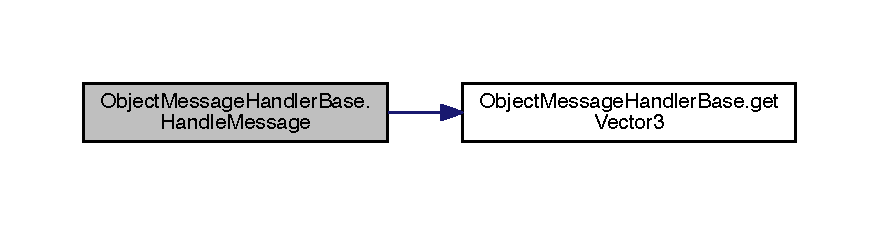
\includegraphics[width=350pt]{group___o_m_h___commands_ga86c01c29831daf58f5b0ecc3ce65ee58_cgraph}
\end{center}
\end{figure}



\chapter{Namespace Documentation}
\hypertarget{namespace_b83}{}\section{B83 Namespace Reference}
\label{namespace_b83}\index{B83@{B83}}
\subsection*{Namespaces}
\begin{DoxyCompactItemize}
\end{DoxyCompactItemize}

\hypertarget{namespace_b83_1_1_logic_expression_parser}{}\section{B83.\+Logic\+Expression\+Parser Namespace Reference}
\label{namespace_b83_1_1_logic_expression_parser}\index{B83.\+Logic\+Expression\+Parser@{B83.\+Logic\+Expression\+Parser}}
\subsection*{Classes}
\begin{DoxyCompactItemize}
\item 
class \hyperlink{class_b83_1_1_logic_expression_parser_1_1_bool_to_number}{Bool\+To\+Number}
\item 
class \hyperlink{class_b83_1_1_logic_expression_parser_1_1_combine_and}{Combine\+And}
\item 
class \hyperlink{class_b83_1_1_logic_expression_parser_1_1_combine_not}{Combine\+Not}
\item 
class \hyperlink{class_b83_1_1_logic_expression_parser_1_1_combine_or}{Combine\+Or}
\item 
class \hyperlink{class_b83_1_1_logic_expression_parser_1_1_combine_xor}{Combine\+Xor}
\item 
class \hyperlink{class_b83_1_1_logic_expression_parser_1_1_compare_equal}{Compare\+Equal}
\item 
class \hyperlink{class_b83_1_1_logic_expression_parser_1_1_compare_greater}{Compare\+Greater}
\item 
class \hyperlink{class_b83_1_1_logic_expression_parser_1_1_compare_greater_or_equal}{Compare\+Greater\+Or\+Equal}
\item 
class \hyperlink{class_b83_1_1_logic_expression_parser_1_1_compare_lower}{Compare\+Lower}
\item 
class \hyperlink{class_b83_1_1_logic_expression_parser_1_1_compare_lower_or_equal}{Compare\+Lower\+Or\+Equal}
\item 
class \hyperlink{class_b83_1_1_logic_expression_parser_1_1_compare_not_equal}{Compare\+Not\+Equal}
\item 
class \hyperlink{class_b83_1_1_logic_expression_parser_1_1_compare_statement}{Compare\+Statement}
\item 
class \hyperlink{class_b83_1_1_logic_expression_parser_1_1_constant_bool}{Constant\+Bool}
\item 
class \hyperlink{class_b83_1_1_logic_expression_parser_1_1_constant_number}{Constant\+Number}
\item 
class \hyperlink{class_b83_1_1_logic_expression_parser_1_1_constant_string}{Constant\+String}
\item 
class \hyperlink{class_b83_1_1_logic_expression_parser_1_1_custom_function}{Custom\+Function}
\item 
class \hyperlink{class_b83_1_1_logic_expression_parser_1_1_custom_string_function}{Custom\+String\+Function}
\item 
class \hyperlink{class_b83_1_1_logic_expression_parser_1_1_delegate_bool}{Delegate\+Bool}
\item 
class \hyperlink{class_b83_1_1_logic_expression_parser_1_1_delegate_number}{Delegate\+Number}
\item 
class \hyperlink{class_b83_1_1_logic_expression_parser_1_1_delegate_string}{Delegate\+String}
\item 
class \hyperlink{class_b83_1_1_logic_expression_parser_1_1_expression_context}{Expression\+Context}
\item 
class \hyperlink{class_b83_1_1_logic_expression_parser_1_1_expression_variable}{Expression\+Variable}
\item 
interface \hyperlink{interface_b83_1_1_logic_expression_parser_1_1_i_command_parser}{I\+Command\+Parser}
\item 
interface \hyperlink{interface_b83_1_1_logic_expression_parser_1_1_i_logic_result}{I\+Logic\+Result}
\item 
interface \hyperlink{interface_b83_1_1_logic_expression_parser_1_1_i_number_provider}{I\+Number\+Provider}
\item 
interface \hyperlink{interface_b83_1_1_logic_expression_parser_1_1_i_string_provider}{I\+String\+Provider}
\item 
class \hyperlink{class_b83_1_1_logic_expression_parser_1_1_logic_expression}{Logic\+Expression}
\item 
class \hyperlink{class_b83_1_1_logic_expression_parser_1_1_number_expression}{Number\+Expression}
\item 
class \hyperlink{class_b83_1_1_logic_expression_parser_1_1_number_to_bool}{Number\+To\+Bool}
\item 
class \hyperlink{class_b83_1_1_logic_expression_parser_1_1_operation_add}{Operation\+Add}
\item 
class \hyperlink{class_b83_1_1_logic_expression_parser_1_1_operation_concat}{Operation\+Concat}
\item 
class \hyperlink{class_b83_1_1_logic_expression_parser_1_1_operation_negate}{Operation\+Negate}
\item 
class \hyperlink{class_b83_1_1_logic_expression_parser_1_1_operation_power}{Operation\+Power}
\item 
class \hyperlink{class_b83_1_1_logic_expression_parser_1_1_operation_product}{Operation\+Product}
\item 
class \hyperlink{class_b83_1_1_logic_expression_parser_1_1_operation_reciprocal}{Operation\+Reciprocal}
\item 
class \hyperlink{class_b83_1_1_logic_expression_parser_1_1_parameter_list}{Parameter\+List}
\item 
class \hyperlink{class_b83_1_1_logic_expression_parser_1_1_parse_exception}{Parse\+Exception}
\item 
class \hyperlink{class_b83_1_1_logic_expression_parser_1_1_parser}{Parser}
\item 
class \hyperlink{class_b83_1_1_logic_expression_parser_1_1_parsing_context}{Parsing\+Context}
\item 
class \hyperlink{class_b83_1_1_logic_expression_parser_1_1_string_expression}{String\+Expression}
\item 
class \hyperlink{class_b83_1_1_logic_expression_parser_1_1_value_provider}{Value\+Provider}
\end{DoxyCompactItemize}

\hypertarget{namespace_little_brain}{}\section{Little\+Brain Namespace Reference}
\label{namespace_little_brain}\index{Little\+Brain@{Little\+Brain}}
\subsection*{Namespaces}
\begin{DoxyCompactItemize}
\end{DoxyCompactItemize}

\hypertarget{namespace_little_brain_1_1_g_m_addr}{}\section{Little\+Brain.\+G\+M\+Addr Namespace Reference}
\label{namespace_little_brain_1_1_g_m_addr}\index{Little\+Brain.\+G\+M\+Addr@{Little\+Brain.\+G\+M\+Addr}}
\subsection*{Classes}
\begin{DoxyCompactItemize}
\item 
class \hyperlink{class_little_brain_1_1_g_m_addr_1_1_command_sequence}{Command\+Sequence}
\item 
class \hyperlink{class_little_brain_1_1_g_m_addr_1_1_expression_parser}{Expression\+Parser}
\item 
class {\bfseries Extensions}
\item 
class \hyperlink{class_little_brain_1_1_g_m_addr_1_1_my_game_manager_addr}{My\+Game\+Manager\+Addr}
\item 
class \hyperlink{class_little_brain_1_1_g_m_addr_1_1_param_data}{Param\+Data}
\end{DoxyCompactItemize}
\subsection*{Enumerations}
\begin{DoxyCompactItemize}
\item 
enum {\bfseries Data\+Type} \{ {\bfseries Number}, 
{\bfseries Bool}, 
{\bfseries String}
 \}\hypertarget{namespace_little_brain_1_1_g_m_addr_ab822df7ff79cd3549adc2758596374f4}{}\label{namespace_little_brain_1_1_g_m_addr_ab822df7ff79cd3549adc2758596374f4}

\end{DoxyCompactItemize}

\hypertarget{namespace_unity_template_projects}{}\section{Unity\+Template\+Projects Namespace Reference}
\label{namespace_unity_template_projects}\index{Unity\+Template\+Projects@{Unity\+Template\+Projects}}
\subsection*{Classes}
\begin{DoxyCompactItemize}
\item 
class \hyperlink{class_unity_template_projects_1_1_simple_camera_controller}{Simple\+Camera\+Controller}
\end{DoxyCompactItemize}

\chapter{Class Documentation}
\hypertarget{class_back_controller}{}\section{Back\+Controller Class Reference}
\label{class_back_controller}\index{Back\+Controller@{Back\+Controller}}


Inheritance diagram for Back\+Controller\+:\nopagebreak
\begin{figure}[H]
\begin{center}
\leavevmode
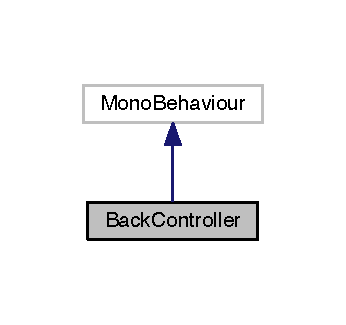
\includegraphics[width=166pt]{class_back_controller__inherit__graph}
\end{center}
\end{figure}


Collaboration diagram for Back\+Controller\+:\nopagebreak
\begin{figure}[H]
\begin{center}
\leavevmode
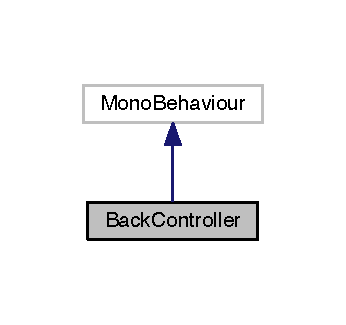
\includegraphics[width=166pt]{class_back_controller__coll__graph}
\end{center}
\end{figure}


The documentation for this class was generated from the following file\+:\begin{DoxyCompactItemize}
\item 
/\+Users/pjd37/\+Documents/\+Git\+Hub/\+Blood\+Transfusion/\+B\+T/\+Assets/\+Scripts/\+Prototyping/Back\+Controller.\+cs\end{DoxyCompactItemize}

\hypertarget{class_b83_1_1_logic_expression_parser_1_1_bool_to_number}{}\section{B83.\+Logic\+Expression\+Parser.\+Bool\+To\+Number Class Reference}
\label{class_b83_1_1_logic_expression_parser_1_1_bool_to_number}\index{B83.\+Logic\+Expression\+Parser.\+Bool\+To\+Number@{B83.\+Logic\+Expression\+Parser.\+Bool\+To\+Number}}


Inheritance diagram for B83.\+Logic\+Expression\+Parser.\+Bool\+To\+Number\+:\nopagebreak
\begin{figure}[H]
\begin{center}
\leavevmode
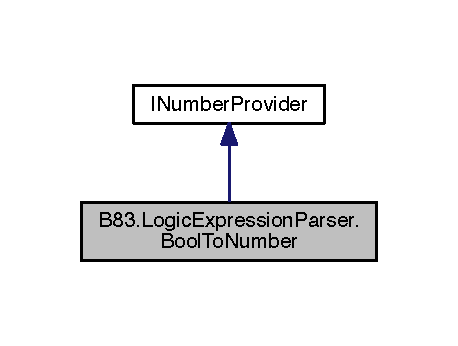
\includegraphics[width=220pt]{class_b83_1_1_logic_expression_parser_1_1_bool_to_number__inherit__graph}
\end{center}
\end{figure}


Collaboration diagram for B83.\+Logic\+Expression\+Parser.\+Bool\+To\+Number\+:\nopagebreak
\begin{figure}[H]
\begin{center}
\leavevmode
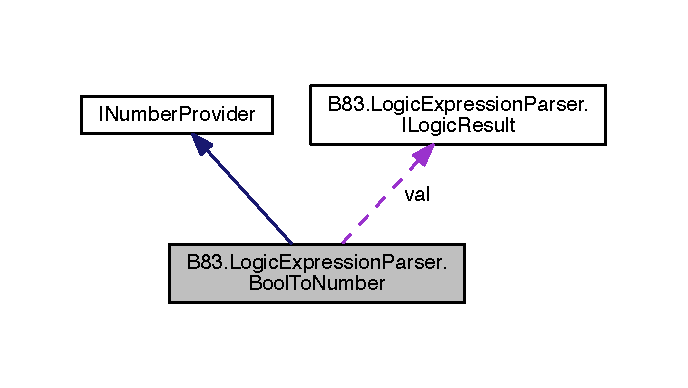
\includegraphics[width=330pt]{class_b83_1_1_logic_expression_parser_1_1_bool_to_number__coll__graph}
\end{center}
\end{figure}
\subsection*{Public Member Functions}
\begin{DoxyCompactItemize}
\item 
bool {\bfseries Is\+String} ()\hypertarget{class_b83_1_1_logic_expression_parser_1_1_bool_to_number_a30da2f89cd17cddc27b80f1c44cfcfd9}{}\label{class_b83_1_1_logic_expression_parser_1_1_bool_to_number_a30da2f89cd17cddc27b80f1c44cfcfd9}

\item 
double {\bfseries Get\+Number} ()\hypertarget{class_b83_1_1_logic_expression_parser_1_1_bool_to_number_a42ef33a0ea2919f001c6c6d8686c72e4}{}\label{class_b83_1_1_logic_expression_parser_1_1_bool_to_number_a42ef33a0ea2919f001c6c6d8686c72e4}

\end{DoxyCompactItemize}
\subsection*{Public Attributes}
\begin{DoxyCompactItemize}
\item 
\hyperlink{interface_b83_1_1_logic_expression_parser_1_1_i_logic_result}{I\+Logic\+Result} {\bfseries val}\hypertarget{class_b83_1_1_logic_expression_parser_1_1_bool_to_number_ac92de1d55cc5a359946315fc1d455c66}{}\label{class_b83_1_1_logic_expression_parser_1_1_bool_to_number_ac92de1d55cc5a359946315fc1d455c66}

\end{DoxyCompactItemize}


The documentation for this class was generated from the following file\+:\begin{DoxyCompactItemize}
\item 
/\+Users/pjd37/\+Documents/\+Git\+Hub/\+Blood\+Transfusion/\+B\+T/\+Assets/\+Scripts/Expr\+Test.\+cs\end{DoxyCompactItemize}

\hypertarget{class_monitor_updates_1_1_b_p_tween}{}\section{Monitor\+Updates.\+B\+P\+Tween Class Reference}
\label{class_monitor_updates_1_1_b_p_tween}\index{Monitor\+Updates.\+B\+P\+Tween@{Monitor\+Updates.\+B\+P\+Tween}}


Inheritance diagram for Monitor\+Updates.\+B\+P\+Tween\+:\nopagebreak
\begin{figure}[H]
\begin{center}
\leavevmode
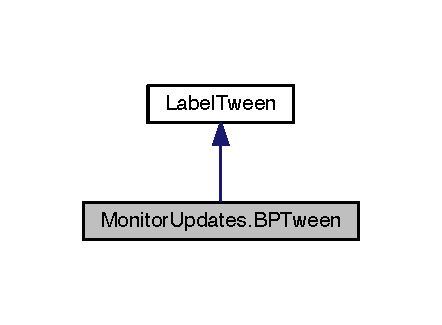
\includegraphics[width=212pt]{class_monitor_updates_1_1_b_p_tween__inherit__graph}
\end{center}
\end{figure}


Collaboration diagram for Monitor\+Updates.\+B\+P\+Tween\+:\nopagebreak
\begin{figure}[H]
\begin{center}
\leavevmode
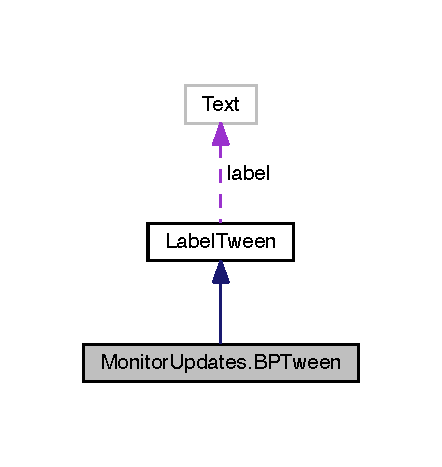
\includegraphics[width=212pt]{class_monitor_updates_1_1_b_p_tween__coll__graph}
\end{center}
\end{figure}
\subsection*{Public Member Functions}
\begin{DoxyCompactItemize}
\item 
{\bfseries B\+P\+Tween} (float l, Text lbl, float t, string format, float start\+Val, float bot\+Start, float bot\+Tar)\hypertarget{class_monitor_updates_1_1_b_p_tween_af79344953acaad6ab9a83cc7570ca66c}{}\label{class_monitor_updates_1_1_b_p_tween_af79344953acaad6ab9a83cc7570ca66c}

\end{DoxyCompactItemize}
\subsection*{Public Attributes}
\begin{DoxyCompactItemize}
\item 
float {\bfseries bot\+Start}\hypertarget{class_monitor_updates_1_1_b_p_tween_a21f346b5d00e4421c0f5f0f54dd64e51}{}\label{class_monitor_updates_1_1_b_p_tween_a21f346b5d00e4421c0f5f0f54dd64e51}

\item 
float {\bfseries bot\+Target}\hypertarget{class_monitor_updates_1_1_b_p_tween_a5637121fb9ae7a8b18c990bedf1cbf13}{}\label{class_monitor_updates_1_1_b_p_tween_a5637121fb9ae7a8b18c990bedf1cbf13}

\end{DoxyCompactItemize}


The documentation for this class was generated from the following file\+:\begin{DoxyCompactItemize}
\item 
/\+Users/pjd37/\+Documents/\+Git\+Hub/\+Blood\+Transfusion/\+B\+T/\+Assets/\+Scripts/\+Heart\+Monitor/Monitor\+Updates.\+cs\end{DoxyCompactItemize}

\hypertarget{class_button}{}\section{Button Class Reference}
\label{class_button}\index{Button@{Button}}


Inheritance diagram for Button\+:\nopagebreak
\begin{figure}[H]
\begin{center}
\leavevmode
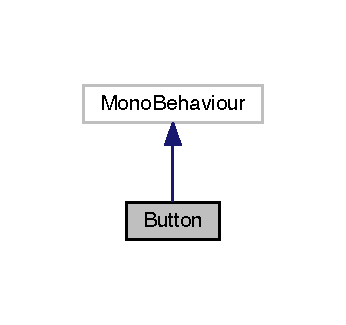
\includegraphics[width=166pt]{class_button__inherit__graph}
\end{center}
\end{figure}


Collaboration diagram for Button\+:\nopagebreak
\begin{figure}[H]
\begin{center}
\leavevmode
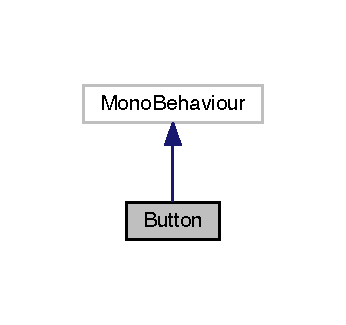
\includegraphics[width=166pt]{class_button__coll__graph}
\end{center}
\end{figure}
\subsection*{Public Member Functions}
\begin{DoxyCompactItemize}
\item 
virtual bool {\bfseries Handle\+Message} (string msg, string param=null)\hypertarget{class_button_aac84d9ad4a1126ce1ccdfc719d1b9356}{}\label{class_button_aac84d9ad4a1126ce1ccdfc719d1b9356}

\item 
void {\bfseries Pressed} ()\hypertarget{class_button_a32acc0b75cda56a10936fb4590d52826}{}\label{class_button_a32acc0b75cda56a10936fb4590d52826}

\end{DoxyCompactItemize}
\subsection*{Public Attributes}
\begin{DoxyCompactItemize}
\item 
bool {\bfseries pressed} = false\hypertarget{class_button_a7ac9f95924e2004cf80666ae1952f39e}{}\label{class_button_a7ac9f95924e2004cf80666ae1952f39e}

\end{DoxyCompactItemize}


The documentation for this class was generated from the following file\+:\begin{DoxyCompactItemize}
\item 
/\+Users/pjd37/\+Documents/\+Git\+Hub/\+Blood\+Transfusion/\+B\+T/\+Assets/\+Scripts/Button.\+cs\end{DoxyCompactItemize}

\hypertarget{class_camera_raycast_test}{}\section{Camera\+Raycast\+Test Class Reference}
\label{class_camera_raycast_test}\index{Camera\+Raycast\+Test@{Camera\+Raycast\+Test}}


Inheritance diagram for Camera\+Raycast\+Test\+:\nopagebreak
\begin{figure}[H]
\begin{center}
\leavevmode
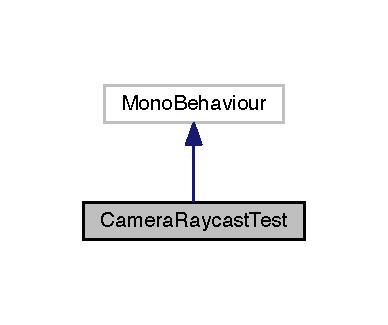
\includegraphics[width=186pt]{class_camera_raycast_test__inherit__graph}
\end{center}
\end{figure}


Collaboration diagram for Camera\+Raycast\+Test\+:\nopagebreak
\begin{figure}[H]
\begin{center}
\leavevmode
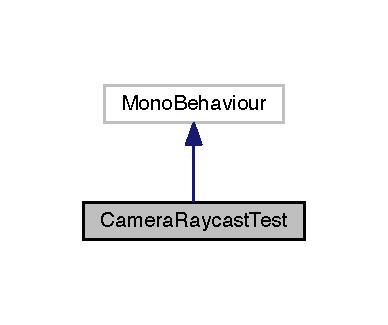
\includegraphics[width=186pt]{class_camera_raycast_test__coll__graph}
\end{center}
\end{figure}


The documentation for this class was generated from the following file\+:\begin{DoxyCompactItemize}
\item 
/\+Users/pjd37/\+Documents/\+Git\+Hub/\+Blood\+Transfusion/\+B\+T/\+Assets/\+Scripts/\+Camera/Camera\+Raycast\+Test.\+cs\end{DoxyCompactItemize}

\hypertarget{class_camera_target_params}{}\section{Camera\+Target\+Params Class Reference}
\label{class_camera_target_params}\index{Camera\+Target\+Params@{Camera\+Target\+Params}}


\hyperlink{class_camera_target_params}{Camera\+Target\+Params}  




Inheritance diagram for Camera\+Target\+Params\+:\nopagebreak
\begin{figure}[H]
\begin{center}
\leavevmode
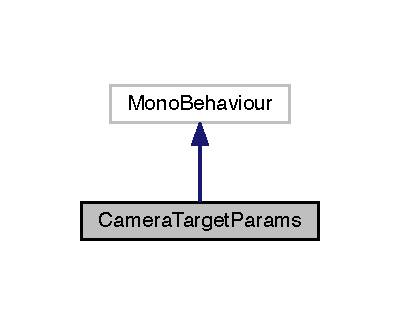
\includegraphics[width=192pt]{class_camera_target_params__inherit__graph}
\end{center}
\end{figure}


Collaboration diagram for Camera\+Target\+Params\+:\nopagebreak
\begin{figure}[H]
\begin{center}
\leavevmode
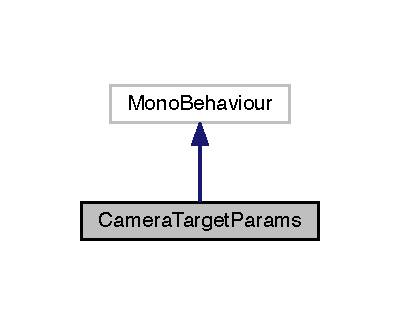
\includegraphics[width=192pt]{class_camera_target_params__coll__graph}
\end{center}
\end{figure}
\subsection*{Public Attributes}
\begin{DoxyCompactItemize}
\item 
Transform {\bfseries close}\hypertarget{class_camera_target_params_afa7fabcf3f06c61d279e3476aeacbed7}{}\label{class_camera_target_params_afa7fabcf3f06c61d279e3476aeacbed7}

\item 
Transform {\bfseries medium}\hypertarget{class_camera_target_params_ad4a03429eb8225098a060c12b90c98bf}{}\label{class_camera_target_params_ad4a03429eb8225098a060c12b90c98bf}

\item 
Transform {\bfseries far}\hypertarget{class_camera_target_params_aa26025a0caf9f8fa5387924c44c675ff}{}\label{class_camera_target_params_aa26025a0caf9f8fa5387924c44c675ff}

\item 
Transform {\bfseries look\+At}\hypertarget{class_camera_target_params_ab395ee0b4573564121ba9b6f39de7e4b}{}\label{class_camera_target_params_ab395ee0b4573564121ba9b6f39de7e4b}

\end{DoxyCompactItemize}


\subsection{Detailed Description}
\hyperlink{class_camera_target_params}{Camera\+Target\+Params} 


\begin{DoxyParams}{Parameters}
{\em close} & Camera position for close up shot of this object.\\
\hline
{\em medium} & Camera position for medium shot of this object.\\
\hline
{\em far} & Camera position for far shot of this object.\\
\hline
{\em look\+At} & Target position for camera to look at this object.\\
\hline
\end{DoxyParams}


The documentation for this class was generated from the following file\+:\begin{DoxyCompactItemize}
\item 
/\+Users/pjd37/\+Documents/\+Git\+Hub/\+Blood\+Transfusion/\+B\+T/\+Assets/\+Scripts/\+Camera/Camera\+Target\+Params.\+cs\end{DoxyCompactItemize}

\hypertarget{class_b83_1_1_logic_expression_parser_1_1_combine_and}{}\section{B83.\+Logic\+Expression\+Parser.\+Combine\+And Class Reference}
\label{class_b83_1_1_logic_expression_parser_1_1_combine_and}\index{B83.\+Logic\+Expression\+Parser.\+Combine\+And@{B83.\+Logic\+Expression\+Parser.\+Combine\+And}}


Inheritance diagram for B83.\+Logic\+Expression\+Parser.\+Combine\+And\+:\nopagebreak
\begin{figure}[H]
\begin{center}
\leavevmode
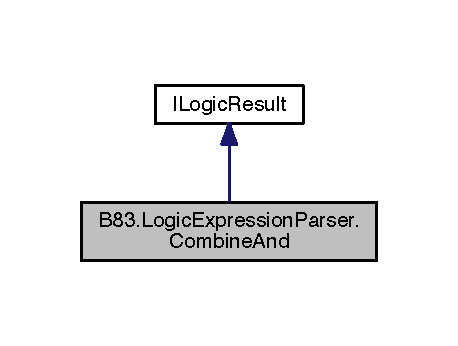
\includegraphics[width=220pt]{class_b83_1_1_logic_expression_parser_1_1_combine_and__inherit__graph}
\end{center}
\end{figure}


Collaboration diagram for B83.\+Logic\+Expression\+Parser.\+Combine\+And\+:\nopagebreak
\begin{figure}[H]
\begin{center}
\leavevmode
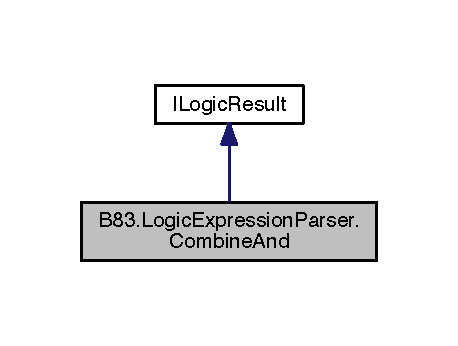
\includegraphics[width=220pt]{class_b83_1_1_logic_expression_parser_1_1_combine_and__coll__graph}
\end{center}
\end{figure}
\subsection*{Public Member Functions}
\begin{DoxyCompactItemize}
\item 
bool {\bfseries Get\+Result} ()\hypertarget{class_b83_1_1_logic_expression_parser_1_1_combine_and_a23fd421aee4a42e3c478b5326325088a}{}\label{class_b83_1_1_logic_expression_parser_1_1_combine_and_a23fd421aee4a42e3c478b5326325088a}

\end{DoxyCompactItemize}
\subsection*{Public Attributes}
\begin{DoxyCompactItemize}
\item 
List$<$ \hyperlink{interface_b83_1_1_logic_expression_parser_1_1_i_logic_result}{I\+Logic\+Result} $>$ {\bfseries inputs} = new List$<$\hyperlink{interface_b83_1_1_logic_expression_parser_1_1_i_logic_result}{I\+Logic\+Result}$>$()\hypertarget{class_b83_1_1_logic_expression_parser_1_1_combine_and_a216fe9a1a06220498f6dcc010f6b5d3e}{}\label{class_b83_1_1_logic_expression_parser_1_1_combine_and_a216fe9a1a06220498f6dcc010f6b5d3e}

\end{DoxyCompactItemize}


The documentation for this class was generated from the following file\+:\begin{DoxyCompactItemize}
\item 
/\+Users/pjd37/\+Documents/\+Git\+Hub/\+Blood\+Transfusion/\+B\+T/\+Assets/\+Scripts/Expr\+Test.\+cs\end{DoxyCompactItemize}

\hypertarget{class_b83_1_1_logic_expression_parser_1_1_combine_not}{}\section{B83.\+Logic\+Expression\+Parser.\+Combine\+Not Class Reference}
\label{class_b83_1_1_logic_expression_parser_1_1_combine_not}\index{B83.\+Logic\+Expression\+Parser.\+Combine\+Not@{B83.\+Logic\+Expression\+Parser.\+Combine\+Not}}


Inheritance diagram for B83.\+Logic\+Expression\+Parser.\+Combine\+Not\+:\nopagebreak
\begin{figure}[H]
\begin{center}
\leavevmode
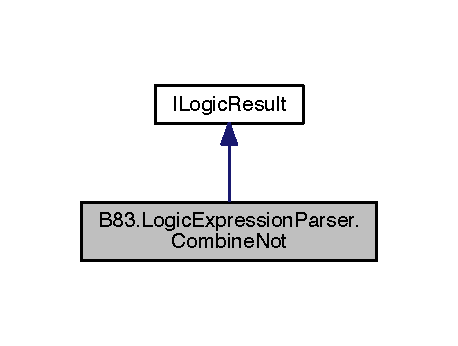
\includegraphics[width=220pt]{class_b83_1_1_logic_expression_parser_1_1_combine_not__inherit__graph}
\end{center}
\end{figure}


Collaboration diagram for B83.\+Logic\+Expression\+Parser.\+Combine\+Not\+:\nopagebreak
\begin{figure}[H]
\begin{center}
\leavevmode
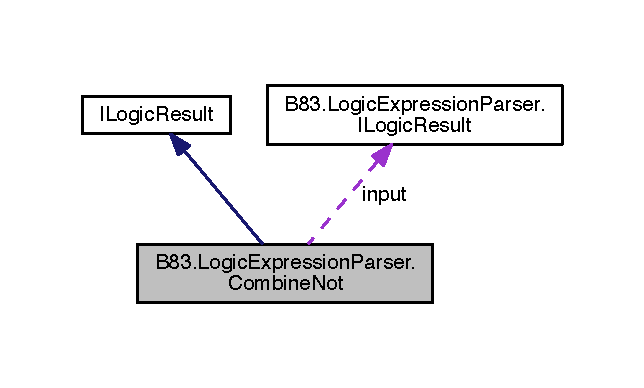
\includegraphics[width=309pt]{class_b83_1_1_logic_expression_parser_1_1_combine_not__coll__graph}
\end{center}
\end{figure}
\subsection*{Public Member Functions}
\begin{DoxyCompactItemize}
\item 
bool {\bfseries Get\+Result} ()\hypertarget{class_b83_1_1_logic_expression_parser_1_1_combine_not_a6fd9cc22b208fa90678d9892c2382185}{}\label{class_b83_1_1_logic_expression_parser_1_1_combine_not_a6fd9cc22b208fa90678d9892c2382185}

\end{DoxyCompactItemize}
\subsection*{Public Attributes}
\begin{DoxyCompactItemize}
\item 
\hyperlink{interface_b83_1_1_logic_expression_parser_1_1_i_logic_result}{I\+Logic\+Result} {\bfseries input}\hypertarget{class_b83_1_1_logic_expression_parser_1_1_combine_not_ad9d454db466343baf3054a70880f937e}{}\label{class_b83_1_1_logic_expression_parser_1_1_combine_not_ad9d454db466343baf3054a70880f937e}

\end{DoxyCompactItemize}


The documentation for this class was generated from the following file\+:\begin{DoxyCompactItemize}
\item 
/\+Users/pjd37/\+Documents/\+Git\+Hub/\+Blood\+Transfusion/\+B\+T/\+Assets/\+Scripts/Expr\+Test.\+cs\end{DoxyCompactItemize}

\hypertarget{class_b83_1_1_logic_expression_parser_1_1_combine_or}{}\section{B83.\+Logic\+Expression\+Parser.\+Combine\+Or Class Reference}
\label{class_b83_1_1_logic_expression_parser_1_1_combine_or}\index{B83.\+Logic\+Expression\+Parser.\+Combine\+Or@{B83.\+Logic\+Expression\+Parser.\+Combine\+Or}}


Inheritance diagram for B83.\+Logic\+Expression\+Parser.\+Combine\+Or\+:\nopagebreak
\begin{figure}[H]
\begin{center}
\leavevmode
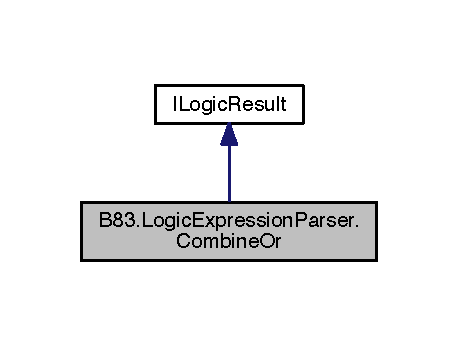
\includegraphics[width=220pt]{class_b83_1_1_logic_expression_parser_1_1_combine_or__inherit__graph}
\end{center}
\end{figure}


Collaboration diagram for B83.\+Logic\+Expression\+Parser.\+Combine\+Or\+:\nopagebreak
\begin{figure}[H]
\begin{center}
\leavevmode
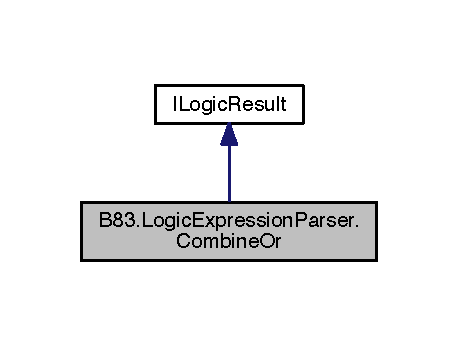
\includegraphics[width=220pt]{class_b83_1_1_logic_expression_parser_1_1_combine_or__coll__graph}
\end{center}
\end{figure}
\subsection*{Public Member Functions}
\begin{DoxyCompactItemize}
\item 
bool {\bfseries Get\+Result} ()\hypertarget{class_b83_1_1_logic_expression_parser_1_1_combine_or_a1c908a08374a66cbcfced23d29d494de}{}\label{class_b83_1_1_logic_expression_parser_1_1_combine_or_a1c908a08374a66cbcfced23d29d494de}

\end{DoxyCompactItemize}
\subsection*{Public Attributes}
\begin{DoxyCompactItemize}
\item 
List$<$ \hyperlink{interface_b83_1_1_logic_expression_parser_1_1_i_logic_result}{I\+Logic\+Result} $>$ {\bfseries inputs} = new List$<$\hyperlink{interface_b83_1_1_logic_expression_parser_1_1_i_logic_result}{I\+Logic\+Result}$>$()\hypertarget{class_b83_1_1_logic_expression_parser_1_1_combine_or_ae54fe96dcdb87536a29aab8df14f8ffc}{}\label{class_b83_1_1_logic_expression_parser_1_1_combine_or_ae54fe96dcdb87536a29aab8df14f8ffc}

\end{DoxyCompactItemize}


The documentation for this class was generated from the following file\+:\begin{DoxyCompactItemize}
\item 
/\+Users/pjd37/\+Documents/\+Git\+Hub/\+Blood\+Transfusion/\+B\+T/\+Assets/\+Scripts/Expr\+Test.\+cs\end{DoxyCompactItemize}

\hypertarget{class_b83_1_1_logic_expression_parser_1_1_combine_xor}{}\section{B83.\+Logic\+Expression\+Parser.\+Combine\+Xor Class Reference}
\label{class_b83_1_1_logic_expression_parser_1_1_combine_xor}\index{B83.\+Logic\+Expression\+Parser.\+Combine\+Xor@{B83.\+Logic\+Expression\+Parser.\+Combine\+Xor}}


Inheritance diagram for B83.\+Logic\+Expression\+Parser.\+Combine\+Xor\+:\nopagebreak
\begin{figure}[H]
\begin{center}
\leavevmode
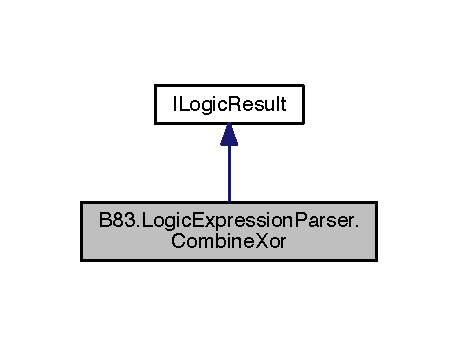
\includegraphics[width=220pt]{class_b83_1_1_logic_expression_parser_1_1_combine_xor__inherit__graph}
\end{center}
\end{figure}


Collaboration diagram for B83.\+Logic\+Expression\+Parser.\+Combine\+Xor\+:\nopagebreak
\begin{figure}[H]
\begin{center}
\leavevmode
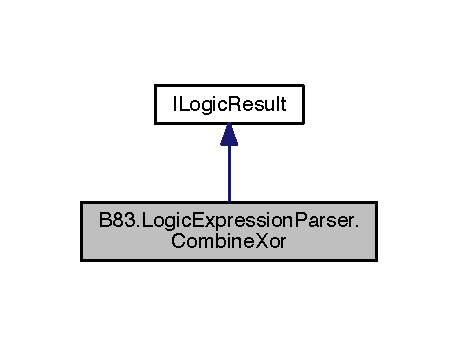
\includegraphics[width=220pt]{class_b83_1_1_logic_expression_parser_1_1_combine_xor__coll__graph}
\end{center}
\end{figure}
\subsection*{Public Member Functions}
\begin{DoxyCompactItemize}
\item 
bool {\bfseries Get\+Result} ()\hypertarget{class_b83_1_1_logic_expression_parser_1_1_combine_xor_a1b621ac78c2edcecf005dfe371eb1651}{}\label{class_b83_1_1_logic_expression_parser_1_1_combine_xor_a1b621ac78c2edcecf005dfe371eb1651}

\end{DoxyCompactItemize}
\subsection*{Public Attributes}
\begin{DoxyCompactItemize}
\item 
List$<$ \hyperlink{interface_b83_1_1_logic_expression_parser_1_1_i_logic_result}{I\+Logic\+Result} $>$ {\bfseries inputs} = new List$<$\hyperlink{interface_b83_1_1_logic_expression_parser_1_1_i_logic_result}{I\+Logic\+Result}$>$()\hypertarget{class_b83_1_1_logic_expression_parser_1_1_combine_xor_ac82995b6a5337ebfd0aa3cc9c633fb2c}{}\label{class_b83_1_1_logic_expression_parser_1_1_combine_xor_ac82995b6a5337ebfd0aa3cc9c633fb2c}

\end{DoxyCompactItemize}


The documentation for this class was generated from the following file\+:\begin{DoxyCompactItemize}
\item 
/\+Users/pjd37/\+Documents/\+Git\+Hub/\+Blood\+Transfusion/\+B\+T/\+Assets/\+Scripts/Expr\+Test.\+cs\end{DoxyCompactItemize}

\hypertarget{class_command_sequence}{}\section{Command\+Sequence Class Reference}
\label{class_command_sequence}\index{Command\+Sequence@{Command\+Sequence}}
\subsection*{Public Types}
\begin{DoxyCompactItemize}
\item 
enum {\bfseries I\+F\+State} \{ {\bfseries False}, 
{\bfseries Condition}, 
{\bfseries Then}, 
{\bfseries Else}
 \}\hypertarget{class_command_sequence_a6e011a1e2a227e35f01d2cfca4317f01}{}\label{class_command_sequence_a6e011a1e2a227e35f01d2cfca4317f01}

\item 
enum {\bfseries W\+A\+I\+T\+State} \{ {\bfseries False}, 
{\bfseries Condition}, 
{\bfseries Condition\+Any}, 
{\bfseries Condition\+All}
 \}\hypertarget{class_command_sequence_a6963cfe8aa56995c00e22876e7d577f2}{}\label{class_command_sequence_a6963cfe8aa56995c00e22876e7d577f2}

\item 
enum {\bfseries C\+H\+O\+I\+C\+E\+State} \{ {\bfseries False}, 
{\bfseries Choice}, 
{\bfseries Not\+Choice}
 \}\hypertarget{class_command_sequence_aac8973304c0f788b69b6ebb1c6bd16a8}{}\label{class_command_sequence_aac8973304c0f788b69b6ebb1c6bd16a8}

\end{DoxyCompactItemize}
\subsection*{Public Attributes}
\begin{DoxyCompactItemize}
\item 
string {\bfseries file\+Name}\hypertarget{class_command_sequence_a0b9b187c090f1b088518adb802b343d8}{}\label{class_command_sequence_a0b9b187c090f1b088518adb802b343d8}

\item 
int {\bfseries command\+Num} = 0\hypertarget{class_command_sequence_afe13c8bfa11220d47874dd3da1d92926}{}\label{class_command_sequence_afe13c8bfa11220d47874dd3da1d92926}

\item 
I\+F\+State {\bfseries I\+Fstate} = I\+F\+State.\+False\hypertarget{class_command_sequence_ac1302445b2951efaa118750ebcece9af}{}\label{class_command_sequence_ac1302445b2951efaa118750ebcece9af}

\item 
W\+A\+I\+T\+State {\bfseries W\+A\+I\+Tstate} = W\+A\+I\+T\+State.\+False\hypertarget{class_command_sequence_a948d080c59b810522789322e52f4fd8c}{}\label{class_command_sequence_a948d080c59b810522789322e52f4fd8c}

\item 
C\+H\+O\+I\+C\+E\+State {\bfseries C\+H\+O\+I\+C\+Estate} = C\+H\+O\+I\+C\+E\+State.\+False\hypertarget{class_command_sequence_a9c2cd280ee8ffc07fee4b5e1c7d710f6}{}\label{class_command_sequence_a9c2cd280ee8ffc07fee4b5e1c7d710f6}

\item 
bool {\bfseries I\+Fresult} = true\hypertarget{class_command_sequence_a3ce6cea704cdb07f8fb461551ba6aa38}{}\label{class_command_sequence_a3ce6cea704cdb07f8fb461551ba6aa38}

\item 
string {\bfseries command\+Line}\hypertarget{class_command_sequence_a46bb9ae9f3ba69d7232aad2874963fcb}{}\label{class_command_sequence_a46bb9ae9f3ba69d7232aad2874963fcb}

\item 
int {\bfseries nesting\+Level}\hypertarget{class_command_sequence_af5b70bab8b5855819bfe7c7ce62db106}{}\label{class_command_sequence_af5b70bab8b5855819bfe7c7ce62db106}

\end{DoxyCompactItemize}


The documentation for this class was generated from the following file\+:\begin{DoxyCompactItemize}
\item 
/\+Users/pjd37/\+Documents/\+Git\+Hub/\+Blood\+Transfusion/\+B\+T/\+Assets/\+Scripts/My\+Game\+Manager.\+cs\end{DoxyCompactItemize}

\hypertarget{class_little_brain_1_1_g_m_addr_1_1_command_sequence}{}\section{Little\+Brain.\+G\+M\+Addr.\+Command\+Sequence Class Reference}
\label{class_little_brain_1_1_g_m_addr_1_1_command_sequence}\index{Little\+Brain.\+G\+M\+Addr.\+Command\+Sequence@{Little\+Brain.\+G\+M\+Addr.\+Command\+Sequence}}
\subsection*{Public Types}
\begin{DoxyCompactItemize}
\item 
enum {\bfseries I\+F\+State} \{ {\bfseries False}, 
{\bfseries Condition}, 
{\bfseries Then}, 
{\bfseries Else}
 \}\hypertarget{class_little_brain_1_1_g_m_addr_1_1_command_sequence_a991781cddd2dfdde3a5d60a940c0afcc}{}\label{class_little_brain_1_1_g_m_addr_1_1_command_sequence_a991781cddd2dfdde3a5d60a940c0afcc}

\item 
enum {\bfseries W\+A\+I\+T\+State} \{ {\bfseries False}, 
{\bfseries Condition}, 
{\bfseries Condition\+Any}, 
{\bfseries Condition\+All}
 \}\hypertarget{class_little_brain_1_1_g_m_addr_1_1_command_sequence_abe54e393f577b11d4ba5762c2cb7be1e}{}\label{class_little_brain_1_1_g_m_addr_1_1_command_sequence_abe54e393f577b11d4ba5762c2cb7be1e}

\item 
enum {\bfseries C\+H\+O\+I\+C\+E\+State} \{ {\bfseries False}, 
{\bfseries Choice}, 
{\bfseries Not\+Choice}
 \}\hypertarget{class_little_brain_1_1_g_m_addr_1_1_command_sequence_a7ec982a74ff2cbbf1e5b46a609553f1d}{}\label{class_little_brain_1_1_g_m_addr_1_1_command_sequence_a7ec982a74ff2cbbf1e5b46a609553f1d}

\end{DoxyCompactItemize}
\subsection*{Public Attributes}
\begin{DoxyCompactItemize}
\item 
int {\bfseries command\+Num} =0\hypertarget{class_little_brain_1_1_g_m_addr_1_1_command_sequence_a35c4bb7b05612de00d5c6e01a094f626}{}\label{class_little_brain_1_1_g_m_addr_1_1_command_sequence_a35c4bb7b05612de00d5c6e01a094f626}

\item 
I\+F\+State {\bfseries I\+Fstate} = I\+F\+State.\+False\hypertarget{class_little_brain_1_1_g_m_addr_1_1_command_sequence_a7af7b699d0171e6b40d28d7c051abd03}{}\label{class_little_brain_1_1_g_m_addr_1_1_command_sequence_a7af7b699d0171e6b40d28d7c051abd03}

\item 
W\+A\+I\+T\+State {\bfseries W\+A\+I\+Tstate} = W\+A\+I\+T\+State.\+False\hypertarget{class_little_brain_1_1_g_m_addr_1_1_command_sequence_aecda99c081f98d330c3f541a1d43c730}{}\label{class_little_brain_1_1_g_m_addr_1_1_command_sequence_aecda99c081f98d330c3f541a1d43c730}

\item 
C\+H\+O\+I\+C\+E\+State {\bfseries C\+H\+O\+I\+C\+Estate} = C\+H\+O\+I\+C\+E\+State.\+False\hypertarget{class_little_brain_1_1_g_m_addr_1_1_command_sequence_a46ccb992a5daf807840f8fb560d0f7cb}{}\label{class_little_brain_1_1_g_m_addr_1_1_command_sequence_a46ccb992a5daf807840f8fb560d0f7cb}

\item 
bool {\bfseries I\+Fresult} = true\hypertarget{class_little_brain_1_1_g_m_addr_1_1_command_sequence_a0f6747e461530b98269eba04d184ba87}{}\label{class_little_brain_1_1_g_m_addr_1_1_command_sequence_a0f6747e461530b98269eba04d184ba87}

\item 
string {\bfseries command\+Line}\hypertarget{class_little_brain_1_1_g_m_addr_1_1_command_sequence_ae653dd749edcf7dcf8f47a784f084649}{}\label{class_little_brain_1_1_g_m_addr_1_1_command_sequence_ae653dd749edcf7dcf8f47a784f084649}

\item 
int {\bfseries nesting\+Level}\hypertarget{class_little_brain_1_1_g_m_addr_1_1_command_sequence_a0450cdf9f07f92eb35c47d50e04d8351}{}\label{class_little_brain_1_1_g_m_addr_1_1_command_sequence_a0450cdf9f07f92eb35c47d50e04d8351}

\end{DoxyCompactItemize}


The documentation for this class was generated from the following file\+:\begin{DoxyCompactItemize}
\item 
/\+Users/pjd37/\+Documents/\+Git\+Hub/\+Blood\+Transfusion/\+B\+T/\+Assets/\+Scripts/My\+Game\+Manager\+Addr.\+cs\end{DoxyCompactItemize}

\hypertarget{class_b83_1_1_logic_expression_parser_1_1_compare_equal}{}\section{B83.\+Logic\+Expression\+Parser.\+Compare\+Equal Class Reference}
\label{class_b83_1_1_logic_expression_parser_1_1_compare_equal}\index{B83.\+Logic\+Expression\+Parser.\+Compare\+Equal@{B83.\+Logic\+Expression\+Parser.\+Compare\+Equal}}


Inheritance diagram for B83.\+Logic\+Expression\+Parser.\+Compare\+Equal\+:\nopagebreak
\begin{figure}[H]
\begin{center}
\leavevmode
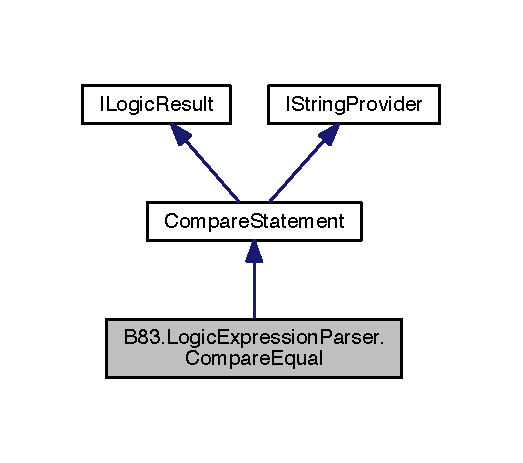
\includegraphics[width=251pt]{class_b83_1_1_logic_expression_parser_1_1_compare_equal__inherit__graph}
\end{center}
\end{figure}


Collaboration diagram for B83.\+Logic\+Expression\+Parser.\+Compare\+Equal\+:\nopagebreak
\begin{figure}[H]
\begin{center}
\leavevmode
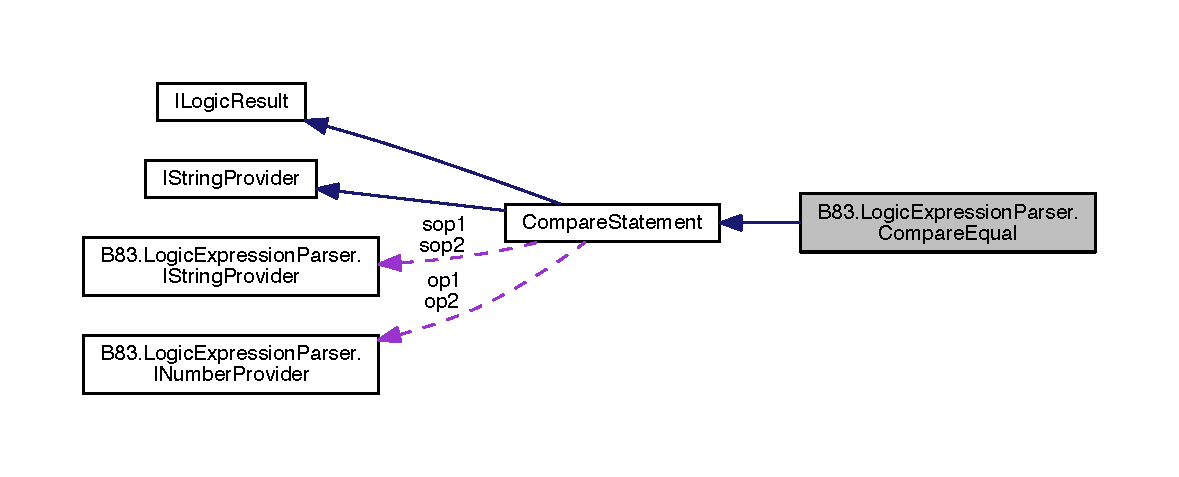
\includegraphics[width=350pt]{class_b83_1_1_logic_expression_parser_1_1_compare_equal__coll__graph}
\end{center}
\end{figure}
\subsection*{Protected Member Functions}
\begin{DoxyCompactItemize}
\item 
override bool {\bfseries Compare} (double a\+Op1, double a\+Op2)\hypertarget{class_b83_1_1_logic_expression_parser_1_1_compare_equal_a394f4479bf2581d234d639b5fa09ce9e}{}\label{class_b83_1_1_logic_expression_parser_1_1_compare_equal_a394f4479bf2581d234d639b5fa09ce9e}

\item 
override bool {\bfseries Compare} (string a\+Op1, string a\+Op2)\hypertarget{class_b83_1_1_logic_expression_parser_1_1_compare_equal_abfcbdac87bf9abbc0e99acac8eb7cfb4}{}\label{class_b83_1_1_logic_expression_parser_1_1_compare_equal_abfcbdac87bf9abbc0e99acac8eb7cfb4}

\end{DoxyCompactItemize}
\subsection*{Additional Inherited Members}


The documentation for this class was generated from the following file\+:\begin{DoxyCompactItemize}
\item 
/\+Users/pjd37/\+Documents/\+Git\+Hub/\+Blood\+Transfusion/\+B\+T/\+Assets/\+Scripts/Expr\+Test.\+cs\end{DoxyCompactItemize}

\hypertarget{class_b83_1_1_logic_expression_parser_1_1_compare_greater}{}\section{B83.\+Logic\+Expression\+Parser.\+Compare\+Greater Class Reference}
\label{class_b83_1_1_logic_expression_parser_1_1_compare_greater}\index{B83.\+Logic\+Expression\+Parser.\+Compare\+Greater@{B83.\+Logic\+Expression\+Parser.\+Compare\+Greater}}


Inheritance diagram for B83.\+Logic\+Expression\+Parser.\+Compare\+Greater\+:\nopagebreak
\begin{figure}[H]
\begin{center}
\leavevmode
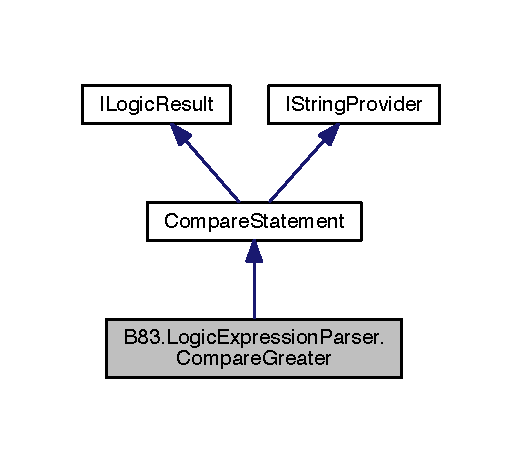
\includegraphics[width=251pt]{class_b83_1_1_logic_expression_parser_1_1_compare_greater__inherit__graph}
\end{center}
\end{figure}


Collaboration diagram for B83.\+Logic\+Expression\+Parser.\+Compare\+Greater\+:\nopagebreak
\begin{figure}[H]
\begin{center}
\leavevmode
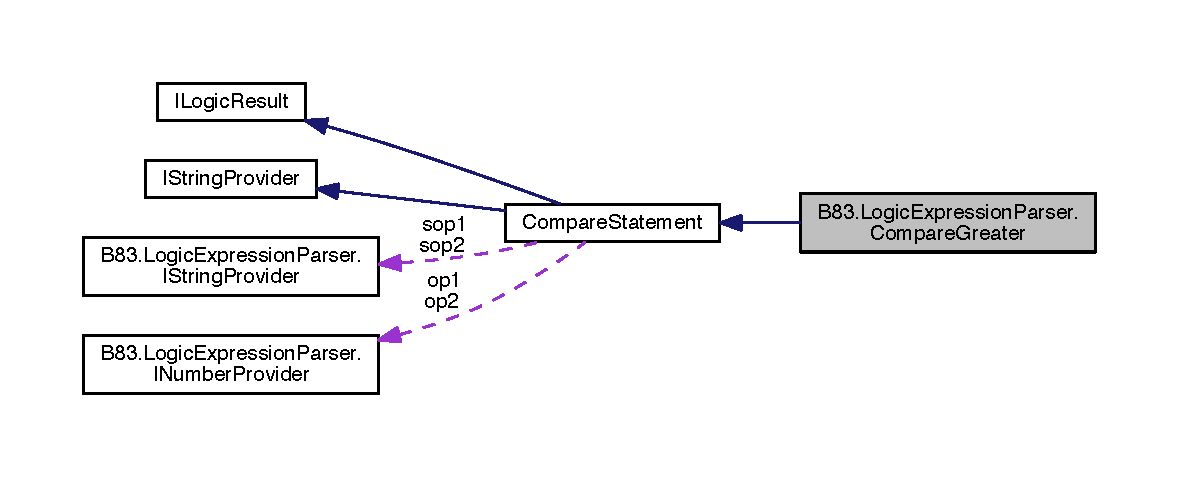
\includegraphics[width=350pt]{class_b83_1_1_logic_expression_parser_1_1_compare_greater__coll__graph}
\end{center}
\end{figure}
\subsection*{Protected Member Functions}
\begin{DoxyCompactItemize}
\item 
override bool {\bfseries Compare} (double a\+Op1, double a\+Op2)\hypertarget{class_b83_1_1_logic_expression_parser_1_1_compare_greater_a267e48f0f846f5bcaec9a89ee2284376}{}\label{class_b83_1_1_logic_expression_parser_1_1_compare_greater_a267e48f0f846f5bcaec9a89ee2284376}

\item 
override bool {\bfseries Compare} (string a\+Op1, string a\+Op2)\hypertarget{class_b83_1_1_logic_expression_parser_1_1_compare_greater_a9faf922935864bfd87b812a025a1778e}{}\label{class_b83_1_1_logic_expression_parser_1_1_compare_greater_a9faf922935864bfd87b812a025a1778e}

\end{DoxyCompactItemize}
\subsection*{Additional Inherited Members}


The documentation for this class was generated from the following file\+:\begin{DoxyCompactItemize}
\item 
/\+Users/pjd37/\+Documents/\+Git\+Hub/\+Blood\+Transfusion/\+B\+T/\+Assets/\+Scripts/Expr\+Test.\+cs\end{DoxyCompactItemize}

\hypertarget{class_b83_1_1_logic_expression_parser_1_1_compare_greater_or_equal}{}\section{B83.\+Logic\+Expression\+Parser.\+Compare\+Greater\+Or\+Equal Class Reference}
\label{class_b83_1_1_logic_expression_parser_1_1_compare_greater_or_equal}\index{B83.\+Logic\+Expression\+Parser.\+Compare\+Greater\+Or\+Equal@{B83.\+Logic\+Expression\+Parser.\+Compare\+Greater\+Or\+Equal}}


Inheritance diagram for B83.\+Logic\+Expression\+Parser.\+Compare\+Greater\+Or\+Equal\+:\nopagebreak
\begin{figure}[H]
\begin{center}
\leavevmode
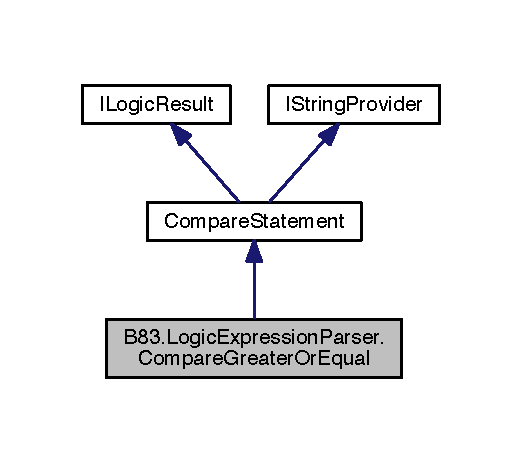
\includegraphics[width=251pt]{class_b83_1_1_logic_expression_parser_1_1_compare_greater_or_equal__inherit__graph}
\end{center}
\end{figure}


Collaboration diagram for B83.\+Logic\+Expression\+Parser.\+Compare\+Greater\+Or\+Equal\+:\nopagebreak
\begin{figure}[H]
\begin{center}
\leavevmode
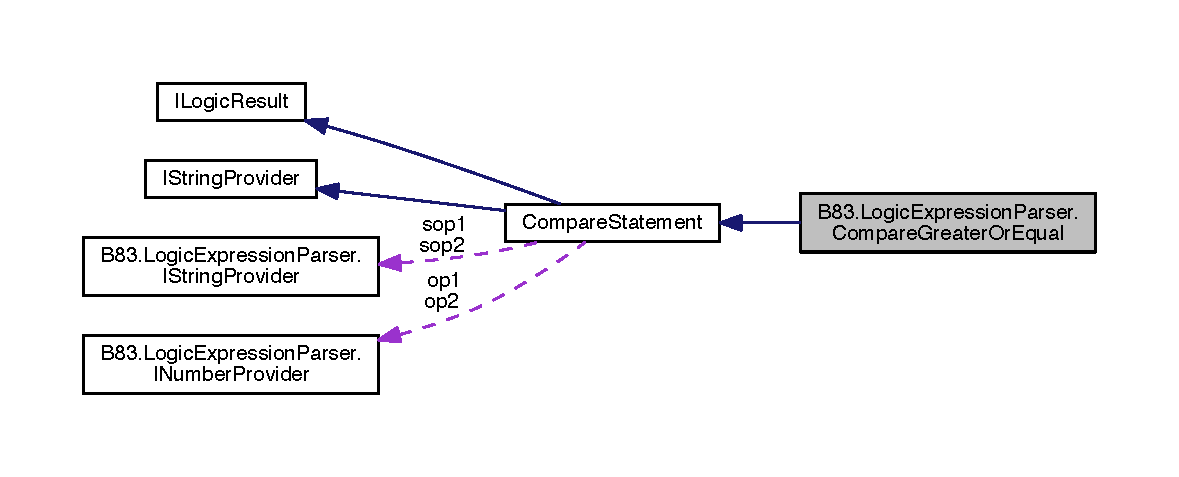
\includegraphics[width=350pt]{class_b83_1_1_logic_expression_parser_1_1_compare_greater_or_equal__coll__graph}
\end{center}
\end{figure}
\subsection*{Protected Member Functions}
\begin{DoxyCompactItemize}
\item 
override bool {\bfseries Compare} (double a\+Op1, double a\+Op2)\hypertarget{class_b83_1_1_logic_expression_parser_1_1_compare_greater_or_equal_a95db0ed6813c53bcdbf21e781bdbc5ac}{}\label{class_b83_1_1_logic_expression_parser_1_1_compare_greater_or_equal_a95db0ed6813c53bcdbf21e781bdbc5ac}

\item 
override bool {\bfseries Compare} (string a\+Op1, string a\+Op2)\hypertarget{class_b83_1_1_logic_expression_parser_1_1_compare_greater_or_equal_ac401cc11b78071727da737b2adde6fae}{}\label{class_b83_1_1_logic_expression_parser_1_1_compare_greater_or_equal_ac401cc11b78071727da737b2adde6fae}

\end{DoxyCompactItemize}
\subsection*{Additional Inherited Members}


The documentation for this class was generated from the following file\+:\begin{DoxyCompactItemize}
\item 
/\+Users/pjd37/\+Documents/\+Git\+Hub/\+Blood\+Transfusion/\+B\+T/\+Assets/\+Scripts/Expr\+Test.\+cs\end{DoxyCompactItemize}

\hypertarget{class_b83_1_1_logic_expression_parser_1_1_compare_lower}{}\section{B83.\+Logic\+Expression\+Parser.\+Compare\+Lower Class Reference}
\label{class_b83_1_1_logic_expression_parser_1_1_compare_lower}\index{B83.\+Logic\+Expression\+Parser.\+Compare\+Lower@{B83.\+Logic\+Expression\+Parser.\+Compare\+Lower}}


Inheritance diagram for B83.\+Logic\+Expression\+Parser.\+Compare\+Lower\+:\nopagebreak
\begin{figure}[H]
\begin{center}
\leavevmode
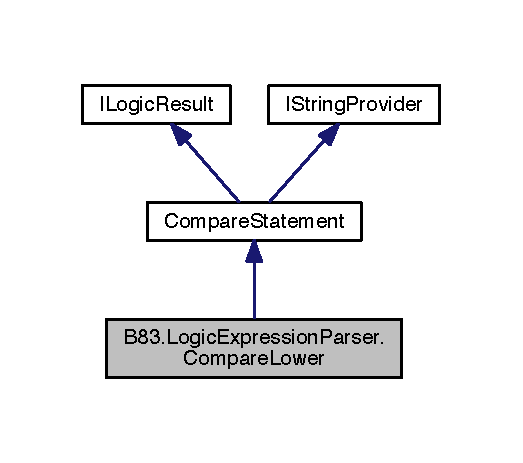
\includegraphics[width=251pt]{class_b83_1_1_logic_expression_parser_1_1_compare_lower__inherit__graph}
\end{center}
\end{figure}


Collaboration diagram for B83.\+Logic\+Expression\+Parser.\+Compare\+Lower\+:\nopagebreak
\begin{figure}[H]
\begin{center}
\leavevmode
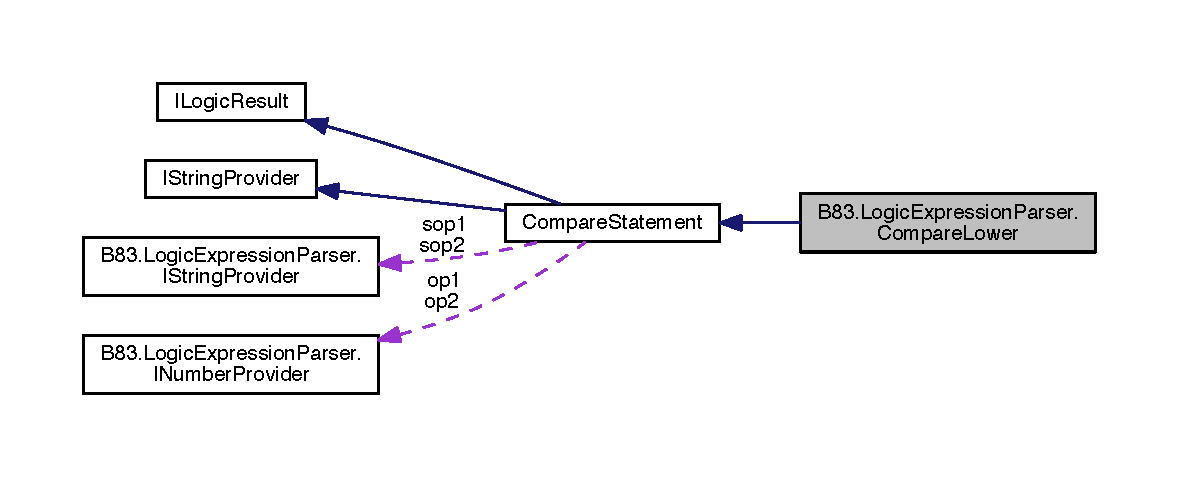
\includegraphics[width=350pt]{class_b83_1_1_logic_expression_parser_1_1_compare_lower__coll__graph}
\end{center}
\end{figure}
\subsection*{Protected Member Functions}
\begin{DoxyCompactItemize}
\item 
override bool {\bfseries Compare} (double a\+Op1, double a\+Op2)\hypertarget{class_b83_1_1_logic_expression_parser_1_1_compare_lower_a56c2c88ce62694ddc2ef1ebc6f9f85f3}{}\label{class_b83_1_1_logic_expression_parser_1_1_compare_lower_a56c2c88ce62694ddc2ef1ebc6f9f85f3}

\item 
override bool {\bfseries Compare} (string a\+Op1, string a\+Op2)\hypertarget{class_b83_1_1_logic_expression_parser_1_1_compare_lower_accd7611b66fefaffe118114794f00425}{}\label{class_b83_1_1_logic_expression_parser_1_1_compare_lower_accd7611b66fefaffe118114794f00425}

\end{DoxyCompactItemize}
\subsection*{Additional Inherited Members}


The documentation for this class was generated from the following file\+:\begin{DoxyCompactItemize}
\item 
/\+Users/pjd37/\+Documents/\+Git\+Hub/\+Blood\+Transfusion/\+B\+T/\+Assets/\+Scripts/Expr\+Test.\+cs\end{DoxyCompactItemize}

\hypertarget{class_b83_1_1_logic_expression_parser_1_1_compare_lower_or_equal}{}\section{B83.\+Logic\+Expression\+Parser.\+Compare\+Lower\+Or\+Equal Class Reference}
\label{class_b83_1_1_logic_expression_parser_1_1_compare_lower_or_equal}\index{B83.\+Logic\+Expression\+Parser.\+Compare\+Lower\+Or\+Equal@{B83.\+Logic\+Expression\+Parser.\+Compare\+Lower\+Or\+Equal}}


Inheritance diagram for B83.\+Logic\+Expression\+Parser.\+Compare\+Lower\+Or\+Equal\+:\nopagebreak
\begin{figure}[H]
\begin{center}
\leavevmode
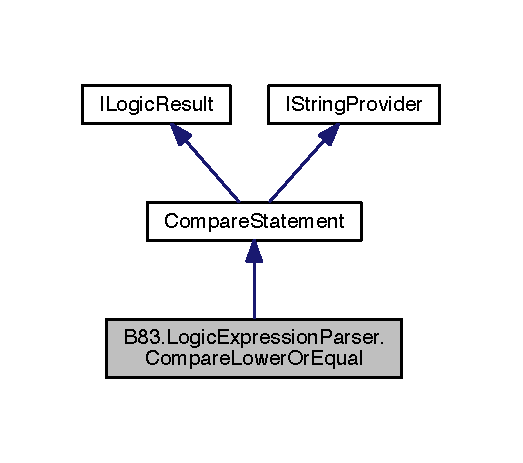
\includegraphics[width=251pt]{class_b83_1_1_logic_expression_parser_1_1_compare_lower_or_equal__inherit__graph}
\end{center}
\end{figure}


Collaboration diagram for B83.\+Logic\+Expression\+Parser.\+Compare\+Lower\+Or\+Equal\+:\nopagebreak
\begin{figure}[H]
\begin{center}
\leavevmode
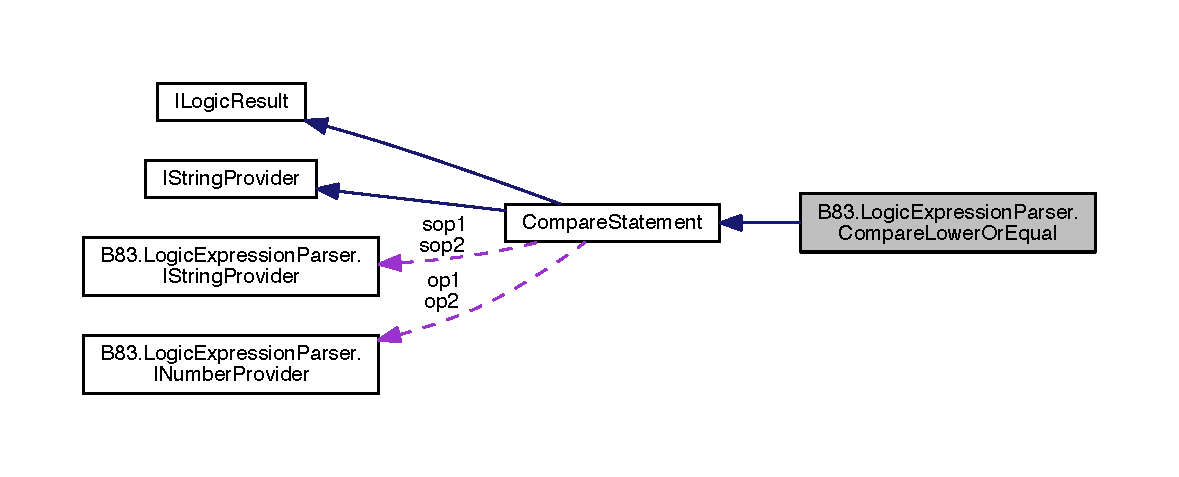
\includegraphics[width=350pt]{class_b83_1_1_logic_expression_parser_1_1_compare_lower_or_equal__coll__graph}
\end{center}
\end{figure}
\subsection*{Protected Member Functions}
\begin{DoxyCompactItemize}
\item 
override bool {\bfseries Compare} (double a\+Op1, double a\+Op2)\hypertarget{class_b83_1_1_logic_expression_parser_1_1_compare_lower_or_equal_a89f2fad109558a791d3319606a37ede0}{}\label{class_b83_1_1_logic_expression_parser_1_1_compare_lower_or_equal_a89f2fad109558a791d3319606a37ede0}

\item 
override bool {\bfseries Compare} (string a\+Op1, string a\+Op2)\hypertarget{class_b83_1_1_logic_expression_parser_1_1_compare_lower_or_equal_a5818b0f930b978cb0226fcdd6a08f8f4}{}\label{class_b83_1_1_logic_expression_parser_1_1_compare_lower_or_equal_a5818b0f930b978cb0226fcdd6a08f8f4}

\end{DoxyCompactItemize}
\subsection*{Additional Inherited Members}


The documentation for this class was generated from the following file\+:\begin{DoxyCompactItemize}
\item 
/\+Users/pjd37/\+Documents/\+Git\+Hub/\+Blood\+Transfusion/\+B\+T/\+Assets/\+Scripts/Expr\+Test.\+cs\end{DoxyCompactItemize}

\hypertarget{class_b83_1_1_logic_expression_parser_1_1_compare_not_equal}{}\section{B83.\+Logic\+Expression\+Parser.\+Compare\+Not\+Equal Class Reference}
\label{class_b83_1_1_logic_expression_parser_1_1_compare_not_equal}\index{B83.\+Logic\+Expression\+Parser.\+Compare\+Not\+Equal@{B83.\+Logic\+Expression\+Parser.\+Compare\+Not\+Equal}}


Inheritance diagram for B83.\+Logic\+Expression\+Parser.\+Compare\+Not\+Equal\+:\nopagebreak
\begin{figure}[H]
\begin{center}
\leavevmode
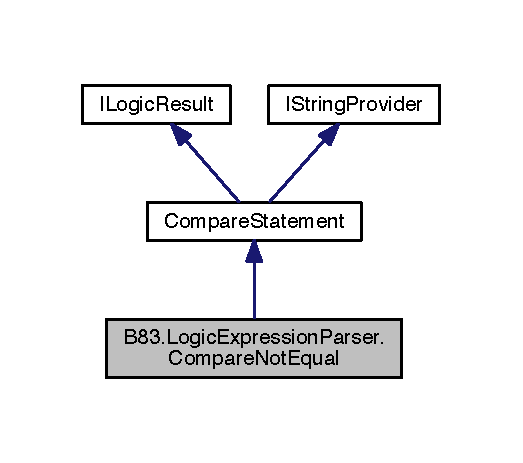
\includegraphics[width=251pt]{class_b83_1_1_logic_expression_parser_1_1_compare_not_equal__inherit__graph}
\end{center}
\end{figure}


Collaboration diagram for B83.\+Logic\+Expression\+Parser.\+Compare\+Not\+Equal\+:\nopagebreak
\begin{figure}[H]
\begin{center}
\leavevmode
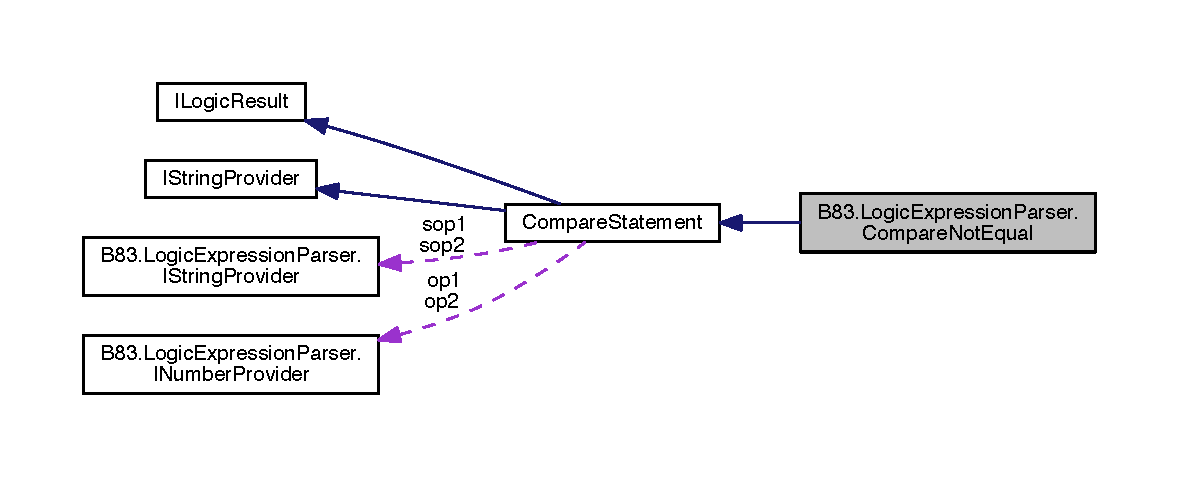
\includegraphics[width=350pt]{class_b83_1_1_logic_expression_parser_1_1_compare_not_equal__coll__graph}
\end{center}
\end{figure}
\subsection*{Protected Member Functions}
\begin{DoxyCompactItemize}
\item 
override bool {\bfseries Compare} (double a\+Op1, double a\+Op2)\hypertarget{class_b83_1_1_logic_expression_parser_1_1_compare_not_equal_a34dc8702ed0718bfda82877d331a3d58}{}\label{class_b83_1_1_logic_expression_parser_1_1_compare_not_equal_a34dc8702ed0718bfda82877d331a3d58}

\item 
override bool {\bfseries Compare} (string a\+Op1, string a\+Op2)\hypertarget{class_b83_1_1_logic_expression_parser_1_1_compare_not_equal_ad8098632ed8e385caba30f32f30705bc}{}\label{class_b83_1_1_logic_expression_parser_1_1_compare_not_equal_ad8098632ed8e385caba30f32f30705bc}

\end{DoxyCompactItemize}
\subsection*{Additional Inherited Members}


The documentation for this class was generated from the following file\+:\begin{DoxyCompactItemize}
\item 
/\+Users/pjd37/\+Documents/\+Git\+Hub/\+Blood\+Transfusion/\+B\+T/\+Assets/\+Scripts/Expr\+Test.\+cs\end{DoxyCompactItemize}

\hypertarget{class_b83_1_1_logic_expression_parser_1_1_compare_statement}{}\section{B83.\+Logic\+Expression\+Parser.\+Compare\+Statement Class Reference}
\label{class_b83_1_1_logic_expression_parser_1_1_compare_statement}\index{B83.\+Logic\+Expression\+Parser.\+Compare\+Statement@{B83.\+Logic\+Expression\+Parser.\+Compare\+Statement}}


Inheritance diagram for B83.\+Logic\+Expression\+Parser.\+Compare\+Statement\+:\nopagebreak
\begin{figure}[H]
\begin{center}
\leavevmode
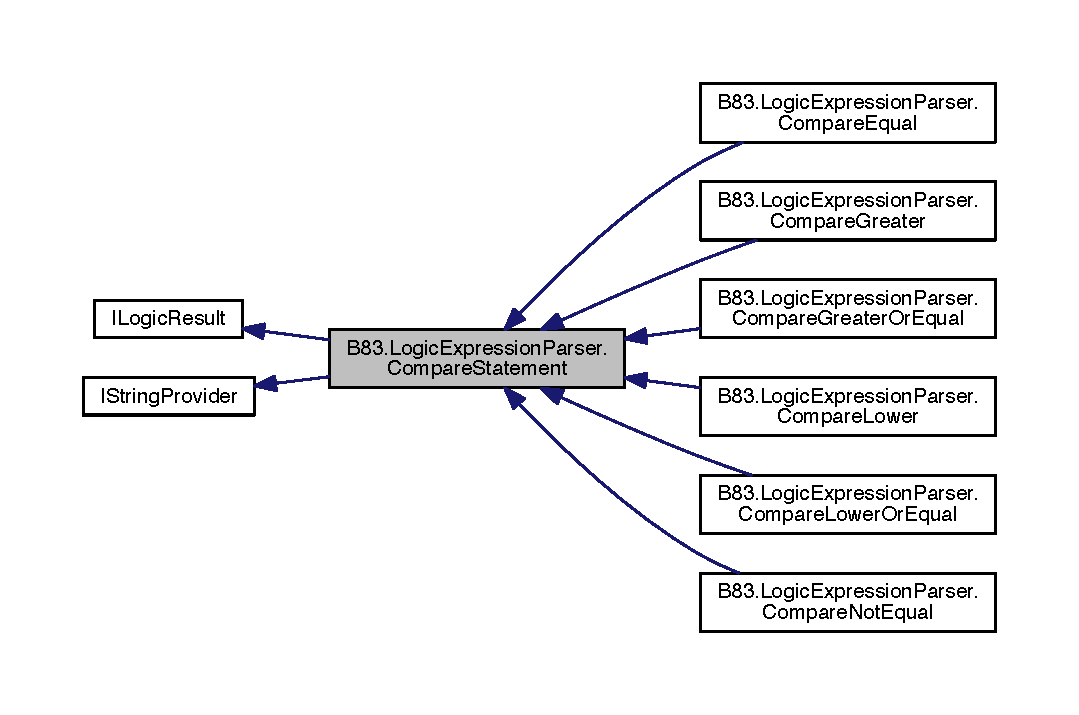
\includegraphics[width=350pt]{class_b83_1_1_logic_expression_parser_1_1_compare_statement__inherit__graph}
\end{center}
\end{figure}


Collaboration diagram for B83.\+Logic\+Expression\+Parser.\+Compare\+Statement\+:\nopagebreak
\begin{figure}[H]
\begin{center}
\leavevmode
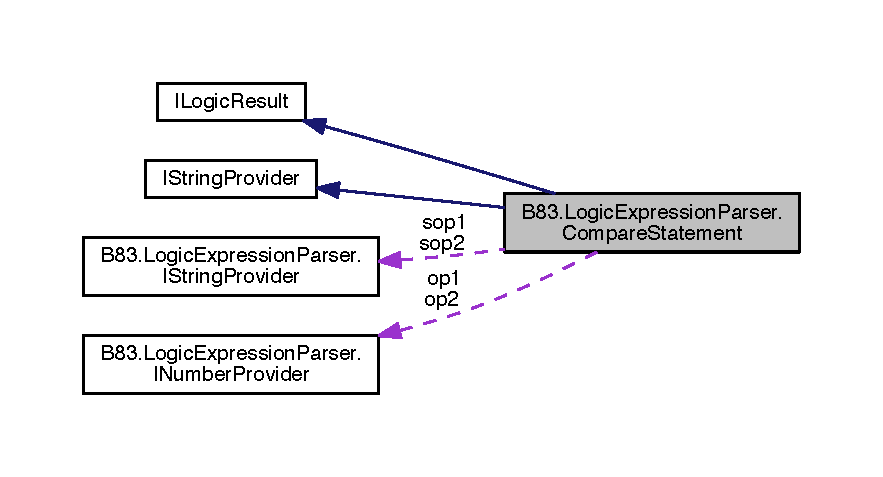
\includegraphics[width=350pt]{class_b83_1_1_logic_expression_parser_1_1_compare_statement__coll__graph}
\end{center}
\end{figure}
\subsection*{Public Member Functions}
\begin{DoxyCompactItemize}
\item 
bool {\bfseries Get\+Result} ()\hypertarget{class_b83_1_1_logic_expression_parser_1_1_compare_statement_ace01a17543b2605a9dd36d4a0bd441f5}{}\label{class_b83_1_1_logic_expression_parser_1_1_compare_statement_ace01a17543b2605a9dd36d4a0bd441f5}

\item 
string {\bfseries Get\+String} ()\hypertarget{class_b83_1_1_logic_expression_parser_1_1_compare_statement_a422a3629f04882c2b064c9a7042b7662}{}\label{class_b83_1_1_logic_expression_parser_1_1_compare_statement_a422a3629f04882c2b064c9a7042b7662}

\end{DoxyCompactItemize}
\subsection*{Public Attributes}
\begin{DoxyCompactItemize}
\item 
\hyperlink{interface_b83_1_1_logic_expression_parser_1_1_i_number_provider}{I\+Number\+Provider} {\bfseries op1}\hypertarget{class_b83_1_1_logic_expression_parser_1_1_compare_statement_a0136174967faf7192317de5807ebc7c4}{}\label{class_b83_1_1_logic_expression_parser_1_1_compare_statement_a0136174967faf7192317de5807ebc7c4}

\item 
\hyperlink{interface_b83_1_1_logic_expression_parser_1_1_i_number_provider}{I\+Number\+Provider} {\bfseries op2}\hypertarget{class_b83_1_1_logic_expression_parser_1_1_compare_statement_aad334a9d0f6dc79bc8994998b7f82294}{}\label{class_b83_1_1_logic_expression_parser_1_1_compare_statement_aad334a9d0f6dc79bc8994998b7f82294}

\item 
\hyperlink{interface_b83_1_1_logic_expression_parser_1_1_i_string_provider}{I\+String\+Provider} {\bfseries sop1}\hypertarget{class_b83_1_1_logic_expression_parser_1_1_compare_statement_acb4ed8c53dcb43a57e4fcc7c13c5d580}{}\label{class_b83_1_1_logic_expression_parser_1_1_compare_statement_acb4ed8c53dcb43a57e4fcc7c13c5d580}

\item 
\hyperlink{interface_b83_1_1_logic_expression_parser_1_1_i_string_provider}{I\+String\+Provider} {\bfseries sop2}\hypertarget{class_b83_1_1_logic_expression_parser_1_1_compare_statement_a95c19539d32e65e6cb1e0e5293811f83}{}\label{class_b83_1_1_logic_expression_parser_1_1_compare_statement_a95c19539d32e65e6cb1e0e5293811f83}

\end{DoxyCompactItemize}
\subsection*{Protected Member Functions}
\begin{DoxyCompactItemize}
\item 
abstract bool {\bfseries Compare} (double a\+Op1, double a\+Op2)\hypertarget{class_b83_1_1_logic_expression_parser_1_1_compare_statement_a94ee275c1487f33c70178242a643be40}{}\label{class_b83_1_1_logic_expression_parser_1_1_compare_statement_a94ee275c1487f33c70178242a643be40}

\item 
abstract bool {\bfseries Compare} (string a\+Op1, string a\+Op2)\hypertarget{class_b83_1_1_logic_expression_parser_1_1_compare_statement_a81c5449e336fec9fd3bd3a398be2f402}{}\label{class_b83_1_1_logic_expression_parser_1_1_compare_statement_a81c5449e336fec9fd3bd3a398be2f402}

\end{DoxyCompactItemize}


The documentation for this class was generated from the following file\+:\begin{DoxyCompactItemize}
\item 
/\+Users/pjd37/\+Documents/\+Git\+Hub/\+Blood\+Transfusion/\+B\+T/\+Assets/\+Scripts/Expr\+Test.\+cs\end{DoxyCompactItemize}

\hypertarget{class_b83_1_1_logic_expression_parser_1_1_constant_bool}{}\section{B83.\+Logic\+Expression\+Parser.\+Constant\+Bool Class Reference}
\label{class_b83_1_1_logic_expression_parser_1_1_constant_bool}\index{B83.\+Logic\+Expression\+Parser.\+Constant\+Bool@{B83.\+Logic\+Expression\+Parser.\+Constant\+Bool}}


Inheritance diagram for B83.\+Logic\+Expression\+Parser.\+Constant\+Bool\+:\nopagebreak
\begin{figure}[H]
\begin{center}
\leavevmode
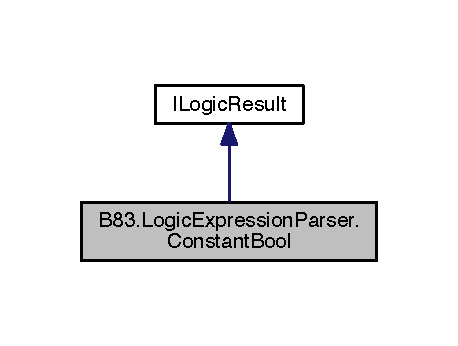
\includegraphics[width=220pt]{class_b83_1_1_logic_expression_parser_1_1_constant_bool__inherit__graph}
\end{center}
\end{figure}


Collaboration diagram for B83.\+Logic\+Expression\+Parser.\+Constant\+Bool\+:\nopagebreak
\begin{figure}[H]
\begin{center}
\leavevmode
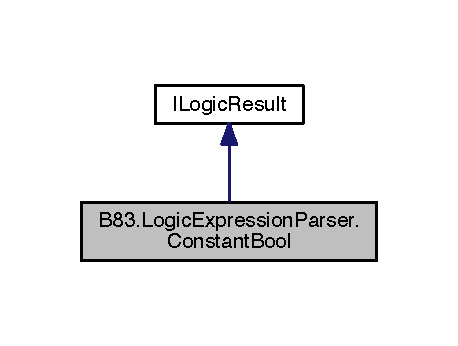
\includegraphics[width=220pt]{class_b83_1_1_logic_expression_parser_1_1_constant_bool__coll__graph}
\end{center}
\end{figure}
\subsection*{Public Member Functions}
\begin{DoxyCompactItemize}
\item 
bool {\bfseries Get\+Result} ()\hypertarget{class_b83_1_1_logic_expression_parser_1_1_constant_bool_a8eaa6a2f3a9ee1f02e0ac156517ec69c}{}\label{class_b83_1_1_logic_expression_parser_1_1_constant_bool_a8eaa6a2f3a9ee1f02e0ac156517ec69c}

\end{DoxyCompactItemize}
\subsection*{Public Attributes}
\begin{DoxyCompactItemize}
\item 
bool {\bfseries constant\+Value}\hypertarget{class_b83_1_1_logic_expression_parser_1_1_constant_bool_ac4ddaec7c5f46361e3277494cdf244bb}{}\label{class_b83_1_1_logic_expression_parser_1_1_constant_bool_ac4ddaec7c5f46361e3277494cdf244bb}

\end{DoxyCompactItemize}


The documentation for this class was generated from the following file\+:\begin{DoxyCompactItemize}
\item 
/\+Users/pjd37/\+Documents/\+Git\+Hub/\+Blood\+Transfusion/\+B\+T/\+Assets/\+Scripts/Expr\+Test.\+cs\end{DoxyCompactItemize}

\hypertarget{class_b83_1_1_logic_expression_parser_1_1_constant_number}{}\section{B83.\+Logic\+Expression\+Parser.\+Constant\+Number Class Reference}
\label{class_b83_1_1_logic_expression_parser_1_1_constant_number}\index{B83.\+Logic\+Expression\+Parser.\+Constant\+Number@{B83.\+Logic\+Expression\+Parser.\+Constant\+Number}}


Inheritance diagram for B83.\+Logic\+Expression\+Parser.\+Constant\+Number\+:\nopagebreak
\begin{figure}[H]
\begin{center}
\leavevmode
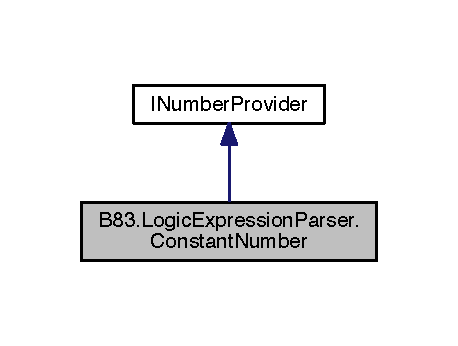
\includegraphics[width=220pt]{class_b83_1_1_logic_expression_parser_1_1_constant_number__inherit__graph}
\end{center}
\end{figure}


Collaboration diagram for B83.\+Logic\+Expression\+Parser.\+Constant\+Number\+:\nopagebreak
\begin{figure}[H]
\begin{center}
\leavevmode
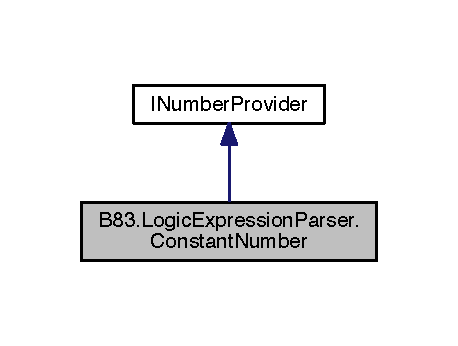
\includegraphics[width=220pt]{class_b83_1_1_logic_expression_parser_1_1_constant_number__coll__graph}
\end{center}
\end{figure}
\subsection*{Public Member Functions}
\begin{DoxyCompactItemize}
\item 
double {\bfseries Get\+Number} ()\hypertarget{class_b83_1_1_logic_expression_parser_1_1_constant_number_a043c02f32ca78c75fa3d483385d5dc86}{}\label{class_b83_1_1_logic_expression_parser_1_1_constant_number_a043c02f32ca78c75fa3d483385d5dc86}

\item 
bool {\bfseries Is\+String} ()\hypertarget{class_b83_1_1_logic_expression_parser_1_1_constant_number_ad4c8f2ce0a36408bbaddae052f9c610a}{}\label{class_b83_1_1_logic_expression_parser_1_1_constant_number_ad4c8f2ce0a36408bbaddae052f9c610a}

\end{DoxyCompactItemize}
\subsection*{Public Attributes}
\begin{DoxyCompactItemize}
\item 
double {\bfseries constant\+Value}\hypertarget{class_b83_1_1_logic_expression_parser_1_1_constant_number_a56bd2dea115625bb179f9cc14d7ab29a}{}\label{class_b83_1_1_logic_expression_parser_1_1_constant_number_a56bd2dea115625bb179f9cc14d7ab29a}

\item 
bool {\bfseries is\+String} = false\hypertarget{class_b83_1_1_logic_expression_parser_1_1_constant_number_acfa7789cf1eb7339338cc6f712009013}{}\label{class_b83_1_1_logic_expression_parser_1_1_constant_number_acfa7789cf1eb7339338cc6f712009013}

\end{DoxyCompactItemize}


The documentation for this class was generated from the following file\+:\begin{DoxyCompactItemize}
\item 
/\+Users/pjd37/\+Documents/\+Git\+Hub/\+Blood\+Transfusion/\+B\+T/\+Assets/\+Scripts/Expr\+Test.\+cs\end{DoxyCompactItemize}

\hypertarget{class_b83_1_1_logic_expression_parser_1_1_constant_string}{}\section{B83.\+Logic\+Expression\+Parser.\+Constant\+String Class Reference}
\label{class_b83_1_1_logic_expression_parser_1_1_constant_string}\index{B83.\+Logic\+Expression\+Parser.\+Constant\+String@{B83.\+Logic\+Expression\+Parser.\+Constant\+String}}


Inheritance diagram for B83.\+Logic\+Expression\+Parser.\+Constant\+String\+:\nopagebreak
\begin{figure}[H]
\begin{center}
\leavevmode
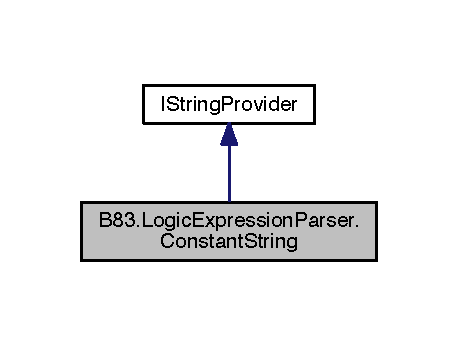
\includegraphics[width=220pt]{class_b83_1_1_logic_expression_parser_1_1_constant_string__inherit__graph}
\end{center}
\end{figure}


Collaboration diagram for B83.\+Logic\+Expression\+Parser.\+Constant\+String\+:\nopagebreak
\begin{figure}[H]
\begin{center}
\leavevmode
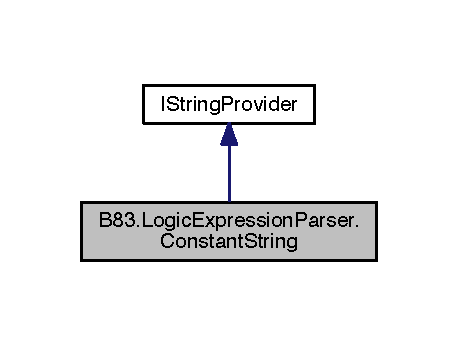
\includegraphics[width=220pt]{class_b83_1_1_logic_expression_parser_1_1_constant_string__coll__graph}
\end{center}
\end{figure}
\subsection*{Public Member Functions}
\begin{DoxyCompactItemize}
\item 
string {\bfseries Get\+String} ()\hypertarget{class_b83_1_1_logic_expression_parser_1_1_constant_string_a35dec11c978c70df1bc7f5346e55ecea}{}\label{class_b83_1_1_logic_expression_parser_1_1_constant_string_a35dec11c978c70df1bc7f5346e55ecea}

\end{DoxyCompactItemize}
\subsection*{Public Attributes}
\begin{DoxyCompactItemize}
\item 
string {\bfseries constant\+Value}\hypertarget{class_b83_1_1_logic_expression_parser_1_1_constant_string_a1ff502a70aa863e44844627300a81b54}{}\label{class_b83_1_1_logic_expression_parser_1_1_constant_string_a1ff502a70aa863e44844627300a81b54}

\end{DoxyCompactItemize}


The documentation for this class was generated from the following file\+:\begin{DoxyCompactItemize}
\item 
/\+Users/pjd37/\+Documents/\+Git\+Hub/\+Blood\+Transfusion/\+B\+T/\+Assets/\+Scripts/Expr\+Test.\+cs\end{DoxyCompactItemize}

\hypertarget{class_b83_1_1_logic_expression_parser_1_1_custom_function}{}\section{B83.\+Logic\+Expression\+Parser.\+Custom\+Function Class Reference}
\label{class_b83_1_1_logic_expression_parser_1_1_custom_function}\index{B83.\+Logic\+Expression\+Parser.\+Custom\+Function@{B83.\+Logic\+Expression\+Parser.\+Custom\+Function}}


Inheritance diagram for B83.\+Logic\+Expression\+Parser.\+Custom\+Function\+:\nopagebreak
\begin{figure}[H]
\begin{center}
\leavevmode
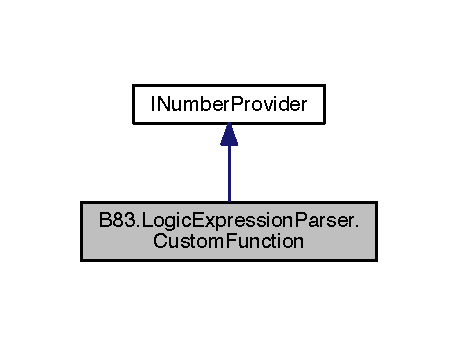
\includegraphics[width=220pt]{class_b83_1_1_logic_expression_parser_1_1_custom_function__inherit__graph}
\end{center}
\end{figure}


Collaboration diagram for B83.\+Logic\+Expression\+Parser.\+Custom\+Function\+:\nopagebreak
\begin{figure}[H]
\begin{center}
\leavevmode
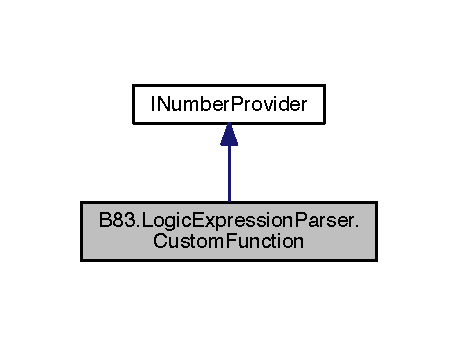
\includegraphics[width=220pt]{class_b83_1_1_logic_expression_parser_1_1_custom_function__coll__graph}
\end{center}
\end{figure}
\subsection*{Public Member Functions}
\begin{DoxyCompactItemize}
\item 
{\bfseries Custom\+Function} (Func$<$ \hyperlink{class_b83_1_1_logic_expression_parser_1_1_parameter_list}{Parameter\+List}, double $>$ a\+Func, \hyperlink{class_b83_1_1_logic_expression_parser_1_1_parameter_list}{Parameter\+List} a\+Params)\hypertarget{class_b83_1_1_logic_expression_parser_1_1_custom_function_a3439217b747e65290fb4c00ad1cfe8b6}{}\label{class_b83_1_1_logic_expression_parser_1_1_custom_function_a3439217b747e65290fb4c00ad1cfe8b6}

\item 
bool {\bfseries Is\+String} ()\hypertarget{class_b83_1_1_logic_expression_parser_1_1_custom_function_ade89d1c0f4c28c5a287f3488ed3ee1da}{}\label{class_b83_1_1_logic_expression_parser_1_1_custom_function_ade89d1c0f4c28c5a287f3488ed3ee1da}

\item 
double {\bfseries Get\+Number} ()\hypertarget{class_b83_1_1_logic_expression_parser_1_1_custom_function_ac05287f07b73df30ab2e6c8a968e6b49}{}\label{class_b83_1_1_logic_expression_parser_1_1_custom_function_ac05287f07b73df30ab2e6c8a968e6b49}

\end{DoxyCompactItemize}


The documentation for this class was generated from the following file\+:\begin{DoxyCompactItemize}
\item 
/\+Users/pjd37/\+Documents/\+Git\+Hub/\+Blood\+Transfusion/\+B\+T/\+Assets/\+Scripts/Expr\+Test.\+cs\end{DoxyCompactItemize}

\hypertarget{class_b83_1_1_logic_expression_parser_1_1_custom_string_function}{}\section{B83.\+Logic\+Expression\+Parser.\+Custom\+String\+Function Class Reference}
\label{class_b83_1_1_logic_expression_parser_1_1_custom_string_function}\index{B83.\+Logic\+Expression\+Parser.\+Custom\+String\+Function@{B83.\+Logic\+Expression\+Parser.\+Custom\+String\+Function}}


Inheritance diagram for B83.\+Logic\+Expression\+Parser.\+Custom\+String\+Function\+:\nopagebreak
\begin{figure}[H]
\begin{center}
\leavevmode
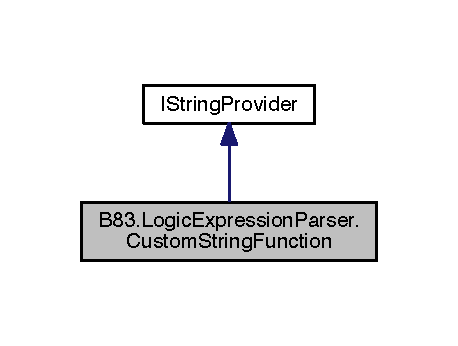
\includegraphics[width=220pt]{class_b83_1_1_logic_expression_parser_1_1_custom_string_function__inherit__graph}
\end{center}
\end{figure}


Collaboration diagram for B83.\+Logic\+Expression\+Parser.\+Custom\+String\+Function\+:\nopagebreak
\begin{figure}[H]
\begin{center}
\leavevmode
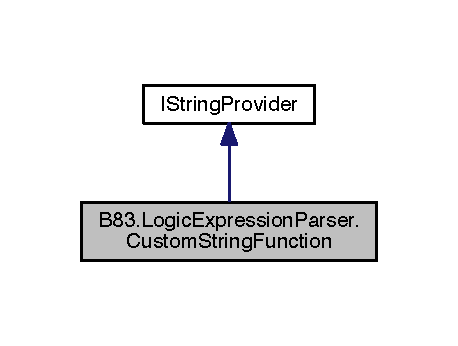
\includegraphics[width=220pt]{class_b83_1_1_logic_expression_parser_1_1_custom_string_function__coll__graph}
\end{center}
\end{figure}
\subsection*{Public Member Functions}
\begin{DoxyCompactItemize}
\item 
void {\bfseries Custom\+Function} (Func$<$ \hyperlink{class_b83_1_1_logic_expression_parser_1_1_parameter_list}{Parameter\+List}, string $>$ a\+Func, \hyperlink{class_b83_1_1_logic_expression_parser_1_1_parameter_list}{Parameter\+List} a\+Params)\hypertarget{class_b83_1_1_logic_expression_parser_1_1_custom_string_function_ad0e16499b68791f36429fd99b370251f}{}\label{class_b83_1_1_logic_expression_parser_1_1_custom_string_function_ad0e16499b68791f36429fd99b370251f}

\item 
string {\bfseries Get\+String} ()\hypertarget{class_b83_1_1_logic_expression_parser_1_1_custom_string_function_a4bd29c84c65faec0a3cb415a3ca3e06a}{}\label{class_b83_1_1_logic_expression_parser_1_1_custom_string_function_a4bd29c84c65faec0a3cb415a3ca3e06a}

\end{DoxyCompactItemize}


The documentation for this class was generated from the following file\+:\begin{DoxyCompactItemize}
\item 
/\+Users/pjd37/\+Documents/\+Git\+Hub/\+Blood\+Transfusion/\+B\+T/\+Assets/\+Scripts/Expr\+Test.\+cs\end{DoxyCompactItemize}

\hypertarget{class_b83_1_1_logic_expression_parser_1_1_delegate_bool}{}\section{B83.\+Logic\+Expression\+Parser.\+Delegate\+Bool Class Reference}
\label{class_b83_1_1_logic_expression_parser_1_1_delegate_bool}\index{B83.\+Logic\+Expression\+Parser.\+Delegate\+Bool@{B83.\+Logic\+Expression\+Parser.\+Delegate\+Bool}}


Inheritance diagram for B83.\+Logic\+Expression\+Parser.\+Delegate\+Bool\+:\nopagebreak
\begin{figure}[H]
\begin{center}
\leavevmode
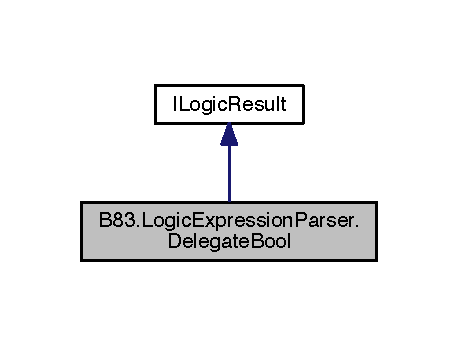
\includegraphics[width=220pt]{class_b83_1_1_logic_expression_parser_1_1_delegate_bool__inherit__graph}
\end{center}
\end{figure}


Collaboration diagram for B83.\+Logic\+Expression\+Parser.\+Delegate\+Bool\+:\nopagebreak
\begin{figure}[H]
\begin{center}
\leavevmode
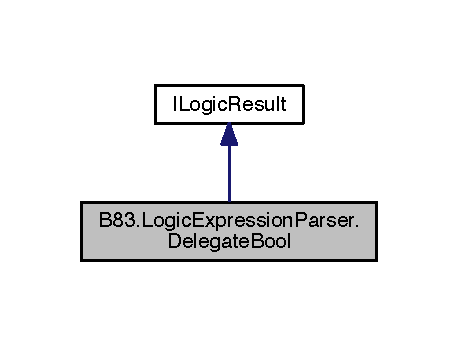
\includegraphics[width=220pt]{class_b83_1_1_logic_expression_parser_1_1_delegate_bool__coll__graph}
\end{center}
\end{figure}
\subsection*{Public Member Functions}
\begin{DoxyCompactItemize}
\item 
bool {\bfseries Get\+Result} ()\hypertarget{class_b83_1_1_logic_expression_parser_1_1_delegate_bool_a89ee2921ce6153017d8f1a0f98cc5e23}{}\label{class_b83_1_1_logic_expression_parser_1_1_delegate_bool_a89ee2921ce6153017d8f1a0f98cc5e23}

\end{DoxyCompactItemize}
\subsection*{Public Attributes}
\begin{DoxyCompactItemize}
\item 
Func$<$ bool $>$ {\bfseries callback}\hypertarget{class_b83_1_1_logic_expression_parser_1_1_delegate_bool_ab01aef9adb9394f583cb8347bd3d9b44}{}\label{class_b83_1_1_logic_expression_parser_1_1_delegate_bool_ab01aef9adb9394f583cb8347bd3d9b44}

\end{DoxyCompactItemize}


The documentation for this class was generated from the following file\+:\begin{DoxyCompactItemize}
\item 
/\+Users/pjd37/\+Documents/\+Git\+Hub/\+Blood\+Transfusion/\+B\+T/\+Assets/\+Scripts/Expr\+Test.\+cs\end{DoxyCompactItemize}

\hypertarget{class_b83_1_1_logic_expression_parser_1_1_delegate_number}{}\section{B83.\+Logic\+Expression\+Parser.\+Delegate\+Number Class Reference}
\label{class_b83_1_1_logic_expression_parser_1_1_delegate_number}\index{B83.\+Logic\+Expression\+Parser.\+Delegate\+Number@{B83.\+Logic\+Expression\+Parser.\+Delegate\+Number}}


Inheritance diagram for B83.\+Logic\+Expression\+Parser.\+Delegate\+Number\+:\nopagebreak
\begin{figure}[H]
\begin{center}
\leavevmode
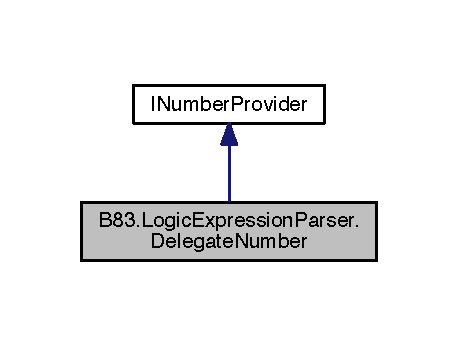
\includegraphics[width=220pt]{class_b83_1_1_logic_expression_parser_1_1_delegate_number__inherit__graph}
\end{center}
\end{figure}


Collaboration diagram for B83.\+Logic\+Expression\+Parser.\+Delegate\+Number\+:\nopagebreak
\begin{figure}[H]
\begin{center}
\leavevmode
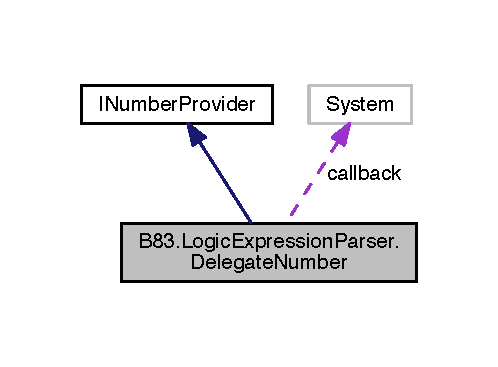
\includegraphics[width=239pt]{class_b83_1_1_logic_expression_parser_1_1_delegate_number__coll__graph}
\end{center}
\end{figure}
\subsection*{Public Member Functions}
\begin{DoxyCompactItemize}
\item 
bool {\bfseries Is\+String} ()\hypertarget{class_b83_1_1_logic_expression_parser_1_1_delegate_number_aa4a76a979703bad92eb54923bd03ee94}{}\label{class_b83_1_1_logic_expression_parser_1_1_delegate_number_aa4a76a979703bad92eb54923bd03ee94}

\item 
double {\bfseries Get\+Number} ()\hypertarget{class_b83_1_1_logic_expression_parser_1_1_delegate_number_aef1f9121b9a10bc5815379d6fb86c825}{}\label{class_b83_1_1_logic_expression_parser_1_1_delegate_number_aef1f9121b9a10bc5815379d6fb86c825}

\end{DoxyCompactItemize}
\subsection*{Public Attributes}
\begin{DoxyCompactItemize}
\item 
System.\+Func$<$ double $>$ {\bfseries callback}\hypertarget{class_b83_1_1_logic_expression_parser_1_1_delegate_number_a9b536a4b068b2e215bb2269e2bc477a5}{}\label{class_b83_1_1_logic_expression_parser_1_1_delegate_number_a9b536a4b068b2e215bb2269e2bc477a5}

\end{DoxyCompactItemize}


The documentation for this class was generated from the following file\+:\begin{DoxyCompactItemize}
\item 
/\+Users/pjd37/\+Documents/\+Git\+Hub/\+Blood\+Transfusion/\+B\+T/\+Assets/\+Scripts/Expr\+Test.\+cs\end{DoxyCompactItemize}

\hypertarget{class_b83_1_1_logic_expression_parser_1_1_delegate_string}{}\section{B83.\+Logic\+Expression\+Parser.\+Delegate\+String Class Reference}
\label{class_b83_1_1_logic_expression_parser_1_1_delegate_string}\index{B83.\+Logic\+Expression\+Parser.\+Delegate\+String@{B83.\+Logic\+Expression\+Parser.\+Delegate\+String}}


Inheritance diagram for B83.\+Logic\+Expression\+Parser.\+Delegate\+String\+:\nopagebreak
\begin{figure}[H]
\begin{center}
\leavevmode
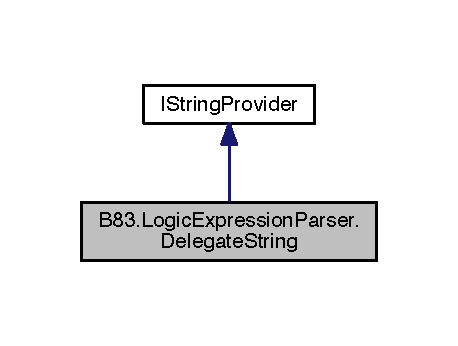
\includegraphics[width=220pt]{class_b83_1_1_logic_expression_parser_1_1_delegate_string__inherit__graph}
\end{center}
\end{figure}


Collaboration diagram for B83.\+Logic\+Expression\+Parser.\+Delegate\+String\+:\nopagebreak
\begin{figure}[H]
\begin{center}
\leavevmode
\includegraphics[width=233pt]{class_b83_1_1_logic_expression_parser_1_1_delegate_string__coll__graph}
\end{center}
\end{figure}
\subsection*{Public Member Functions}
\begin{DoxyCompactItemize}
\item 
string {\bfseries Get\+String} ()\hypertarget{class_b83_1_1_logic_expression_parser_1_1_delegate_string_a0543e6f7c89072b827dab4c9932bbe2c}{}\label{class_b83_1_1_logic_expression_parser_1_1_delegate_string_a0543e6f7c89072b827dab4c9932bbe2c}

\end{DoxyCompactItemize}
\subsection*{Public Attributes}
\begin{DoxyCompactItemize}
\item 
System.\+Func$<$ string $>$ {\bfseries callback}\hypertarget{class_b83_1_1_logic_expression_parser_1_1_delegate_string_a38adf113639aa2f2c564d3fd8d54cca2}{}\label{class_b83_1_1_logic_expression_parser_1_1_delegate_string_a38adf113639aa2f2c564d3fd8d54cca2}

\end{DoxyCompactItemize}


The documentation for this class was generated from the following file\+:\begin{DoxyCompactItemize}
\item 
/\+Users/pjd37/\+Documents/\+Git\+Hub/\+Blood\+Transfusion/\+B\+T/\+Assets/\+Scripts/Expr\+Test.\+cs\end{DoxyCompactItemize}

\hypertarget{class_b83_1_1_logic_expression_parser_1_1_expression_context}{}\section{B83.\+Logic\+Expression\+Parser.\+Expression\+Context Class Reference}
\label{class_b83_1_1_logic_expression_parser_1_1_expression_context}\index{B83.\+Logic\+Expression\+Parser.\+Expression\+Context@{B83.\+Logic\+Expression\+Parser.\+Expression\+Context}}
\subsection*{Public Member Functions}
\begin{DoxyCompactItemize}
\item 
{\bfseries Expression\+Context} (bool a\+Add\+Default\+Constants)\hypertarget{class_b83_1_1_logic_expression_parser_1_1_expression_context_a87b31cf1e3bb8dfa521c27c1e2dfdd8a}{}\label{class_b83_1_1_logic_expression_parser_1_1_expression_context_a87b31cf1e3bb8dfa521c27c1e2dfdd8a}

\item 
void {\bfseries Add\+Math\+Constants} ()\hypertarget{class_b83_1_1_logic_expression_parser_1_1_expression_context_ae81739af37301a8855a899d13fd36345}{}\label{class_b83_1_1_logic_expression_parser_1_1_expression_context_ae81739af37301a8855a899d13fd36345}

\item 
virtual \hyperlink{class_b83_1_1_logic_expression_parser_1_1_expression_variable}{Expression\+Variable} {\bfseries Find\+Variable} (string a\+Var\+Name)\hypertarget{class_b83_1_1_logic_expression_parser_1_1_expression_context_a27a1c6d266599d39cf05d5ae30192d1e}{}\label{class_b83_1_1_logic_expression_parser_1_1_expression_context_a27a1c6d266599d39cf05d5ae30192d1e}

\item 
virtual \hyperlink{class_b83_1_1_logic_expression_parser_1_1_expression_variable}{Expression\+Variable} {\bfseries Get\+Variable} (string a\+Var\+Name)\hypertarget{class_b83_1_1_logic_expression_parser_1_1_expression_context_a5ca887a576d0f4471f42c125294ac56f}{}\label{class_b83_1_1_logic_expression_parser_1_1_expression_context_a5ca887a576d0f4471f42c125294ac56f}

\end{DoxyCompactItemize}
\subsection*{Protected Attributes}
\begin{DoxyCompactItemize}
\item 
Dictionary$<$ string, \hyperlink{class_b83_1_1_logic_expression_parser_1_1_expression_variable}{Expression\+Variable} $>$ {\bfseries variables} = new Dictionary$<$string, \hyperlink{class_b83_1_1_logic_expression_parser_1_1_expression_variable}{Expression\+Variable}$>$()\hypertarget{class_b83_1_1_logic_expression_parser_1_1_expression_context_a647e64f0cff08b7e158f0d53e652a18f}{}\label{class_b83_1_1_logic_expression_parser_1_1_expression_context_a647e64f0cff08b7e158f0d53e652a18f}

\end{DoxyCompactItemize}
\subsection*{Properties}
\begin{DoxyCompactItemize}
\item 
virtual \hyperlink{class_b83_1_1_logic_expression_parser_1_1_expression_variable}{Expression\+Variable} {\bfseries this\mbox{[}string a\+Var\+Name\mbox{]}}\hspace{0.3cm}{\ttfamily  \mbox{[}get\mbox{]}}\hypertarget{class_b83_1_1_logic_expression_parser_1_1_expression_context_ac03ce0e2bd5042641252937f778e1b1a}{}\label{class_b83_1_1_logic_expression_parser_1_1_expression_context_ac03ce0e2bd5042641252937f778e1b1a}

\end{DoxyCompactItemize}


The documentation for this class was generated from the following file\+:\begin{DoxyCompactItemize}
\item 
/\+Users/pjd37/\+Documents/\+Git\+Hub/\+Blood\+Transfusion/\+B\+T/\+Assets/\+Scripts/Expr\+Test.\+cs\end{DoxyCompactItemize}

\hypertarget{class_expression_parser}{}\section{Expression\+Parser Class Reference}
\label{class_expression_parser}\index{Expression\+Parser@{Expression\+Parser}}
\subsection*{Public Member Functions}
\begin{DoxyCompactItemize}
\item 
void {\bfseries Set\+Var} (string name, \hyperlink{class_param_data}{Param\+Data} value)\hypertarget{class_expression_parser_a5067e1c52821da4c67993e115eb3298e}{}\label{class_expression_parser_a5067e1c52821da4c67993e115eb3298e}

\item 
\hyperlink{class_param_data}{Param\+Data} {\bfseries Evaluate\+Param} (string expression)\hypertarget{class_expression_parser_a3a4c3b2b45de9270e163008462f39136}{}\label{class_expression_parser_a3a4c3b2b45de9270e163008462f39136}

\end{DoxyCompactItemize}


The documentation for this class was generated from the following file\+:\begin{DoxyCompactItemize}
\item 
/\+Users/pjd37/\+Documents/\+Git\+Hub/\+Blood\+Transfusion/\+B\+T/\+Assets/\+Scripts/My\+Game\+Manager.\+cs\end{DoxyCompactItemize}

\hypertarget{class_little_brain_1_1_g_m_addr_1_1_expression_parser}{}\section{Little\+Brain.\+G\+M\+Addr.\+Expression\+Parser Class Reference}
\label{class_little_brain_1_1_g_m_addr_1_1_expression_parser}\index{Little\+Brain.\+G\+M\+Addr.\+Expression\+Parser@{Little\+Brain.\+G\+M\+Addr.\+Expression\+Parser}}
\subsection*{Public Member Functions}
\begin{DoxyCompactItemize}
\item 
void {\bfseries Set\+Var} (string name, \hyperlink{class_little_brain_1_1_g_m_addr_1_1_param_data}{Param\+Data} value)\hypertarget{class_little_brain_1_1_g_m_addr_1_1_expression_parser_a9e2d027e9c2e4701540c5b6c049ef990}{}\label{class_little_brain_1_1_g_m_addr_1_1_expression_parser_a9e2d027e9c2e4701540c5b6c049ef990}

\item 
\hyperlink{class_little_brain_1_1_g_m_addr_1_1_param_data}{Param\+Data} {\bfseries Evaluate\+Param} (string expression)\hypertarget{class_little_brain_1_1_g_m_addr_1_1_expression_parser_a918f0c70f5365bafc1be74e3a098636c}{}\label{class_little_brain_1_1_g_m_addr_1_1_expression_parser_a918f0c70f5365bafc1be74e3a098636c}

\end{DoxyCompactItemize}
\subsection*{Public Attributes}
\begin{DoxyCompactItemize}
\item 
Data\+Table {\bfseries lo\+Data\+Table}\hypertarget{class_little_brain_1_1_g_m_addr_1_1_expression_parser_ad9f5194ee47eba569ba6862240316207}{}\label{class_little_brain_1_1_g_m_addr_1_1_expression_parser_ad9f5194ee47eba569ba6862240316207}

\item 
Data\+Type {\bfseries data\+Type}\hypertarget{class_little_brain_1_1_g_m_addr_1_1_expression_parser_ac454623360ed1ca699364f126abb2190}{}\label{class_little_brain_1_1_g_m_addr_1_1_expression_parser_ac454623360ed1ca699364f126abb2190}

\end{DoxyCompactItemize}


The documentation for this class was generated from the following file\+:\begin{DoxyCompactItemize}
\item 
/\+Users/pjd37/\+Documents/\+Git\+Hub/\+Blood\+Transfusion/\+B\+T/\+Assets/\+Scripts/My\+Game\+Manager\+Addr.\+cs\end{DoxyCompactItemize}

\hypertarget{class_expression_parser_d_t}{}\section{Expression\+Parser\+DT Class Reference}
\label{class_expression_parser_d_t}\index{Expression\+Parser\+DT@{Expression\+Parser\+DT}}
\subsection*{Public Member Functions}
\begin{DoxyCompactItemize}
\item 
void {\bfseries Set\+Var} (string name, \hyperlink{class_param_data}{Param\+Data} value)\hypertarget{class_expression_parser_d_t_afb79789782db3253ec2b5b54a042834f}{}\label{class_expression_parser_d_t_afb79789782db3253ec2b5b54a042834f}

\item 
\hyperlink{class_param_data}{Param\+Data} {\bfseries Evaluate\+Param} (string expression)\hypertarget{class_expression_parser_d_t_ab73e5422254a83bb4ccd9f746ea84cc2}{}\label{class_expression_parser_d_t_ab73e5422254a83bb4ccd9f746ea84cc2}

\end{DoxyCompactItemize}
\subsection*{Public Attributes}
\begin{DoxyCompactItemize}
\item 
Data\+Table {\bfseries lo\+Data\+Table}\hypertarget{class_expression_parser_d_t_abd243e927c9d496088821dac61086868}{}\label{class_expression_parser_d_t_abd243e927c9d496088821dac61086868}

\item 
Data\+Type {\bfseries data\+Type}\hypertarget{class_expression_parser_d_t_a9199550fe6c2f63f7f7710d7f8fb8972}{}\label{class_expression_parser_d_t_a9199550fe6c2f63f7f7710d7f8fb8972}

\end{DoxyCompactItemize}


The documentation for this class was generated from the following file\+:\begin{DoxyCompactItemize}
\item 
/\+Users/pjd37/\+Documents/\+Git\+Hub/\+Blood\+Transfusion/\+B\+T/\+Assets/\+Scripts/My\+Game\+Manager.\+cs\end{DoxyCompactItemize}

\hypertarget{class_b83_1_1_logic_expression_parser_1_1_expression_variable}{}\section{B83.\+Logic\+Expression\+Parser.\+Expression\+Variable Class Reference}
\label{class_b83_1_1_logic_expression_parser_1_1_expression_variable}\index{B83.\+Logic\+Expression\+Parser.\+Expression\+Variable@{B83.\+Logic\+Expression\+Parser.\+Expression\+Variable}}


Inheritance diagram for B83.\+Logic\+Expression\+Parser.\+Expression\+Variable\+:\nopagebreak
\begin{figure}[H]
\begin{center}
\leavevmode
\includegraphics[width=350pt]{class_b83_1_1_logic_expression_parser_1_1_expression_variable__inherit__graph}
\end{center}
\end{figure}


Collaboration diagram for B83.\+Logic\+Expression\+Parser.\+Expression\+Variable\+:\nopagebreak
\begin{figure}[H]
\begin{center}
\leavevmode
\includegraphics[width=350pt]{class_b83_1_1_logic_expression_parser_1_1_expression_variable__coll__graph}
\end{center}
\end{figure}
\subsection*{Public Member Functions}
\begin{DoxyCompactItemize}
\item 
{\bfseries Expression\+Variable} (string a\+Name)\hypertarget{class_b83_1_1_logic_expression_parser_1_1_expression_variable_a55e3f33afd71fcbf9ea47f4622d4989c}{}\label{class_b83_1_1_logic_expression_parser_1_1_expression_variable_a55e3f33afd71fcbf9ea47f4622d4989c}

\end{DoxyCompactItemize}
\subsection*{Properties}
\begin{DoxyCompactItemize}
\item 
string {\bfseries Name}\hspace{0.3cm}{\ttfamily  \mbox{[}get\mbox{]}}\hypertarget{class_b83_1_1_logic_expression_parser_1_1_expression_variable_a415d58e7bf732e4f3d9bf31ccaf09230}{}\label{class_b83_1_1_logic_expression_parser_1_1_expression_variable_a415d58e7bf732e4f3d9bf31ccaf09230}

\end{DoxyCompactItemize}
\subsection*{Additional Inherited Members}


The documentation for this class was generated from the following file\+:\begin{DoxyCompactItemize}
\item 
/\+Users/pjd37/\+Documents/\+Git\+Hub/\+Blood\+Transfusion/\+B\+T/\+Assets/\+Scripts/Expr\+Test.\+cs\end{DoxyCompactItemize}

\hypertarget{class_expr_test}{}\section{Expr\+Test Class Reference}
\label{class_expr_test}\index{Expr\+Test@{Expr\+Test}}


Inheritance diagram for Expr\+Test\+:\nopagebreak
\begin{figure}[H]
\begin{center}
\leavevmode
\includegraphics[width=166pt]{class_expr_test__inherit__graph}
\end{center}
\end{figure}


Collaboration diagram for Expr\+Test\+:\nopagebreak
\begin{figure}[H]
\begin{center}
\leavevmode
\includegraphics[width=218pt]{class_expr_test__coll__graph}
\end{center}
\end{figure}
\subsection*{Public Attributes}
\begin{DoxyCompactItemize}
\item 
Text {\bfseries text}\hypertarget{class_expr_test_a482f38da1575d03a1f18ac730d6ccf24}{}\label{class_expr_test_a482f38da1575d03a1f18ac730d6ccf24}

\end{DoxyCompactItemize}


The documentation for this class was generated from the following file\+:\begin{DoxyCompactItemize}
\item 
/\+Users/pjd37/\+Documents/\+Git\+Hub/\+Blood\+Transfusion/\+B\+T/\+Assets/\+Scripts/Expr\+Test.\+cs\end{DoxyCompactItemize}

\hypertarget{class_follow}{}\section{Follow Class Reference}
\label{class_follow}\index{Follow@{Follow}}


Inheritance diagram for Follow\+:\nopagebreak
\begin{figure}[H]
\begin{center}
\leavevmode
\includegraphics[width=166pt]{class_follow__inherit__graph}
\end{center}
\end{figure}


Collaboration diagram for Follow\+:\nopagebreak
\begin{figure}[H]
\begin{center}
\leavevmode
\includegraphics[width=166pt]{class_follow__coll__graph}
\end{center}
\end{figure}


The documentation for this class was generated from the following file\+:\begin{DoxyCompactItemize}
\item 
/\+Users/pjd37/\+Documents/\+Git\+Hub/\+Blood\+Transfusion/\+B\+T/\+Assets/\+Scripts/Follow.\+cs\end{DoxyCompactItemize}

\hypertarget{class_fractal}{}\section{Fractal Class Reference}
\label{class_fractal}\index{Fractal@{Fractal}}


Inheritance diagram for Fractal\+:\nopagebreak
\begin{figure}[H]
\begin{center}
\leavevmode
\includegraphics[width=166pt]{class_fractal__inherit__graph}
\end{center}
\end{figure}


Collaboration diagram for Fractal\+:\nopagebreak
\begin{figure}[H]
\begin{center}
\leavevmode
\includegraphics[width=166pt]{class_fractal__coll__graph}
\end{center}
\end{figure}
\subsection*{Public Attributes}
\begin{DoxyCompactItemize}
\item 
Mesh {\bfseries mesh}\hypertarget{class_fractal_abb360563193adf377029b59d5f45f48d}{}\label{class_fractal_abb360563193adf377029b59d5f45f48d}

\item 
Material {\bfseries material}\hypertarget{class_fractal_ab6f661fb0c8a09eba5813c6002232b46}{}\label{class_fractal_ab6f661fb0c8a09eba5813c6002232b46}

\item 
int {\bfseries max\+Depth}\hypertarget{class_fractal_a21467037b0822ee3bb836d28193cfa07}{}\label{class_fractal_a21467037b0822ee3bb836d28193cfa07}

\item 
float {\bfseries child\+Scale}\hypertarget{class_fractal_a329eae1c3d9435b6b7803e3db1184242}{}\label{class_fractal_a329eae1c3d9435b6b7803e3db1184242}

\item 
float {\bfseries max\+Rotation\+Speed}\hypertarget{class_fractal_a74c30a0fc7a0904aeebfda7b8c297997}{}\label{class_fractal_a74c30a0fc7a0904aeebfda7b8c297997}

\end{DoxyCompactItemize}


The documentation for this class was generated from the following file\+:\begin{DoxyCompactItemize}
\item 
/\+Users/pjd37/\+Documents/\+Git\+Hub/\+Blood\+Transfusion/\+B\+T/\+Assets/\+Scripts/Fractal.\+cs\end{DoxyCompactItemize}

\hypertarget{class_fractal_tree}{}\section{Fractal\+Tree Class Reference}
\label{class_fractal_tree}\index{Fractal\+Tree@{Fractal\+Tree}}


Inheritance diagram for Fractal\+Tree\+:\nopagebreak
\begin{figure}[H]
\begin{center}
\leavevmode
\includegraphics[width=166pt]{class_fractal_tree__inherit__graph}
\end{center}
\end{figure}


Collaboration diagram for Fractal\+Tree\+:\nopagebreak
\begin{figure}[H]
\begin{center}
\leavevmode
\includegraphics[width=166pt]{class_fractal_tree__coll__graph}
\end{center}
\end{figure}
\subsection*{Public Member Functions}
\begin{DoxyCompactItemize}
\item 
void {\bfseries Generate\+Tree} ()\hypertarget{class_fractal_tree_a5801da70e10bbbc32f4e558b31a966dc}{}\label{class_fractal_tree_a5801da70e10bbbc32f4e558b31a966dc}

\end{DoxyCompactItemize}
\subsection*{Public Attributes}
\begin{DoxyCompactItemize}
\item 
bool {\bfseries debug} = true\hypertarget{class_fractal_tree_ab02b549a7d12f89f03bb3e7bc95a8d9d}{}\label{class_fractal_tree_ab02b549a7d12f89f03bb3e7bc95a8d9d}

\item 
Dictionary$<$ char, string $>$ {\bfseries rules} = new Dictionary$<$char, string$>$()\hypertarget{class_fractal_tree_a2ff6b9cfe17440903da032d31207ccfc}{}\label{class_fractal_tree_a2ff6b9cfe17440903da032d31207ccfc}

\item 
int {\bfseries iterations} = 4\hypertarget{class_fractal_tree_ae0e4f5aef73b8586fd3cc3e6453d4b47}{}\label{class_fractal_tree_ae0e4f5aef73b8586fd3cc3e6453d4b47}

\item 
string {\bfseries input} = \char`\"{}F\char`\"{}\hypertarget{class_fractal_tree_a10507f9cce76de29638019dd21e23102}{}\label{class_fractal_tree_a10507f9cce76de29638019dd21e23102}

\item 
string {\bfseries result}\hypertarget{class_fractal_tree_a69247c15750d886cfbfa92fb074eb06e}{}\label{class_fractal_tree_a69247c15750d886cfbfa92fb074eb06e}

\item 
Game\+Object {\bfseries cylinder}\hypertarget{class_fractal_tree_a050a5ece9b29d633f23b4d170aeb7f69}{}\label{class_fractal_tree_a050a5ece9b29d633f23b4d170aeb7f69}

\end{DoxyCompactItemize}


The documentation for this class was generated from the following file\+:\begin{DoxyCompactItemize}
\item 
/\+Users/pjd37/\+Documents/\+Git\+Hub/\+Blood\+Transfusion/\+B\+T/\+Assets/\+Scripts/Fractal\+Tree.\+cs\end{DoxyCompactItemize}

\hypertarget{class_game_manager}{}\section{Game\+Manager Class Reference}
\label{class_game_manager}\index{Game\+Manager@{Game\+Manager}}


Inheritance diagram for Game\+Manager\+:\nopagebreak
\begin{figure}[H]
\begin{center}
\leavevmode
\includegraphics[width=176pt]{class_game_manager__inherit__graph}
\end{center}
\end{figure}


Collaboration diagram for Game\+Manager\+:\nopagebreak
\begin{figure}[H]
\begin{center}
\leavevmode
\includegraphics[width=344pt]{class_game_manager__coll__graph}
\end{center}
\end{figure}
\subsection*{Public Member Functions}
\begin{DoxyCompactItemize}
\item 
override Game\+Object {\bfseries Find\+Game\+Object} (string obj\+Name)\hypertarget{class_game_manager_a3423fc3d472a1fe8d5531d30c286038f}{}\label{class_game_manager_a3423fc3d472a1fe8d5531d30c286038f}

\end{DoxyCompactItemize}
\subsection*{Static Public Member Functions}
\begin{DoxyCompactItemize}
\item 
static void \hyperlink{class_game_manager_a0a09751dc063771cce98baeaff6dca56}{Start\+Scenario} ()\hypertarget{class_game_manager_a0a09751dc063771cce98baeaff6dca56}{}\label{class_game_manager_a0a09751dc063771cce98baeaff6dca56}

\begin{DoxyCompactList}\small\item\em Start\+Scenario is a public function that allows another script to start the scene\textquotesingle{}s scenario (\hyperlink{class_room_generator}{Room\+Generator} starts this function once all room objects have finished spawning in). \end{DoxyCompactList}\item 
static void \hyperlink{class_game_manager_af79e05cc1c84a19d49af65f7e8b63b97}{Object\+Created} (Game\+Object created\+GO)\hypertarget{class_game_manager_af79e05cc1c84a19d49af65f7e8b63b97}{}\label{class_game_manager_af79e05cc1c84a19d49af65f7e8b63b97}

\begin{DoxyCompactList}\small\item\em Object Created function called after Level Generator verifies that a dynamic object requested to be created by the Game Manager has finished spawning into the scene. \end{DoxyCompactList}\item 
static Game\+Object \hyperlink{class_game_manager_a9b6d25273c6357c9baee92434fa2cbf2}{Find\+This\+Object} (string obj\+Name)\hypertarget{class_game_manager_a9b6d25273c6357c9baee92434fa2cbf2}{}\label{class_game_manager_a9b6d25273c6357c9baee92434fa2cbf2}

\begin{DoxyCompactList}\small\item\em Find\+This\+Object finds a single game object. Public function that should be used for object finding by other scripts, such as message handlers. Returns a reference to the game object searched for. Function first checks room object inventory managed by \hyperlink{class_room_generator}{Room\+Generator}, then searches by name if object not in room inventory. Returns null if object not found. \end{DoxyCompactList}\end{DoxyCompactItemize}
\subsection*{Static Public Attributes}
\begin{DoxyCompactItemize}
\item 
static \hyperlink{class_game_manager}{Game\+Manager} {\bfseries instance} = null\hypertarget{class_game_manager_a7666e8468dac197b9eb32dd32128524f}{}\label{class_game_manager_a7666e8468dac197b9eb32dd32128524f}

\end{DoxyCompactItemize}
\subsection*{Protected Member Functions}
\begin{DoxyCompactItemize}
\item 
override void {\bfseries Awake} ()\hypertarget{class_game_manager_a707008ca02672c2dc850ccf571a6be6d}{}\label{class_game_manager_a707008ca02672c2dc850ccf571a6be6d}

\item 
override void \hyperlink{class_game_manager_a899d26c5780c61d0238baf32cbcbf373}{Start} ()\hypertarget{class_game_manager_a899d26c5780c61d0238baf32cbcbf373}{}\label{class_game_manager_a899d26c5780c61d0238baf32cbcbf373}

\begin{DoxyCompactList}\small\item\em Start function ensures that Event\+System and Physics\+Raycaster are both in scene so that I\+Pointer events will function properly and user can click on objects in the scene. Also creates new Expression Parser object. \end{DoxyCompactList}\item 
override bool \hyperlink{class_game_manager_a6c763733689eff3693175e79c6c6b210}{process\+Objects\+Command} (string obj\+Name, string command, string cparams)\hypertarget{class_game_manager_a6c763733689eff3693175e79c6c6b210}{}\label{class_game_manager_a6c763733689eff3693175e79c6c6b210}

\begin{DoxyCompactList}\small\item\em process\+Objects\+Command processes commands meant for multiple objects. Supports A\+NY and A\+LL patterns. e.\+g.\+: Lights/\+A\+LL \end{DoxyCompactList}\item 
Game\+Object\mbox{[}$\,$\mbox{]} {\bfseries Find\+Game\+Objects} (string obj\+Name)\hypertarget{class_game_manager_a4d402ce0ed803b3a5ae995d8ef94c571}{}\label{class_game_manager_a4d402ce0ed803b3a5ae995d8ef94c571}

\end{DoxyCompactItemize}
\subsection*{Additional Inherited Members}


The documentation for this class was generated from the following file\+:\begin{DoxyCompactItemize}
\item 
/\+Users/pjd37/\+Documents/\+Git\+Hub/\+Blood\+Transfusion/\+B\+T/\+Assets/\+Scripts/Game\+Manager.\+cs\end{DoxyCompactItemize}

\hypertarget{class_hinge}{}\section{Hinge Class Reference}
\label{class_hinge}\index{Hinge@{Hinge}}


Inheritance diagram for Hinge\+:\nopagebreak
\begin{figure}[H]
\begin{center}
\leavevmode
\includegraphics[width=166pt]{class_hinge__inherit__graph}
\end{center}
\end{figure}


Collaboration diagram for Hinge\+:\nopagebreak
\begin{figure}[H]
\begin{center}
\leavevmode
\includegraphics[width=166pt]{class_hinge__coll__graph}
\end{center}
\end{figure}
\subsection*{Public Attributes}
\begin{DoxyCompactItemize}
\item 
float {\bfseries door\+Width} = 1f\hypertarget{class_hinge_acc767a37150389d6c49082807d0c1e7d}{}\label{class_hinge_acc767a37150389d6c49082807d0c1e7d}

\item 
Game\+Object\mbox{[}$\,$\mbox{]} {\bfseries doors}\hypertarget{class_hinge_a4660a1ddc4c88b672be8507a123c0a87}{}\label{class_hinge_a4660a1ddc4c88b672be8507a123c0a87}

\item 
bool {\bfseries swing} =false\hypertarget{class_hinge_aad877def252a16ef41e69b12f6a93072}{}\label{class_hinge_aad877def252a16ef41e69b12f6a93072}

\item 
float {\bfseries speed} = 2f\hypertarget{class_hinge_a76bf848a836b0e3ae9de1a58947434cd}{}\label{class_hinge_a76bf848a836b0e3ae9de1a58947434cd}

\item 
float {\bfseries stepsize} = .\+5f\hypertarget{class_hinge_aa1fec9879c336c206352aca420944a9b}{}\label{class_hinge_aa1fec9879c336c206352aca420944a9b}

\end{DoxyCompactItemize}


The documentation for this class was generated from the following file\+:\begin{DoxyCompactItemize}
\item 
/\+Users/pjd37/\+Documents/\+Git\+Hub/\+Blood\+Transfusion/\+B\+T/\+Assets/\+Scripts/Hinge.\+cs\end{DoxyCompactItemize}

\hypertarget{interface_b83_1_1_logic_expression_parser_1_1_i_command_parser}{}\section{B83.\+Logic\+Expression\+Parser.\+I\+Command\+Parser Interface Reference}
\label{interface_b83_1_1_logic_expression_parser_1_1_i_command_parser}\index{B83.\+Logic\+Expression\+Parser.\+I\+Command\+Parser@{B83.\+Logic\+Expression\+Parser.\+I\+Command\+Parser}}
\subsection*{Public Member Functions}
\begin{DoxyCompactItemize}
\item 
bool {\bfseries Parse} (\hyperlink{class_b83_1_1_logic_expression_parser_1_1_parser}{Parser} a\+Parser, string a\+Command, out \hyperlink{class_b83_1_1_logic_expression_parser_1_1_value_provider}{Value\+Provider} a\+Result)\hypertarget{interface_b83_1_1_logic_expression_parser_1_1_i_command_parser_a847d41467ec71bbe20f604d4004e2f25}{}\label{interface_b83_1_1_logic_expression_parser_1_1_i_command_parser_a847d41467ec71bbe20f604d4004e2f25}

\end{DoxyCompactItemize}


The documentation for this interface was generated from the following file\+:\begin{DoxyCompactItemize}
\item 
/\+Users/pjd37/\+Documents/\+Git\+Hub/\+Blood\+Transfusion/\+B\+T/\+Assets/\+Scripts/Expr\+Test.\+cs\end{DoxyCompactItemize}

\hypertarget{interface_b83_1_1_logic_expression_parser_1_1_i_logic_result}{}\section{B83.\+Logic\+Expression\+Parser.\+I\+Logic\+Result Interface Reference}
\label{interface_b83_1_1_logic_expression_parser_1_1_i_logic_result}\index{B83.\+Logic\+Expression\+Parser.\+I\+Logic\+Result@{B83.\+Logic\+Expression\+Parser.\+I\+Logic\+Result}}


Inheritance diagram for B83.\+Logic\+Expression\+Parser.\+I\+Logic\+Result\+:\nopagebreak
\begin{figure}[H]
\begin{center}
\leavevmode
\includegraphics[width=350pt]{interface_b83_1_1_logic_expression_parser_1_1_i_logic_result__inherit__graph}
\end{center}
\end{figure}
\subsection*{Public Member Functions}
\begin{DoxyCompactItemize}
\item 
bool {\bfseries Get\+Result} ()\hypertarget{interface_b83_1_1_logic_expression_parser_1_1_i_logic_result_ac8f593d5cdc049af1c7df7b4c78d824e}{}\label{interface_b83_1_1_logic_expression_parser_1_1_i_logic_result_ac8f593d5cdc049af1c7df7b4c78d824e}

\end{DoxyCompactItemize}


The documentation for this interface was generated from the following file\+:\begin{DoxyCompactItemize}
\item 
/\+Users/pjd37/\+Documents/\+Git\+Hub/\+Blood\+Transfusion/\+B\+T/\+Assets/\+Scripts/Expr\+Test.\+cs\end{DoxyCompactItemize}

\hypertarget{class_infinite}{}\section{Infinite Class Reference}
\label{class_infinite}\index{Infinite@{Infinite}}


Inheritance diagram for Infinite\+:\nopagebreak
\begin{figure}[H]
\begin{center}
\leavevmode
\includegraphics[width=166pt]{class_infinite__inherit__graph}
\end{center}
\end{figure}


Collaboration diagram for Infinite\+:\nopagebreak
\begin{figure}[H]
\begin{center}
\leavevmode
\includegraphics[width=166pt]{class_infinite__coll__graph}
\end{center}
\end{figure}
\subsection*{Public Attributes}
\begin{DoxyCompactItemize}
\item 
Game\+Object {\bfseries plane}\hypertarget{class_infinite_ae3d6f1125900ea01a131b440d9d030bc}{}\label{class_infinite_ae3d6f1125900ea01a131b440d9d030bc}

\item 
Game\+Object {\bfseries player}\hypertarget{class_infinite_ad1901967260daca7b5b247fb1c708122}{}\label{class_infinite_ad1901967260daca7b5b247fb1c708122}

\end{DoxyCompactItemize}


The documentation for this class was generated from the following file\+:\begin{DoxyCompactItemize}
\item 
/\+Users/pjd37/\+Documents/\+Git\+Hub/\+Blood\+Transfusion/\+B\+T/\+Assets/\+Scripts/Infinite.\+cs\end{DoxyCompactItemize}

\hypertarget{interface_b83_1_1_logic_expression_parser_1_1_i_number_provider}{}\section{B83.\+Logic\+Expression\+Parser.\+I\+Number\+Provider Interface Reference}
\label{interface_b83_1_1_logic_expression_parser_1_1_i_number_provider}\index{B83.\+Logic\+Expression\+Parser.\+I\+Number\+Provider@{B83.\+Logic\+Expression\+Parser.\+I\+Number\+Provider}}


Inheritance diagram for B83.\+Logic\+Expression\+Parser.\+I\+Number\+Provider\+:\nopagebreak
\begin{figure}[H]
\begin{center}
\leavevmode
\includegraphics[width=350pt]{interface_b83_1_1_logic_expression_parser_1_1_i_number_provider__inherit__graph}
\end{center}
\end{figure}
\subsection*{Public Member Functions}
\begin{DoxyCompactItemize}
\item 
double {\bfseries Get\+Number} ()\hypertarget{interface_b83_1_1_logic_expression_parser_1_1_i_number_provider_a8b2188113ed07f615ea487617b7347af}{}\label{interface_b83_1_1_logic_expression_parser_1_1_i_number_provider_a8b2188113ed07f615ea487617b7347af}

\item 
bool {\bfseries Is\+String} ()\hypertarget{interface_b83_1_1_logic_expression_parser_1_1_i_number_provider_afbdb967f56f49fb365d0d6216771ba93}{}\label{interface_b83_1_1_logic_expression_parser_1_1_i_number_provider_afbdb967f56f49fb365d0d6216771ba93}

\end{DoxyCompactItemize}


The documentation for this interface was generated from the following file\+:\begin{DoxyCompactItemize}
\item 
/\+Users/pjd37/\+Documents/\+Git\+Hub/\+Blood\+Transfusion/\+B\+T/\+Assets/\+Scripts/Expr\+Test.\+cs\end{DoxyCompactItemize}

\hypertarget{interface_b83_1_1_logic_expression_parser_1_1_i_string_provider}{}\section{B83.\+Logic\+Expression\+Parser.\+I\+String\+Provider Interface Reference}
\label{interface_b83_1_1_logic_expression_parser_1_1_i_string_provider}\index{B83.\+Logic\+Expression\+Parser.\+I\+String\+Provider@{B83.\+Logic\+Expression\+Parser.\+I\+String\+Provider}}


Inheritance diagram for B83.\+Logic\+Expression\+Parser.\+I\+String\+Provider\+:\nopagebreak
\begin{figure}[H]
\begin{center}
\leavevmode
\includegraphics[width=350pt]{interface_b83_1_1_logic_expression_parser_1_1_i_string_provider__inherit__graph}
\end{center}
\end{figure}
\subsection*{Public Member Functions}
\begin{DoxyCompactItemize}
\item 
string {\bfseries Get\+String} ()\hypertarget{interface_b83_1_1_logic_expression_parser_1_1_i_string_provider_a76f9c7b76496a6457dda77917fb67f52}{}\label{interface_b83_1_1_logic_expression_parser_1_1_i_string_provider_a76f9c7b76496a6457dda77917fb67f52}

\end{DoxyCompactItemize}


The documentation for this interface was generated from the following file\+:\begin{DoxyCompactItemize}
\item 
/\+Users/pjd37/\+Documents/\+Git\+Hub/\+Blood\+Transfusion/\+B\+T/\+Assets/\+Scripts/Expr\+Test.\+cs\end{DoxyCompactItemize}

\hypertarget{class_monitor_updates_1_1_label_tween}{}\section{Monitor\+Updates.\+Label\+Tween Class Reference}
\label{class_monitor_updates_1_1_label_tween}\index{Monitor\+Updates.\+Label\+Tween@{Monitor\+Updates.\+Label\+Tween}}


Inheritance diagram for Monitor\+Updates.\+Label\+Tween\+:\nopagebreak
\begin{figure}[H]
\begin{center}
\leavevmode
\includegraphics[width=222pt]{class_monitor_updates_1_1_label_tween__inherit__graph}
\end{center}
\end{figure}


Collaboration diagram for Monitor\+Updates.\+Label\+Tween\+:\nopagebreak
\begin{figure}[H]
\begin{center}
\leavevmode
\includegraphics[width=222pt]{class_monitor_updates_1_1_label_tween__coll__graph}
\end{center}
\end{figure}
\subsection*{Public Member Functions}
\begin{DoxyCompactItemize}
\item 
{\bfseries Label\+Tween} (float l, Text lbl, float t, string format, float start\+Val)\hypertarget{class_monitor_updates_1_1_label_tween_a4a4285a3c3cefeed0e153f4929592554}{}\label{class_monitor_updates_1_1_label_tween_a4a4285a3c3cefeed0e153f4929592554}

\end{DoxyCompactItemize}
\subsection*{Public Attributes}
\begin{DoxyCompactItemize}
\item 
float {\bfseries length}\hypertarget{class_monitor_updates_1_1_label_tween_a1af8f9d0fc7740417ff0c24f70828af7}{}\label{class_monitor_updates_1_1_label_tween_a1af8f9d0fc7740417ff0c24f70828af7}

\item 
Text {\bfseries label}\hypertarget{class_monitor_updates_1_1_label_tween_aae6e3e930f67df88d922e53c5410524e}{}\label{class_monitor_updates_1_1_label_tween_aae6e3e930f67df88d922e53c5410524e}

\item 
float {\bfseries target}\hypertarget{class_monitor_updates_1_1_label_tween_a00d6d62568b2051a92cb0a5dbdebfb3d}{}\label{class_monitor_updates_1_1_label_tween_a00d6d62568b2051a92cb0a5dbdebfb3d}

\item 
string {\bfseries format}\hypertarget{class_monitor_updates_1_1_label_tween_a3d88c27a57d39d86664f38067f59a2b3}{}\label{class_monitor_updates_1_1_label_tween_a3d88c27a57d39d86664f38067f59a2b3}

\item 
float {\bfseries start}\hypertarget{class_monitor_updates_1_1_label_tween_a5adb973f2f5b8c8954161212479eed72}{}\label{class_monitor_updates_1_1_label_tween_a5adb973f2f5b8c8954161212479eed72}

\end{DoxyCompactItemize}


The documentation for this class was generated from the following file\+:\begin{DoxyCompactItemize}
\item 
/\+Users/pjd37/\+Documents/\+Git\+Hub/\+Blood\+Transfusion/\+B\+T/\+Assets/\+Scripts/\+Heart\+Monitor/Monitor\+Updates.\+cs\end{DoxyCompactItemize}

\hypertarget{class_leaf___change}{}\section{Leaf\+\_\+\+Change Class Reference}
\label{class_leaf___change}\index{Leaf\+\_\+\+Change@{Leaf\+\_\+\+Change}}


Inheritance diagram for Leaf\+\_\+\+Change\+:\nopagebreak
\begin{figure}[H]
\begin{center}
\leavevmode
\includegraphics[width=166pt]{class_leaf___change__inherit__graph}
\end{center}
\end{figure}


Collaboration diagram for Leaf\+\_\+\+Change\+:\nopagebreak
\begin{figure}[H]
\begin{center}
\leavevmode
\includegraphics[width=166pt]{class_leaf___change__coll__graph}
\end{center}
\end{figure}


The documentation for this class was generated from the following file\+:\begin{DoxyCompactItemize}
\item 
/\+Users/pjd37/\+Documents/\+Git\+Hub/\+Blood\+Transfusion/\+B\+T/\+Assets/\+Scripts/Leaf\+\_\+\+Change.\+cs\end{DoxyCompactItemize}

\hypertarget{class_b83_1_1_logic_expression_parser_1_1_logic_expression}{}\section{B83.\+Logic\+Expression\+Parser.\+Logic\+Expression Class Reference}
\label{class_b83_1_1_logic_expression_parser_1_1_logic_expression}\index{B83.\+Logic\+Expression\+Parser.\+Logic\+Expression@{B83.\+Logic\+Expression\+Parser.\+Logic\+Expression}}


Inheritance diagram for B83.\+Logic\+Expression\+Parser.\+Logic\+Expression\+:\nopagebreak
\begin{figure}[H]
\begin{center}
\leavevmode
\includegraphics[width=220pt]{class_b83_1_1_logic_expression_parser_1_1_logic_expression__inherit__graph}
\end{center}
\end{figure}


Collaboration diagram for B83.\+Logic\+Expression\+Parser.\+Logic\+Expression\+:\nopagebreak
\begin{figure}[H]
\begin{center}
\leavevmode
\includegraphics[width=350pt]{class_b83_1_1_logic_expression_parser_1_1_logic_expression__coll__graph}
\end{center}
\end{figure}
\subsection*{Public Member Functions}
\begin{DoxyCompactItemize}
\item 
bool {\bfseries Get\+Result} ()\hypertarget{class_b83_1_1_logic_expression_parser_1_1_logic_expression_ab8b3f3a5e40d92147bd2aeef9b701d06}{}\label{class_b83_1_1_logic_expression_parser_1_1_logic_expression_ab8b3f3a5e40d92147bd2aeef9b701d06}

\item 
{\bfseries Logic\+Expression} (\hyperlink{interface_b83_1_1_logic_expression_parser_1_1_i_logic_result}{I\+Logic\+Result} a\+Expression\+Tree, \hyperlink{class_b83_1_1_logic_expression_parser_1_1_expression_context}{Expression\+Context} a\+Context)\hypertarget{class_b83_1_1_logic_expression_parser_1_1_logic_expression_afa4ed4cb6125e11759605f07ec5a51a5}{}\label{class_b83_1_1_logic_expression_parser_1_1_logic_expression_afa4ed4cb6125e11759605f07ec5a51a5}

\end{DoxyCompactItemize}
\subsection*{Protected Attributes}
\begin{DoxyCompactItemize}
\item 
\hyperlink{interface_b83_1_1_logic_expression_parser_1_1_i_logic_result}{I\+Logic\+Result} {\bfseries expression\+Tree}\hypertarget{class_b83_1_1_logic_expression_parser_1_1_logic_expression_a3501f33bced1d9132379b42dacd0dbab}{}\label{class_b83_1_1_logic_expression_parser_1_1_logic_expression_a3501f33bced1d9132379b42dacd0dbab}

\item 
\hyperlink{class_b83_1_1_logic_expression_parser_1_1_expression_context}{Expression\+Context} {\bfseries context}\hypertarget{class_b83_1_1_logic_expression_parser_1_1_logic_expression_a453f73486a0445e8f01ea189895e99e6}{}\label{class_b83_1_1_logic_expression_parser_1_1_logic_expression_a453f73486a0445e8f01ea189895e99e6}

\end{DoxyCompactItemize}
\subsection*{Properties}
\begin{DoxyCompactItemize}
\item 
\hyperlink{class_b83_1_1_logic_expression_parser_1_1_expression_context}{Expression\+Context} {\bfseries Context}\hspace{0.3cm}{\ttfamily  \mbox{[}get\mbox{]}}\hypertarget{class_b83_1_1_logic_expression_parser_1_1_logic_expression_ae6a962ac0215ddb34d6f0838a63517ce}{}\label{class_b83_1_1_logic_expression_parser_1_1_logic_expression_ae6a962ac0215ddb34d6f0838a63517ce}

\item 
\hyperlink{class_b83_1_1_logic_expression_parser_1_1_expression_variable}{Expression\+Variable} {\bfseries this\mbox{[}string a\+Var\+Name\mbox{]}}\hspace{0.3cm}{\ttfamily  \mbox{[}get\mbox{]}}\hypertarget{class_b83_1_1_logic_expression_parser_1_1_logic_expression_af6d384bbf954d95f782fd63859d05d76}{}\label{class_b83_1_1_logic_expression_parser_1_1_logic_expression_af6d384bbf954d95f782fd63859d05d76}

\end{DoxyCompactItemize}


The documentation for this class was generated from the following file\+:\begin{DoxyCompactItemize}
\item 
/\+Users/pjd37/\+Documents/\+Git\+Hub/\+Blood\+Transfusion/\+B\+T/\+Assets/\+Scripts/Expr\+Test.\+cs\end{DoxyCompactItemize}

\hypertarget{class_look_at_data}{}\section{Look\+At\+Data Class Reference}
\label{class_look_at_data}\index{Look\+At\+Data@{Look\+At\+Data}}


Inheritance diagram for Look\+At\+Data\+:\nopagebreak
\begin{figure}[H]
\begin{center}
\leavevmode
\includegraphics[width=156pt]{class_look_at_data__inherit__graph}
\end{center}
\end{figure}


Collaboration diagram for Look\+At\+Data\+:\nopagebreak
\begin{figure}[H]
\begin{center}
\leavevmode
\includegraphics[width=156pt]{class_look_at_data__coll__graph}
\end{center}
\end{figure}
\subsection*{Public Attributes}
\begin{DoxyCompactItemize}
\item 
string {\bfseries target}\hypertarget{class_look_at_data_a522204439b1ab0c51364c00a02d12f58}{}\label{class_look_at_data_a522204439b1ab0c51364c00a02d12f58}

\item 
Vector3 {\bfseries offset}\hypertarget{class_look_at_data_a0b0b76dc875aa1be560e987dd17baa93}{}\label{class_look_at_data_a0b0b76dc875aa1be560e987dd17baa93}

\item 
string {\bfseries offset\+Str}\hypertarget{class_look_at_data_aa36e5ba96bd1277fbb83c290ef32ea65}{}\label{class_look_at_data_aa36e5ba96bd1277fbb83c290ef32ea65}

\end{DoxyCompactItemize}


The documentation for this class was generated from the following file\+:\begin{DoxyCompactItemize}
\item 
/\+Users/pjd37/\+Documents/\+Git\+Hub/\+Blood\+Transfusion/\+B\+T/\+Assets/\+Scripts/Message\+Handler\+Base.\+cs\end{DoxyCompactItemize}

\hypertarget{class_make_me_unique}{}\section{Make\+Me\+Unique Class Reference}
\label{class_make_me_unique}\index{Make\+Me\+Unique@{Make\+Me\+Unique}}


Inheritance diagram for Make\+Me\+Unique\+:\nopagebreak
\begin{figure}[H]
\begin{center}
\leavevmode
\includegraphics[width=166pt]{class_make_me_unique__inherit__graph}
\end{center}
\end{figure}


Collaboration diagram for Make\+Me\+Unique\+:\nopagebreak
\begin{figure}[H]
\begin{center}
\leavevmode
\includegraphics[width=166pt]{class_make_me_unique__coll__graph}
\end{center}
\end{figure}
\subsection*{Public Member Functions}
\begin{DoxyCompactItemize}
\item 
Transform {\bfseries Find\+Descendant} (string name)\hypertarget{class_make_me_unique_afb478e99509d81276cc729c95767f006}{}\label{class_make_me_unique_afb478e99509d81276cc729c95767f006}

\end{DoxyCompactItemize}
\subsection*{Public Attributes}
\begin{DoxyCompactItemize}
\item 
float {\bfseries speed} = 2f\hypertarget{class_make_me_unique_a61f0fbbd728408bd412274f4cba982d9}{}\label{class_make_me_unique_a61f0fbbd728408bd412274f4cba982d9}

\item 
float {\bfseries stepsize} = .\+5f\hypertarget{class_make_me_unique_addd19eef82105fc9f2ae6fcea3469e4d}{}\label{class_make_me_unique_addd19eef82105fc9f2ae6fcea3469e4d}

\end{DoxyCompactItemize}


The documentation for this class was generated from the following file\+:\begin{DoxyCompactItemize}
\item 
/\+Users/pjd37/\+Documents/\+Git\+Hub/\+Blood\+Transfusion/\+B\+T/\+Assets/\+Scripts/Make\+Me\+Unique.\+cs\end{DoxyCompactItemize}

\hypertarget{class_message_data}{}\section{Message\+Data Class Reference}
\label{class_message_data}\index{Message\+Data@{Message\+Data}}


Inheritance diagram for Message\+Data\+:\nopagebreak
\begin{figure}[H]
\begin{center}
\leavevmode
\includegraphics[width=248pt]{class_message_data__inherit__graph}
\end{center}
\end{figure}


The documentation for this class was generated from the following file\+:\begin{DoxyCompactItemize}
\item 
/\+Users/pjd37/\+Documents/\+Git\+Hub/\+Blood\+Transfusion/\+B\+T/\+Assets/\+Scripts/Message\+Handler\+Base.\+cs\end{DoxyCompactItemize}

\hypertarget{class_message_handler_base}{}\section{Message\+Handler\+Base Class Reference}
\label{class_message_handler_base}\index{Message\+Handler\+Base@{Message\+Handler\+Base}}


Inheritance diagram for Message\+Handler\+Base\+:\nopagebreak
\begin{figure}[H]
\begin{center}
\leavevmode
\includegraphics[width=291pt]{class_message_handler_base__inherit__graph}
\end{center}
\end{figure}


Collaboration diagram for Message\+Handler\+Base\+:\nopagebreak
\begin{figure}[H]
\begin{center}
\leavevmode
\includegraphics[width=350pt]{class_message_handler_base__coll__graph}
\end{center}
\end{figure}
\subsection*{Public Member Functions}
\begin{DoxyCompactItemize}
\item 
void {\bfseries Register\+Delegate} (Message\+Delegate msg\+Dele)\hypertarget{class_message_handler_base_a5929d0b10bcfa5aecb908e08b7914b6b}{}\label{class_message_handler_base_a5929d0b10bcfa5aecb908e08b7914b6b}

\item 
void {\bfseries Unregister\+Delegate} (Message\+Delegate msg\+Dele)\hypertarget{class_message_handler_base_af2066351a0a0d1a9e12947def61fd8d1}{}\label{class_message_handler_base_af2066351a0a0d1a9e12947def61fd8d1}

\item 
void {\bfseries On\+Pointer\+Click} (Pointer\+Event\+Data pointer\+Event\+Data)\hypertarget{class_message_handler_base_a8da12a386798364d6834bee815c75b14}{}\label{class_message_handler_base_a8da12a386798364d6834bee815c75b14}

\item 
bool {\bfseries Handle\+Message} (Message\+Type msg\+Type, Game\+Object sender\+GO, \hyperlink{class_message_data}{Message\+Data} msg\+Data)\hypertarget{class_message_handler_base_a68ece9b48cb307fad716840b1518aa6b}{}\label{class_message_handler_base_a68ece9b48cb307fad716840b1518aa6b}

\item 
virtual bool {\bfseries Handle\+Message} (string msg, string param=null)\hypertarget{class_message_handler_base_ac675a0af7c374bed4e8a0bc88b0b0c96}{}\label{class_message_handler_base_ac675a0af7c374bed4e8a0bc88b0b0c96}

\end{DoxyCompactItemize}
\subsection*{Public Attributes}
\begin{DoxyCompactItemize}
\item 
\hyperlink{class_expression_parser}{Expression\+Parser} {\bfseries ep}\hypertarget{class_message_handler_base_afc2b8ade8dd1c13679d60a919308a563}{}\label{class_message_handler_base_afc2b8ade8dd1c13679d60a919308a563}

\item 
List$<$ Message\+Type $>$ {\bfseries messages}\hypertarget{class_message_handler_base_a02a1b3263bdb5a9a95d8c840031e9725}{}\label{class_message_handler_base_a02a1b3263bdb5a9a95d8c840031e9725}

\end{DoxyCompactItemize}


The documentation for this class was generated from the following file\+:\begin{DoxyCompactItemize}
\item 
/\+Users/pjd37/\+Documents/\+Git\+Hub/\+Blood\+Transfusion/\+B\+T/\+Assets/\+Scripts/Message\+Handler\+Base.\+cs\end{DoxyCompactItemize}

\hypertarget{class_message_handler_camera}{}\section{Message\+Handler\+Camera Class Reference}
\label{class_message_handler_camera}\index{Message\+Handler\+Camera@{Message\+Handler\+Camera}}


Inheritance diagram for Message\+Handler\+Camera\+:\nopagebreak
\begin{figure}[H]
\begin{center}
\leavevmode
\includegraphics[width=206pt]{class_message_handler_camera__inherit__graph}
\end{center}
\end{figure}


Collaboration diagram for Message\+Handler\+Camera\+:\nopagebreak
\begin{figure}[H]
\begin{center}
\leavevmode
\includegraphics[width=206pt]{class_message_handler_camera__coll__graph}
\end{center}
\end{figure}


The documentation for this class was generated from the following file\+:\begin{DoxyCompactItemize}
\item 
/\+Users/pjd37/\+Documents/\+Git\+Hub/\+Blood\+Transfusion/\+B\+T/\+Assets/\+Scripts/Message\+Handler\+Camera.\+cs\end{DoxyCompactItemize}

\hypertarget{class_monitor_updates}{}\section{Monitor\+Updates Class Reference}
\label{class_monitor_updates}\index{Monitor\+Updates@{Monitor\+Updates}}


Inheritance diagram for Monitor\+Updates\+:\nopagebreak
\begin{figure}[H]
\begin{center}
\leavevmode
\includegraphics[width=166pt]{class_monitor_updates__inherit__graph}
\end{center}
\end{figure}


Collaboration diagram for Monitor\+Updates\+:\nopagebreak
\begin{figure}[H]
\begin{center}
\leavevmode
\includegraphics[width=264pt]{class_monitor_updates__coll__graph}
\end{center}
\end{figure}
\subsection*{Classes}
\begin{DoxyCompactItemize}
\item 
class \hyperlink{class_monitor_updates_1_1_b_p_tween}{B\+P\+Tween}
\item 
class \hyperlink{class_monitor_updates_1_1_label_tween}{Label\+Tween}
\end{DoxyCompactItemize}
\subsection*{Public Member Functions}
\begin{DoxyCompactItemize}
\item 
void {\bfseries Update\+Monitor} (string so2, string t, string bp, string hr)\hypertarget{class_monitor_updates_a26effbc55fb666d91fcc815e763541a2}{}\label{class_monitor_updates_a26effbc55fb666d91fcc815e763541a2}

\item 
void {\bfseries Update\+Monitor} (string so2, string t, string bp, string hr, float seconds)\hypertarget{class_monitor_updates_a716c4efc3099b7d80ed07eccf1ee3832}{}\label{class_monitor_updates_a716c4efc3099b7d80ed07eccf1ee3832}

\end{DoxyCompactItemize}
\subsection*{Public Attributes}
\begin{DoxyCompactItemize}
\item 
Text {\bfseries h\+Rate}\hypertarget{class_monitor_updates_a00da4c4861e6a7eab7974ed00d505270}{}\label{class_monitor_updates_a00da4c4861e6a7eab7974ed00d505270}

\item 
float {\bfseries update\+Granularity} = .\+1f\hypertarget{class_monitor_updates_aad4099a2b55705f000383dedba56946e}{}\label{class_monitor_updates_aad4099a2b55705f000383dedba56946e}

\end{DoxyCompactItemize}
\subsection*{Static Public Attributes}
\begin{DoxyCompactItemize}
\item 
static \hyperlink{class_monitor_updates}{Monitor\+Updates} {\bfseries Instance}\hypertarget{class_monitor_updates_ac68309cd14b8d3437e32f719f6befd3d}{}\label{class_monitor_updates_ac68309cd14b8d3437e32f719f6befd3d}

\end{DoxyCompactItemize}


The documentation for this class was generated from the following file\+:\begin{DoxyCompactItemize}
\item 
/\+Users/pjd37/\+Documents/\+Git\+Hub/\+Blood\+Transfusion/\+B\+T/\+Assets/\+Scripts/\+Heart\+Monitor/Monitor\+Updates.\+cs\end{DoxyCompactItemize}

\hypertarget{class_move_controller}{}\section{Move\+Controller Class Reference}
\label{class_move_controller}\index{Move\+Controller@{Move\+Controller}}


Inheritance diagram for Move\+Controller\+:\nopagebreak
\begin{figure}[H]
\begin{center}
\leavevmode
\includegraphics[width=166pt]{class_move_controller__inherit__graph}
\end{center}
\end{figure}


Collaboration diagram for Move\+Controller\+:\nopagebreak
\begin{figure}[H]
\begin{center}
\leavevmode
\includegraphics[width=166pt]{class_move_controller__coll__graph}
\end{center}
\end{figure}
\subsection*{Public Member Functions}
\begin{DoxyCompactItemize}
\item 
void {\bfseries Update} ()\hypertarget{class_move_controller_a2294f955042249ea019511f40aa1d47b}{}\label{class_move_controller_a2294f955042249ea019511f40aa1d47b}

\end{DoxyCompactItemize}
\subsection*{Public Attributes}
\begin{DoxyCompactItemize}
\item 
Character\+Controller {\bfseries \+\_\+controller}\hypertarget{class_move_controller_ad4af6a69aabdfad3a87bcd4825559063}{}\label{class_move_controller_ad4af6a69aabdfad3a87bcd4825559063}

\item 
float {\bfseries \+\_\+speed} = 10\hypertarget{class_move_controller_aa08d98e13e82a97bcf999970a5f8a62e}{}\label{class_move_controller_aa08d98e13e82a97bcf999970a5f8a62e}

\item 
float {\bfseries \+\_\+rotation\+Speed} = 180\hypertarget{class_move_controller_a40c01980d208150fd6407839cb15b7ed}{}\label{class_move_controller_a40c01980d208150fd6407839cb15b7ed}

\item 
float {\bfseries gravity} = 20.\+0f\hypertarget{class_move_controller_a45baeccc20f8d00e81febbbfb323378b}{}\label{class_move_controller_a45baeccc20f8d00e81febbbfb323378b}

\end{DoxyCompactItemize}


The documentation for this class was generated from the following file\+:\begin{DoxyCompactItemize}
\item 
/\+Users/pjd37/\+Documents/\+Git\+Hub/\+Blood\+Transfusion/\+B\+T/\+Assets/\+Scripts/Move\+Controller.\+cs\end{DoxyCompactItemize}

\hypertarget{class_my_game_manager}{}\section{My\+Game\+Manager Class Reference}
\label{class_my_game_manager}\index{My\+Game\+Manager@{My\+Game\+Manager}}


Inheritance diagram for My\+Game\+Manager\+:\nopagebreak
\begin{figure}[H]
\begin{center}
\leavevmode
\includegraphics[width=176pt]{class_my_game_manager__inherit__graph}
\end{center}
\end{figure}


Collaboration diagram for My\+Game\+Manager\+:\nopagebreak
\begin{figure}[H]
\begin{center}
\leavevmode
\includegraphics[width=344pt]{class_my_game_manager__coll__graph}
\end{center}
\end{figure}
\subsection*{Public Member Functions}
\begin{DoxyCompactItemize}
\item 
void {\bfseries dprint} (string str)\hypertarget{class_my_game_manager_a7498d9c1177c89078f8d07c65ce86758}{}\label{class_my_game_manager_a7498d9c1177c89078f8d07c65ce86758}

\item 
virtual Game\+Object {\bfseries Find\+Game\+Object} (string obj\+Name)\hypertarget{class_my_game_manager_acfde0ec2d568ae2b170ebe41b7c021a5}{}\label{class_my_game_manager_acfde0ec2d568ae2b170ebe41b7c021a5}

\end{DoxyCompactItemize}
\subsection*{Public Attributes}
\begin{DoxyCompactItemize}
\item 
Text {\bfseries dtext}\hypertarget{class_my_game_manager_a2c94444e648cc5fd04bec425d3e8bb98}{}\label{class_my_game_manager_a2c94444e648cc5fd04bec425d3e8bb98}

\item 
bool {\bfseries debug\+Statement} =false\hypertarget{class_my_game_manager_adf15ba9021ba05658211846b49d3e25f}{}\label{class_my_game_manager_adf15ba9021ba05658211846b49d3e25f}

\item 
bool {\bfseries debug\+Canvas} =false\hypertarget{class_my_game_manager_a71882720c7731b0ceb554d110dc563ce}{}\label{class_my_game_manager_a71882720c7731b0ceb554d110dc563ce}

\item 
bool {\bfseries debug\+Console} =false\hypertarget{class_my_game_manager_a646ea50bb09c3c8a884df2ac0fdd9ee6}{}\label{class_my_game_manager_a646ea50bb09c3c8a884df2ac0fdd9ee6}

\item 
string\mbox{[}$\,$\mbox{]} {\bfseries debug\+Command\+List}\hypertarget{class_my_game_manager_a766761f3d0a49d679cde4356ac959c34}{}\label{class_my_game_manager_a766761f3d0a49d679cde4356ac959c34}

\item 
string\mbox{[}$\,$\mbox{]} {\bfseries Command\+Files}\hypertarget{class_my_game_manager_ab35c3d9c3304f7bd1eb08c1591280796}{}\label{class_my_game_manager_ab35c3d9c3304f7bd1eb08c1591280796}

\item 
string {\bfseries current\+File\+Name}\hypertarget{class_my_game_manager_a82edd3a81d9dad72ffcba6184d64ab00}{}\label{class_my_game_manager_a82edd3a81d9dad72ffcba6184d64ab00}

\item 
string {\bfseries Prompt}\hypertarget{class_my_game_manager_a21972c1854420a46cff049efd2290f3a}{}\label{class_my_game_manager_a21972c1854420a46cff049efd2290f3a}

\item 
float {\bfseries game\+Delay} = 0f\hypertarget{class_my_game_manager_a4ff096a202fba89470c8dc485b0e9031}{}\label{class_my_game_manager_a4ff096a202fba89470c8dc485b0e9031}

\item 
float {\bfseries debug\+Statement\+Delay} = 0f\hypertarget{class_my_game_manager_a5b033fc99a9377e35459bb87deb602cc}{}\label{class_my_game_manager_a5b033fc99a9377e35459bb87deb602cc}

\item 
bool {\bfseries debug\+Commands} =false\hypertarget{class_my_game_manager_a5cc61dd446b1927099a38995a8011f8f}{}\label{class_my_game_manager_a5cc61dd446b1927099a38995a8011f8f}

\item 
bool {\bfseries display\+Last\+Commands} = false\hypertarget{class_my_game_manager_a0f74d79ea9bcfe5ea80f509e59ec427c}{}\label{class_my_game_manager_a0f74d79ea9bcfe5ea80f509e59ec427c}

\item 
Texture2D {\bfseries Prompt\+Texture} = null\hypertarget{class_my_game_manager_a2e34283a9b6ef5341f7fe2dfc6b21ca4}{}\label{class_my_game_manager_a2e34283a9b6ef5341f7fe2dfc6b21ca4}

\item 
string {\bfseries temp\+Command} =\char`\"{}\char`\"{}\hypertarget{class_my_game_manager_a0f8b18c003f6164edf330e6867950e68}{}\label{class_my_game_manager_a0f8b18c003f6164edf330e6867950e68}

\end{DoxyCompactItemize}
\subsection*{Static Public Attributes}
\begin{DoxyCompactItemize}
\item 
static \hyperlink{class_expression_parser_d_t}{Expression\+Parser\+DT} {\bfseries ep}\hypertarget{class_my_game_manager_a835c97990a1b88d3e05db78c302eec97}{}\label{class_my_game_manager_a835c97990a1b88d3e05db78c302eec97}

\end{DoxyCompactItemize}
\subsection*{Protected Member Functions}
\begin{DoxyCompactItemize}
\item 
bool {\bfseries Check\+For\+Debug\+Canvas} ()\hypertarget{class_my_game_manager_a3ab7dc87d27a49fd03915595bfbff78f}{}\label{class_my_game_manager_a3ab7dc87d27a49fd03915595bfbff78f}

\item 
virtual void {\bfseries Awake} ()\hypertarget{class_my_game_manager_aebdf9e84f8caa0a46546606f16964730}{}\label{class_my_game_manager_aebdf9e84f8caa0a46546606f16964730}

\item 
virtual void {\bfseries Start} ()\hypertarget{class_my_game_manager_aa811ca355f7f75162b47bbdebce78f8f}{}\label{class_my_game_manager_aa811ca355f7f75162b47bbdebce78f8f}

\item 
I\+Enumerator {\bfseries execute\+Scenario\+Files} (string\mbox{[}$\,$\mbox{]} file\+Names)\hypertarget{class_my_game_manager_a68337283e609631acc429190ffecbe1e}{}\label{class_my_game_manager_a68337283e609631acc429190ffecbe1e}

\item 
virtual bool {\bfseries process\+Objects\+Command} (string obj\+Name, string command, string cparams)\hypertarget{class_my_game_manager_a006dea9fc9334d45598f8e4342430a01}{}\label{class_my_game_manager_a006dea9fc9334d45598f8e4342430a01}

\item 
bool {\bfseries process\+Object\+Command} (Game\+Object go, string command, string cparams)\hypertarget{class_my_game_manager_aec71d04e9e5b698c53140b102943a945}{}\label{class_my_game_manager_aec71d04e9e5b698c53140b102943a945}

\end{DoxyCompactItemize}
\subsection*{Static Protected Member Functions}
\begin{DoxyCompactItemize}
\item 
static Game\+Object\mbox{[}$\,$\mbox{]} {\bfseries Find\+Game\+Objects} (string obj\+Name)\hypertarget{class_my_game_manager_a8c7effa1a4adcf82ebb91c3af95102c9}{}\label{class_my_game_manager_a8c7effa1a4adcf82ebb91c3af95102c9}

\end{DoxyCompactItemize}
\subsection*{Protected Attributes}
\begin{DoxyCompactItemize}
\item 
Dictionary$<$ string, Game\+Object $>$ {\bfseries gos} = new Dictionary$<$string, Game\+Object$>$()\hypertarget{class_my_game_manager_a154bf626f60865000c564e5331345657}{}\label{class_my_game_manager_a154bf626f60865000c564e5331345657}

\item 
Dictionary$<$ string, string $>$ {\bfseries fullnames} = new Dictionary$<$string, string$>$()\hypertarget{class_my_game_manager_a1057fb22c94efd57e55c2e9f1a6ad84f}{}\label{class_my_game_manager_a1057fb22c94efd57e55c2e9f1a6ad84f}

\item 
Game\+Object\mbox{[}$\,$\mbox{]} {\bfseries m\+\_\+game\+Objects}\hypertarget{class_my_game_manager_a94d7dc8efae4fa62bcb1bfaff0a21c2e}{}\label{class_my_game_manager_a94d7dc8efae4fa62bcb1bfaff0a21c2e}

\end{DoxyCompactItemize}


The documentation for this class was generated from the following file\+:\begin{DoxyCompactItemize}
\item 
/\+Users/pjd37/\+Documents/\+Git\+Hub/\+Blood\+Transfusion/\+B\+T/\+Assets/\+Scripts/My\+Game\+Manager.\+cs\end{DoxyCompactItemize}

\hypertarget{class_little_brain_1_1_g_m_addr_1_1_my_game_manager_addr}{}\section{Little\+Brain.\+G\+M\+Addr.\+My\+Game\+Manager\+Addr Class Reference}
\label{class_little_brain_1_1_g_m_addr_1_1_my_game_manager_addr}\index{Little\+Brain.\+G\+M\+Addr.\+My\+Game\+Manager\+Addr@{Little\+Brain.\+G\+M\+Addr.\+My\+Game\+Manager\+Addr}}


Inheritance diagram for Little\+Brain.\+G\+M\+Addr.\+My\+Game\+Manager\+Addr\+:\nopagebreak
\begin{figure}[H]
\begin{center}
\leavevmode
\includegraphics[width=222pt]{class_little_brain_1_1_g_m_addr_1_1_my_game_manager_addr__inherit__graph}
\end{center}
\end{figure}


Collaboration diagram for Little\+Brain.\+G\+M\+Addr.\+My\+Game\+Manager\+Addr\+:\nopagebreak
\begin{figure}[H]
\begin{center}
\leavevmode
\includegraphics[width=350pt]{class_little_brain_1_1_g_m_addr_1_1_my_game_manager_addr__coll__graph}
\end{center}
\end{figure}
\subsection*{Public Member Functions}
\begin{DoxyCompactItemize}
\item 
void {\bfseries dprint} (string str)\hypertarget{class_little_brain_1_1_g_m_addr_1_1_my_game_manager_addr_ad568015fe281b655eea74f58adc6c004}{}\label{class_little_brain_1_1_g_m_addr_1_1_my_game_manager_addr_ad568015fe281b655eea74f58adc6c004}

\end{DoxyCompactItemize}
\subsection*{Public Attributes}
\begin{DoxyCompactItemize}
\item 
Text {\bfseries dtext}\hypertarget{class_little_brain_1_1_g_m_addr_1_1_my_game_manager_addr_adbdc06a7011b033c045a34634f4f954a}{}\label{class_little_brain_1_1_g_m_addr_1_1_my_game_manager_addr_adbdc06a7011b033c045a34634f4f954a}

\item 
string\mbox{[}$\,$\mbox{]} {\bfseries Command\+Files}\hypertarget{class_little_brain_1_1_g_m_addr_1_1_my_game_manager_addr_a1ade542e47e2415fdea6ddc2fe124d7d}{}\label{class_little_brain_1_1_g_m_addr_1_1_my_game_manager_addr_a1ade542e47e2415fdea6ddc2fe124d7d}

\item 
string {\bfseries Prompt}\hypertarget{class_little_brain_1_1_g_m_addr_1_1_my_game_manager_addr_a377af6e1f3f3c52728bed938fc8f7f00}{}\label{class_little_brain_1_1_g_m_addr_1_1_my_game_manager_addr_a377af6e1f3f3c52728bed938fc8f7f00}

\item 
\hyperlink{class_little_brain_1_1_g_m_addr_1_1_expression_parser}{Expression\+Parser} {\bfseries ep}\hypertarget{class_little_brain_1_1_g_m_addr_1_1_my_game_manager_addr_ab18463970bd3fdf1488b60203f530af6}{}\label{class_little_brain_1_1_g_m_addr_1_1_my_game_manager_addr_ab18463970bd3fdf1488b60203f530af6}

\item 
bool {\bfseries display\+Last\+Commands} = false\hypertarget{class_little_brain_1_1_g_m_addr_1_1_my_game_manager_addr_a8d6adb57cd6e3d21970b940c20aa1c68}{}\label{class_little_brain_1_1_g_m_addr_1_1_my_game_manager_addr_a8d6adb57cd6e3d21970b940c20aa1c68}

\end{DoxyCompactItemize}
\subsection*{Protected Member Functions}
\begin{DoxyCompactItemize}
\item 
I\+Enumerator {\bfseries execute\+Scenario\+Files} (string\mbox{[}$\,$\mbox{]} file\+Names)\hypertarget{class_little_brain_1_1_g_m_addr_1_1_my_game_manager_addr_aff691c870245d8336108fe8d3a89a154}{}\label{class_little_brain_1_1_g_m_addr_1_1_my_game_manager_addr_aff691c870245d8336108fe8d3a89a154}

\item 
virtual Game\+Object\mbox{[}$\,$\mbox{]} {\bfseries Find\+Game\+Objects} (string obj\+Name)\hypertarget{class_little_brain_1_1_g_m_addr_1_1_my_game_manager_addr_a99aa520b3cc701a2adce8ee678dcca16}{}\label{class_little_brain_1_1_g_m_addr_1_1_my_game_manager_addr_a99aa520b3cc701a2adce8ee678dcca16}

\item 
virtual bool {\bfseries process\+Objects\+Command} (string obj\+Name, string command, string cparams)\hypertarget{class_little_brain_1_1_g_m_addr_1_1_my_game_manager_addr_a0b7b66af66e5e72c6e23a198734c0987}{}\label{class_little_brain_1_1_g_m_addr_1_1_my_game_manager_addr_a0b7b66af66e5e72c6e23a198734c0987}

\item 
bool {\bfseries process\+Object\+Command} (Game\+Object go, string command, string cparams)\hypertarget{class_little_brain_1_1_g_m_addr_1_1_my_game_manager_addr_a65c54a4ac6479663363a4cd76795d851}{}\label{class_little_brain_1_1_g_m_addr_1_1_my_game_manager_addr_a65c54a4ac6479663363a4cd76795d851}

\end{DoxyCompactItemize}
\subsection*{Protected Attributes}
\begin{DoxyCompactItemize}
\item 
Dictionary$<$ string, string $>$ {\bfseries fullnames} = new Dictionary$<$string, string$>$()\hypertarget{class_little_brain_1_1_g_m_addr_1_1_my_game_manager_addr_aadf85834bf193af40872d27565e28b2c}{}\label{class_little_brain_1_1_g_m_addr_1_1_my_game_manager_addr_aadf85834bf193af40872d27565e28b2c}

\item 
Game\+Object\mbox{[}$\,$\mbox{]} {\bfseries m\+\_\+game\+Objects}\hypertarget{class_little_brain_1_1_g_m_addr_1_1_my_game_manager_addr_ac001608491bfde6f7894e6876e1ed9c3}{}\label{class_little_brain_1_1_g_m_addr_1_1_my_game_manager_addr_ac001608491bfde6f7894e6876e1ed9c3}

\end{DoxyCompactItemize}


The documentation for this class was generated from the following file\+:\begin{DoxyCompactItemize}
\item 
/\+Users/pjd37/\+Documents/\+Git\+Hub/\+Blood\+Transfusion/\+B\+T/\+Assets/\+Scripts/My\+Game\+Manager\+Addr.\+cs\end{DoxyCompactItemize}

\hypertarget{class_my_utils}{}\section{My\+Utils Class Reference}
\label{class_my_utils}\index{My\+Utils@{My\+Utils}}
\subsection*{Static Public Member Functions}
\begin{DoxyCompactItemize}
\item 
static Game\+Object {\bfseries Find\+In\+Children\+Including\+Inactive} (Game\+Object go, string name)\hypertarget{class_my_utils_a612ec99a2e39fa72727589ae5ed1bcfd}{}\label{class_my_utils_a612ec99a2e39fa72727589ae5ed1bcfd}

\item 
static Game\+Object {\bfseries Find\+Including\+Inactive} (string name)\hypertarget{class_my_utils_aa1d384e874f5ba79c3f9a917ecbba8e9}{}\label{class_my_utils_aa1d384e874f5ba79c3f9a917ecbba8e9}

\end{DoxyCompactItemize}


The documentation for this class was generated from the following file\+:\begin{DoxyCompactItemize}
\item 
/\+Users/pjd37/\+Documents/\+Git\+Hub/\+Blood\+Transfusion/\+B\+T/\+Assets/\+Scripts/Game\+Manager.\+cs\end{DoxyCompactItemize}

\hypertarget{class_new_behaviour_script}{}\section{New\+Behaviour\+Script Class Reference}
\label{class_new_behaviour_script}\index{New\+Behaviour\+Script@{New\+Behaviour\+Script}}


Inheritance diagram for New\+Behaviour\+Script\+:\nopagebreak
\begin{figure}[H]
\begin{center}
\leavevmode
\includegraphics[width=186pt]{class_new_behaviour_script__inherit__graph}
\end{center}
\end{figure}


Collaboration diagram for New\+Behaviour\+Script\+:\nopagebreak
\begin{figure}[H]
\begin{center}
\leavevmode
\includegraphics[width=186pt]{class_new_behaviour_script__coll__graph}
\end{center}
\end{figure}


The documentation for this class was generated from the following file\+:\begin{DoxyCompactItemize}
\item 
/\+Users/pjd37/\+Documents/\+Git\+Hub/\+Blood\+Transfusion/\+B\+T/\+Assets/\+Scripts/New\+Behaviour\+Script.\+cs\end{DoxyCompactItemize}

\hypertarget{class_next_level}{}\section{Next\+Level Class Reference}
\label{class_next_level}\index{Next\+Level@{Next\+Level}}


Inheritance diagram for Next\+Level\+:\nopagebreak
\begin{figure}[H]
\begin{center}
\leavevmode
\includegraphics[width=166pt]{class_next_level__inherit__graph}
\end{center}
\end{figure}


Collaboration diagram for Next\+Level\+:\nopagebreak
\begin{figure}[H]
\begin{center}
\leavevmode
\includegraphics[width=166pt]{class_next_level__coll__graph}
\end{center}
\end{figure}
\subsection*{Public Member Functions}
\begin{DoxyCompactItemize}
\item 
void {\bfseries change\+Scene} (string scene\+\_\+name)\hypertarget{class_next_level_a3ef70bb752715e942f354d64610693f4}{}\label{class_next_level_a3ef70bb752715e942f354d64610693f4}

\end{DoxyCompactItemize}


The documentation for this class was generated from the following file\+:\begin{DoxyCompactItemize}
\item 
/\+Users/pjd37/\+Documents/\+Git\+Hub/\+Blood\+Transfusion/\+B\+T/\+Assets/\+Scripts/Next\+Level.\+cs\end{DoxyCompactItemize}

\hypertarget{class_b83_1_1_logic_expression_parser_1_1_number_expression}{}\section{B83.\+Logic\+Expression\+Parser.\+Number\+Expression Class Reference}
\label{class_b83_1_1_logic_expression_parser_1_1_number_expression}\index{B83.\+Logic\+Expression\+Parser.\+Number\+Expression@{B83.\+Logic\+Expression\+Parser.\+Number\+Expression}}


Inheritance diagram for B83.\+Logic\+Expression\+Parser.\+Number\+Expression\+:\nopagebreak
\begin{figure}[H]
\begin{center}
\leavevmode
\includegraphics[width=220pt]{class_b83_1_1_logic_expression_parser_1_1_number_expression__inherit__graph}
\end{center}
\end{figure}


Collaboration diagram for B83.\+Logic\+Expression\+Parser.\+Number\+Expression\+:\nopagebreak
\begin{figure}[H]
\begin{center}
\leavevmode
\includegraphics[width=350pt]{class_b83_1_1_logic_expression_parser_1_1_number_expression__coll__graph}
\end{center}
\end{figure}
\subsection*{Public Member Functions}
\begin{DoxyCompactItemize}
\item 
bool {\bfseries Is\+String} ()\hypertarget{class_b83_1_1_logic_expression_parser_1_1_number_expression_aee29905d3982be1a5090ac62dd4b9937}{}\label{class_b83_1_1_logic_expression_parser_1_1_number_expression_aee29905d3982be1a5090ac62dd4b9937}

\item 
double {\bfseries Get\+Number} ()\hypertarget{class_b83_1_1_logic_expression_parser_1_1_number_expression_ab26468a4200bf6ed4472d9d23780b26d}{}\label{class_b83_1_1_logic_expression_parser_1_1_number_expression_ab26468a4200bf6ed4472d9d23780b26d}

\item 
{\bfseries Number\+Expression} (\hyperlink{interface_b83_1_1_logic_expression_parser_1_1_i_number_provider}{I\+Number\+Provider} a\+Expression\+Tree, \hyperlink{class_b83_1_1_logic_expression_parser_1_1_expression_context}{Expression\+Context} a\+Context)\hypertarget{class_b83_1_1_logic_expression_parser_1_1_number_expression_a205dadd9dc9f15801d05a3a30a04b999}{}\label{class_b83_1_1_logic_expression_parser_1_1_number_expression_a205dadd9dc9f15801d05a3a30a04b999}

\end{DoxyCompactItemize}
\subsection*{Protected Attributes}
\begin{DoxyCompactItemize}
\item 
\hyperlink{interface_b83_1_1_logic_expression_parser_1_1_i_number_provider}{I\+Number\+Provider} {\bfseries expression\+Tree}\hypertarget{class_b83_1_1_logic_expression_parser_1_1_number_expression_a780c661c6925670144d82ac1117ae620}{}\label{class_b83_1_1_logic_expression_parser_1_1_number_expression_a780c661c6925670144d82ac1117ae620}

\item 
\hyperlink{class_b83_1_1_logic_expression_parser_1_1_expression_context}{Expression\+Context} {\bfseries context}\hypertarget{class_b83_1_1_logic_expression_parser_1_1_number_expression_a83afae0245d70f6fa1aa96b3ab9147b8}{}\label{class_b83_1_1_logic_expression_parser_1_1_number_expression_a83afae0245d70f6fa1aa96b3ab9147b8}

\end{DoxyCompactItemize}
\subsection*{Properties}
\begin{DoxyCompactItemize}
\item 
\hyperlink{class_b83_1_1_logic_expression_parser_1_1_expression_context}{Expression\+Context} {\bfseries Context}\hspace{0.3cm}{\ttfamily  \mbox{[}get\mbox{]}}\hypertarget{class_b83_1_1_logic_expression_parser_1_1_number_expression_ab7cdbceac06312cc444b5757cf9fad6c}{}\label{class_b83_1_1_logic_expression_parser_1_1_number_expression_ab7cdbceac06312cc444b5757cf9fad6c}

\item 
\hyperlink{class_b83_1_1_logic_expression_parser_1_1_expression_variable}{Expression\+Variable} {\bfseries this\mbox{[}string a\+Var\+Name\mbox{]}}\hspace{0.3cm}{\ttfamily  \mbox{[}get\mbox{]}}\hypertarget{class_b83_1_1_logic_expression_parser_1_1_number_expression_a6d74c382552d44f7fe0fc3ebac5bc669}{}\label{class_b83_1_1_logic_expression_parser_1_1_number_expression_a6d74c382552d44f7fe0fc3ebac5bc669}

\end{DoxyCompactItemize}


The documentation for this class was generated from the following file\+:\begin{DoxyCompactItemize}
\item 
/\+Users/pjd37/\+Documents/\+Git\+Hub/\+Blood\+Transfusion/\+B\+T/\+Assets/\+Scripts/Expr\+Test.\+cs\end{DoxyCompactItemize}

\hypertarget{class_b83_1_1_logic_expression_parser_1_1_number_to_bool}{}\section{B83.\+Logic\+Expression\+Parser.\+Number\+To\+Bool Class Reference}
\label{class_b83_1_1_logic_expression_parser_1_1_number_to_bool}\index{B83.\+Logic\+Expression\+Parser.\+Number\+To\+Bool@{B83.\+Logic\+Expression\+Parser.\+Number\+To\+Bool}}


Inheritance diagram for B83.\+Logic\+Expression\+Parser.\+Number\+To\+Bool\+:\nopagebreak
\begin{figure}[H]
\begin{center}
\leavevmode
\includegraphics[width=220pt]{class_b83_1_1_logic_expression_parser_1_1_number_to_bool__inherit__graph}
\end{center}
\end{figure}


Collaboration diagram for B83.\+Logic\+Expression\+Parser.\+Number\+To\+Bool\+:\nopagebreak
\begin{figure}[H]
\begin{center}
\leavevmode
\includegraphics[width=309pt]{class_b83_1_1_logic_expression_parser_1_1_number_to_bool__coll__graph}
\end{center}
\end{figure}
\subsection*{Public Member Functions}
\begin{DoxyCompactItemize}
\item 
bool {\bfseries Get\+Result} ()\hypertarget{class_b83_1_1_logic_expression_parser_1_1_number_to_bool_a383ba3452cb94b0b1228a0ed6d07e264}{}\label{class_b83_1_1_logic_expression_parser_1_1_number_to_bool_a383ba3452cb94b0b1228a0ed6d07e264}

\end{DoxyCompactItemize}
\subsection*{Public Attributes}
\begin{DoxyCompactItemize}
\item 
\hyperlink{interface_b83_1_1_logic_expression_parser_1_1_i_number_provider}{I\+Number\+Provider} {\bfseries val}\hypertarget{class_b83_1_1_logic_expression_parser_1_1_number_to_bool_a65d62bd525f77763b948e037eb241915}{}\label{class_b83_1_1_logic_expression_parser_1_1_number_to_bool_a65d62bd525f77763b948e037eb241915}

\end{DoxyCompactItemize}


The documentation for this class was generated from the following file\+:\begin{DoxyCompactItemize}
\item 
/\+Users/pjd37/\+Documents/\+Git\+Hub/\+Blood\+Transfusion/\+B\+T/\+Assets/\+Scripts/Expr\+Test.\+cs\end{DoxyCompactItemize}

\hypertarget{class_object_message_handler}{}\section{Object\+Message\+Handler Class Reference}
\label{class_object_message_handler}\index{Object\+Message\+Handler@{Object\+Message\+Handler}}


Inheritance diagram for Object\+Message\+Handler\+:\nopagebreak
\begin{figure}[H]
\begin{center}
\leavevmode
\includegraphics[width=291pt]{class_object_message_handler__inherit__graph}
\end{center}
\end{figure}


Collaboration diagram for Object\+Message\+Handler\+:\nopagebreak
\begin{figure}[H]
\begin{center}
\leavevmode
\includegraphics[width=350pt]{class_object_message_handler__coll__graph}
\end{center}
\end{figure}
\subsection*{Public Member Functions}
\begin{DoxyCompactItemize}
\item 
override bool \hyperlink{class_object_message_handler_ae72846a48ca851170d68bef2ca496f07}{Handle\+Message} (string msg, string param=null)
\end{DoxyCompactItemize}
\subsection*{Public Attributes}
\begin{DoxyCompactItemize}
\item 
bool {\bfseries correct\+Set} = false\hypertarget{class_object_message_handler_a69b08ff8db6189123f39eb9e1305517c}{}\label{class_object_message_handler_a69b08ff8db6189123f39eb9e1305517c}

\item 
bool {\bfseries chosen\+Set} = false\hypertarget{class_object_message_handler_a318b751e1c2662ccc27c12807711aeb4}{}\label{class_object_message_handler_a318b751e1c2662ccc27c12807711aeb4}

\item 
bool {\bfseries track\+Time} = false\hypertarget{class_object_message_handler_a41174d2a195a8d2b395347d1637f0004}{}\label{class_object_message_handler_a41174d2a195a8d2b395347d1637f0004}

\item 
bool {\bfseries is\+Empty}\hypertarget{class_object_message_handler_a74e7b0bec969242211819719c30ff724}{}\label{class_object_message_handler_a74e7b0bec969242211819719c30ff724}

\item 
List$<$ int $>$ {\bfseries stages} = new List$<$int$>$()\hypertarget{class_object_message_handler_aef719aa17f62ec5889d25e20896dc43e}{}\label{class_object_message_handler_aef719aa17f62ec5889d25e20896dc43e}

\item 
bool {\bfseries stageset}\hypertarget{class_object_message_handler_a5aeb3e25e24ed7dad2ad0f9d8baa2e6e}{}\label{class_object_message_handler_a5aeb3e25e24ed7dad2ad0f9d8baa2e6e}

\item 
float {\bfseries point\+Total} = 0\hypertarget{class_object_message_handler_ac8979727fc7c31492aee1406fc2928dc}{}\label{class_object_message_handler_ac8979727fc7c31492aee1406fc2928dc}

\item 
int {\bfseries saline\+Amount} = 5\hypertarget{class_object_message_handler_a278ab01e7a933cfa92bfeb567ecfbe2e}{}\label{class_object_message_handler_a278ab01e7a933cfa92bfeb567ecfbe2e}

\item 
int {\bfseries time} = 0\hypertarget{class_object_message_handler_a2d7e0014f28cc04fedb7a25a543f312b}{}\label{class_object_message_handler_a2d7e0014f28cc04fedb7a25a543f312b}

\item 
float {\bfseries percent\+Complete} = 0.\+0f\hypertarget{class_object_message_handler_a1913e81a3a86dd4a143a65b6688fc2b2}{}\label{class_object_message_handler_a1913e81a3a86dd4a143a65b6688fc2b2}

\item 
Material\mbox{[}$\,$\mbox{]} {\bfseries consent\+Pages}\hypertarget{class_object_message_handler_a5ff45fd9062501484f35355c63a84ae5}{}\label{class_object_message_handler_a5ff45fd9062501484f35355c63a84ae5}

\item 
int {\bfseries page\+Number} = 0\hypertarget{class_object_message_handler_a708fc3d093850adffdf9aa8bdf726e23}{}\label{class_object_message_handler_a708fc3d093850adffdf9aa8bdf726e23}

\item 
int\mbox{[}$\,$\mbox{]} {\bfseries num\+Stage\+Items} = \{ 0,9,9,8,2,12,15,16 \}\hypertarget{class_object_message_handler_ac794463f06178e9da9388f3ab1c9e562}{}\label{class_object_message_handler_ac794463f06178e9da9388f3ab1c9e562}

\end{DoxyCompactItemize}
\subsection*{Protected Member Functions}
\begin{DoxyCompactItemize}
\item 
void {\bfseries Start} ()\hypertarget{class_object_message_handler_ae2702dc25ed0419a697efe422a3e4e6d}{}\label{class_object_message_handler_ae2702dc25ed0419a697efe422a3e4e6d}

\item 
override void {\bfseries Awake} ()\hypertarget{class_object_message_handler_aab9734b1f5f4513a82a46d293512eae4}{}\label{class_object_message_handler_aab9734b1f5f4513a82a46d293512eae4}

\item 
override void {\bfseries Update} ()\hypertarget{class_object_message_handler_a6c4bcd52e0254dae9df5e4fd4b3d9ba2}{}\label{class_object_message_handler_a6c4bcd52e0254dae9df5e4fd4b3d9ba2}

\end{DoxyCompactItemize}
\subsection*{Additional Inherited Members}


\subsection{Member Function Documentation}
\index{Object\+Message\+Handler@{Object\+Message\+Handler}!Handle\+Message@{Handle\+Message}}
\index{Handle\+Message@{Handle\+Message}!Object\+Message\+Handler@{Object\+Message\+Handler}}
\subsubsection[{\texorpdfstring{Handle\+Message(string msg, string param=null)}{HandleMessage(string msg, string param=null)}}]{\setlength{\rightskip}{0pt plus 5cm}override bool Object\+Message\+Handler.\+Handle\+Message (
\begin{DoxyParamCaption}
\item[{string}]{msg, }
\item[{string}]{param = {\ttfamily null}}
\end{DoxyParamCaption}
)\hspace{0.3cm}{\ttfamily [virtual]}}\hypertarget{class_object_message_handler_ae72846a48ca851170d68bef2ca496f07}{}\label{class_object_message_handler_ae72846a48ca851170d68bef2ca496f07}
IK Commands 

Reimplemented from \hyperlink{group___o_m_h___commands_ga86c01c29831daf58f5b0ecc3ce65ee58}{Object\+Message\+Handler\+Base}.



The documentation for this class was generated from the following file\+:\begin{DoxyCompactItemize}
\item 
/\+Users/pjd37/\+Documents/\+Git\+Hub/\+Blood\+Transfusion/\+B\+T/\+Assets/\+Scripts/Object\+Message\+Handler.\+cs\end{DoxyCompactItemize}

\hypertarget{class_object_message_handler_base}{}\section{Object\+Message\+Handler\+Base Class Reference}
\label{class_object_message_handler_base}\index{Object\+Message\+Handler\+Base@{Object\+Message\+Handler\+Base}}


Inheritance diagram for Object\+Message\+Handler\+Base\+:\nopagebreak
\begin{figure}[H]
\begin{center}
\leavevmode
\includegraphics[width=291pt]{class_object_message_handler_base__inherit__graph}
\end{center}
\end{figure}


Collaboration diagram for Object\+Message\+Handler\+Base\+:\nopagebreak
\begin{figure}[H]
\begin{center}
\leavevmode
\includegraphics[width=350pt]{class_object_message_handler_base__coll__graph}
\end{center}
\end{figure}
\subsection*{Public Member Functions}
\begin{DoxyCompactItemize}
\item 
void {\bfseries On\+Pointer\+Click} (Pointer\+Event\+Data pointer\+Event\+Data)\hypertarget{class_object_message_handler_base_a547d53f8da348b092391b08357aefe4e}{}\label{class_object_message_handler_base_a547d53f8da348b092391b08357aefe4e}

\item 
virtual bool \hyperlink{group___o_m_h___commands_ga86c01c29831daf58f5b0ecc3ce65ee58}{Handle\+Message} (string msg, string param=null)
\item 
Vector3 {\bfseries Get\+Param\+Position} (string param)\hypertarget{class_object_message_handler_base_a0d9632b2fff9d1c7a47b4bd5f074a6f4}{}\label{class_object_message_handler_base_a0d9632b2fff9d1c7a47b4bd5f074a6f4}

\item 
Vector3 \hyperlink{class_object_message_handler_base_a0d628fca15cd568afefc64aa21a141e0}{get\+Vector3} (string r\+String)\hypertarget{class_object_message_handler_base_a0d628fca15cd568afefc64aa21a141e0}{}\label{class_object_message_handler_base_a0d628fca15cd568afefc64aa21a141e0}

\begin{DoxyCompactList}\small\item\em Misc functions. \end{DoxyCompactList}\item 
void {\bfseries Pressed} ()\hypertarget{class_object_message_handler_base_a45b7e97f69be20abf60c436a0367b52f}{}\label{class_object_message_handler_base_a45b7e97f69be20abf60c436a0367b52f}

\end{DoxyCompactItemize}
\subsection*{Static Public Member Functions}
\begin{DoxyCompactItemize}
\item 
static bool {\bfseries Does\+Tag\+Exist} (string a\+Tag)\hypertarget{class_object_message_handler_base_a728f69f665be17daeb794074743da0f6}{}\label{class_object_message_handler_base_a728f69f665be17daeb794074743da0f6}

\item 
static Game\+Object {\bfseries Find\+GO} (string param)\hypertarget{class_object_message_handler_base_abf49342680f29b4710defba6027ba0e3}{}\label{class_object_message_handler_base_abf49342680f29b4710defba6027ba0e3}

\end{DoxyCompactItemize}
\subsection*{Public Attributes}
\begin{DoxyCompactItemize}
\item 
bool {\bfseries jump} = false\hypertarget{class_object_message_handler_base_a67d3188fbf733553c82a31dc4c4aaea7}{}\label{class_object_message_handler_base_a67d3188fbf733553c82a31dc4c4aaea7}

\item 
bool {\bfseries to\+Scale} = false\hypertarget{class_object_message_handler_base_ace2376724a9d6425cab4796dd17be167}{}\label{class_object_message_handler_base_ace2376724a9d6425cab4796dd17be167}

\item 
bool {\bfseries to\+Move} = false\hypertarget{class_object_message_handler_base_a7e21a0afbeaa607d14f9db71c801c882}{}\label{class_object_message_handler_base_a7e21a0afbeaa607d14f9db71c801c882}

\item 
bool {\bfseries follow} = false\hypertarget{class_object_message_handler_base_ac1176d5013ee9dcdd0aed12647a190ab}{}\label{class_object_message_handler_base_ac1176d5013ee9dcdd0aed12647a190ab}

\item 
bool {\bfseries pressed} = false\hypertarget{class_object_message_handler_base_a49dd929a92c61f69ec1bf830fcf56f9c}{}\label{class_object_message_handler_base_a49dd929a92c61f69ec1bf830fcf56f9c}

\item 
bool {\bfseries play\+Sound}\hypertarget{class_object_message_handler_base_a15d780a2e976ef9055dff755eb32f8eb}{}\label{class_object_message_handler_base_a15d780a2e976ef9055dff755eb32f8eb}

\item 
float {\bfseries interval}\hypertarget{class_object_message_handler_base_accfc3239e2911f7fd2e8733c0acf907e}{}\label{class_object_message_handler_base_accfc3239e2911f7fd2e8733c0acf907e}

\item 
float {\bfseries timertrack} = 0\hypertarget{class_object_message_handler_base_a12c0e7514eccedcd87add401506da2be}{}\label{class_object_message_handler_base_a12c0e7514eccedcd87add401506da2be}

\item 
bool {\bfseries clickable} = true\hypertarget{class_object_message_handler_base_ae3156292f593ab4d8cf068836fc92c2d}{}\label{class_object_message_handler_base_ae3156292f593ab4d8cf068836fc92c2d}

\item 
string {\bfseries input\+Text}\hypertarget{class_object_message_handler_base_aa265875df6028cbfaea0a680b27ea61e}{}\label{class_object_message_handler_base_aa265875df6028cbfaea0a680b27ea61e}

\item 
string {\bfseries follow\+Target}\hypertarget{class_object_message_handler_base_a44d04ca4e0685f298d379db8bf3f0ab6}{}\label{class_object_message_handler_base_a44d04ca4e0685f298d379db8bf3f0ab6}

\item 
float {\bfseries movement\+Speed} = 1f\hypertarget{class_object_message_handler_base_a46901c35f6d499bb2a9d73173ceb7059}{}\label{class_object_message_handler_base_a46901c35f6d499bb2a9d73173ceb7059}

\item 
Material {\bfseries outline\+\_\+normal}\hypertarget{class_object_message_handler_base_ae036e696c26c9469246330e871a3b933}{}\label{class_object_message_handler_base_ae036e696c26c9469246330e871a3b933}

\item 
Vector3 {\bfseries scale} = new Vector3(5, 5, 5)\hypertarget{class_object_message_handler_base_a8491192dfa095a4f0bf1aec8f9ef8ef5}{}\label{class_object_message_handler_base_a8491192dfa095a4f0bf1aec8f9ef8ef5}

\item 
Vector3 {\bfseries pos} = new Vector3(5, 5, 5)\hypertarget{class_object_message_handler_base_ab40174a58512c5f1cb0fcab702594c96}{}\label{class_object_message_handler_base_ab40174a58512c5f1cb0fcab702594c96}

\item 
Vector3 {\bfseries offset} = new Vector3(0.\+0f,0.\+2f,-\/0.\+10f)\hypertarget{class_object_message_handler_base_aae0b78eca4b215bb71fb6c85047a9470}{}\label{class_object_message_handler_base_aae0b78eca4b215bb71fb6c85047a9470}

\item 
Audio\+Source {\bfseries a\+Source}\hypertarget{class_object_message_handler_base_a739cf4c80b241a57132f6733c5a92e1a}{}\label{class_object_message_handler_base_a739cf4c80b241a57132f6733c5a92e1a}

\item 
Audio\+Clip {\bfseries clip}\hypertarget{class_object_message_handler_base_ac200d901b0a5cf1b0f1e028eb3c3a01c}{}\label{class_object_message_handler_base_ac200d901b0a5cf1b0f1e028eb3c3a01c}

\item 
Collider {\bfseries collider}\hypertarget{class_object_message_handler_base_a796c830aa79c229d3f89611239f4ca90}{}\label{class_object_message_handler_base_a796c830aa79c229d3f89611239f4ca90}

\item 
bool {\bfseries enable\+Selection} = true\hypertarget{class_object_message_handler_base_a303941ad11a65466b26f18dadc7f133d}{}\label{class_object_message_handler_base_a303941ad11a65466b26f18dadc7f133d}

\item 
\hyperlink{class_expression_parser_d_t}{Expression\+Parser\+DT} {\bfseries ep}\hypertarget{class_object_message_handler_base_a950a7c28c3250ab1d2f908dcf4f6e5ea}{}\label{class_object_message_handler_base_a950a7c28c3250ab1d2f908dcf4f6e5ea}

\item 
float {\bfseries jump\+Velocity} = 8.\+5f\hypertarget{class_object_message_handler_base_a79903c18bea8e33ee2921e707624b56f}{}\label{class_object_message_handler_base_a79903c18bea8e33ee2921e707624b56f}

\item 
float {\bfseries fall\+Mult} = 2.\+5f\hypertarget{class_object_message_handler_base_ae8376230386e6dae84036064052e3390}{}\label{class_object_message_handler_base_ae8376230386e6dae84036064052e3390}

\item 
float {\bfseries low\+Jump\+Mult} = 2f\hypertarget{class_object_message_handler_base_ab5eca06c460cd1e389e8c7519b398402}{}\label{class_object_message_handler_base_ab5eca06c460cd1e389e8c7519b398402}

\item 
Vector3 {\bfseries gravity} = new Vector3(0f, -\/10f, 0f)\hypertarget{class_object_message_handler_base_a5bb03d8e4fd6106b91fbab6427348d56}{}\label{class_object_message_handler_base_a5bb03d8e4fd6106b91fbab6427348d56}

\item 
Vector2 \hyperlink{class_object_message_handler_base_a29f914283b399ac4fe7479c7aa88271c}{center} = new Vector2(500,500)\hypertarget{class_object_message_handler_base_a29f914283b399ac4fe7479c7aa88271c}{}\label{class_object_message_handler_base_a29f914283b399ac4fe7479c7aa88271c}

\begin{DoxyCompactList}\small\item\em G\+UI Radial Menu Stuff. \end{DoxyCompactList}\item 
int {\bfseries radius} = 125\hypertarget{class_object_message_handler_base_a15e45df3bd04bb80a698f2680b6f1406}{}\label{class_object_message_handler_base_a15e45df3bd04bb80a698f2680b6f1406}

\item 
Texture {\bfseries center\+Button}\hypertarget{class_object_message_handler_base_a2d08eaa57f4aea928e46daa054699e9f}{}\label{class_object_message_handler_base_a2d08eaa57f4aea928e46daa054699e9f}

\item 
Texture {\bfseries answer\+Button}\hypertarget{class_object_message_handler_base_a1f9c77461d5a0fc0b0d6da5bc8f0fffa}{}\label{class_object_message_handler_base_a1f9c77461d5a0fc0b0d6da5bc8f0fffa}

\item 
Rect\+Offset {\bfseries rect\+Off}\hypertarget{class_object_message_handler_base_a636cc892fed4304c5eb91cc54c4d5846}{}\label{class_object_message_handler_base_a636cc892fed4304c5eb91cc54c4d5846}

\item 
string {\bfseries question}\hypertarget{class_object_message_handler_base_a808684423f27dbb4b33dcbca13b4f76b}{}\label{class_object_message_handler_base_a808684423f27dbb4b33dcbca13b4f76b}

\item 
string\mbox{[}$\,$\mbox{]} {\bfseries choices}\hypertarget{class_object_message_handler_base_ab3a26f3cdc5e2738307146c26da53c7c}{}\label{class_object_message_handler_base_ab3a26f3cdc5e2738307146c26da53c7c}

\item 
float {\bfseries menu\+Size\+Fraction} =0.\+5f\hypertarget{class_object_message_handler_base_a2e757f677a0dee33252037be0c03a526}{}\label{class_object_message_handler_base_a2e757f677a0dee33252037be0c03a526}

\item 
bool {\bfseries radial\+Menu\+Active} = false\hypertarget{class_object_message_handler_base_a14396057a243b91ed98e5370b30048e3}{}\label{class_object_message_handler_base_a14396057a243b91ed98e5370b30048e3}

\end{DoxyCompactItemize}
\subsection*{Static Public Attributes}
\begin{DoxyCompactItemize}
\item 
static bool {\bfseries U\+I\+Active} = false\hypertarget{class_object_message_handler_base_a10ab3f7a2b273976761a6d4394537a97}{}\label{class_object_message_handler_base_a10ab3f7a2b273976761a6d4394537a97}

\end{DoxyCompactItemize}
\subsection*{Protected Member Functions}
\begin{DoxyCompactItemize}
\item 
void {\bfseries Start} ()\hypertarget{class_object_message_handler_base_a57747912006f83b71934380db0b6f584}{}\label{class_object_message_handler_base_a57747912006f83b71934380db0b6f584}

\item 
virtual void {\bfseries Awake} ()\hypertarget{class_object_message_handler_base_a064669a23bc110889acbe54f22edee4d}{}\label{class_object_message_handler_base_a064669a23bc110889acbe54f22edee4d}

\item 
virtual void {\bfseries Update} ()\hypertarget{class_object_message_handler_base_aa1b4c76e208448c6071927107764edcf}{}\label{class_object_message_handler_base_aa1b4c76e208448c6071927107764edcf}

\end{DoxyCompactItemize}
\subsection*{Protected Attributes}
\begin{DoxyCompactItemize}
\item 
bool {\bfseries command\+Found} = false\hypertarget{class_object_message_handler_base_a52056214167a7984ec982d047560f5b9}{}\label{class_object_message_handler_base_a52056214167a7984ec982d047560f5b9}

\item 
Rigidbody {\bfseries rb}\hypertarget{class_object_message_handler_base_aea111ae4c6541f7b13ae02d902ba59d7}{}\label{class_object_message_handler_base_aea111ae4c6541f7b13ae02d902ba59d7}

\item 
Animator {\bfseries animator}\hypertarget{class_object_message_handler_base_a267074d085af7b96c9c7eacd18fba074}{}\label{class_object_message_handler_base_a267074d085af7b96c9c7eacd18fba074}

\item 
Renderer {\bfseries mr}\hypertarget{class_object_message_handler_base_a19036768dce549f20c1bbc32f38363b6}{}\label{class_object_message_handler_base_a19036768dce549f20c1bbc32f38363b6}

\item 
List$<$ Renderer $>$ {\bfseries mrs}\hypertarget{class_object_message_handler_base_ace27c3cc258ea2b0187b7b36ad1b0156}{}\label{class_object_message_handler_base_ace27c3cc258ea2b0187b7b36ad1b0156}

\item 
Outline {\bfseries outline} =null\hypertarget{class_object_message_handler_base_ae9fa4fd980267754bdb712de3437f770}{}\label{class_object_message_handler_base_ae9fa4fd980267754bdb712de3437f770}

\item 
List$<$ Outline $>$ {\bfseries outlines}\hypertarget{class_object_message_handler_base_a7a2a4001c4e876bbc272128b428d58e3}{}\label{class_object_message_handler_base_a7a2a4001c4e876bbc272128b428d58e3}

\end{DoxyCompactItemize}


The documentation for this class was generated from the following file\+:\begin{DoxyCompactItemize}
\item 
/\+Users/pjd37/\+Documents/\+Git\+Hub/\+Blood\+Transfusion/\+B\+T/\+Assets/\+Scripts/Object\+Message\+Handler\+Base.\+cs\end{DoxyCompactItemize}

\hypertarget{class_object_spawner}{}\section{Object\+Spawner Class Reference}
\label{class_object_spawner}\index{Object\+Spawner@{Object\+Spawner}}


Inheritance diagram for Object\+Spawner\+:\nopagebreak
\begin{figure}[H]
\begin{center}
\leavevmode
\includegraphics[width=166pt]{class_object_spawner__inherit__graph}
\end{center}
\end{figure}


Collaboration diagram for Object\+Spawner\+:\nopagebreak
\begin{figure}[H]
\begin{center}
\leavevmode
\includegraphics[width=166pt]{class_object_spawner__coll__graph}
\end{center}
\end{figure}
\subsection*{Public Attributes}
\begin{DoxyCompactItemize}
\item 
int {\bfseries Number\+Of\+Objects} =1\hypertarget{class_object_spawner_a2b1b88dfa80c9f520abbd0079f304cd1}{}\label{class_object_spawner_a2b1b88dfa80c9f520abbd0079f304cd1}

\item 
Game\+Object\mbox{[}$\,$\mbox{]} {\bfseries objects}\hypertarget{class_object_spawner_aac1b97ea559187fa0a9b92d0f45f015c}{}\label{class_object_spawner_aac1b97ea559187fa0a9b92d0f45f015c}

\end{DoxyCompactItemize}


The documentation for this class was generated from the following file\+:\begin{DoxyCompactItemize}
\item 
/\+Users/pjd37/\+Documents/\+Git\+Hub/\+Blood\+Transfusion/\+B\+T/\+Assets/\+Scripts/Object\+Spawner.\+cs\end{DoxyCompactItemize}

\hypertarget{class_b83_1_1_logic_expression_parser_1_1_operation_add}{}\section{B83.\+Logic\+Expression\+Parser.\+Operation\+Add Class Reference}
\label{class_b83_1_1_logic_expression_parser_1_1_operation_add}\index{B83.\+Logic\+Expression\+Parser.\+Operation\+Add@{B83.\+Logic\+Expression\+Parser.\+Operation\+Add}}


Inheritance diagram for B83.\+Logic\+Expression\+Parser.\+Operation\+Add\+:\nopagebreak
\begin{figure}[H]
\begin{center}
\leavevmode
\includegraphics[width=220pt]{class_b83_1_1_logic_expression_parser_1_1_operation_add__inherit__graph}
\end{center}
\end{figure}


Collaboration diagram for B83.\+Logic\+Expression\+Parser.\+Operation\+Add\+:\nopagebreak
\begin{figure}[H]
\begin{center}
\leavevmode
\includegraphics[width=220pt]{class_b83_1_1_logic_expression_parser_1_1_operation_add__coll__graph}
\end{center}
\end{figure}
\subsection*{Public Member Functions}
\begin{DoxyCompactItemize}
\item 
bool {\bfseries Is\+String} ()\hypertarget{class_b83_1_1_logic_expression_parser_1_1_operation_add_a9df1ab04eb0589b17cbf26285914e0ca}{}\label{class_b83_1_1_logic_expression_parser_1_1_operation_add_a9df1ab04eb0589b17cbf26285914e0ca}

\item 
double {\bfseries Get\+Number} ()\hypertarget{class_b83_1_1_logic_expression_parser_1_1_operation_add_a7d6778dcb9853a47756214f41a06c5cc}{}\label{class_b83_1_1_logic_expression_parser_1_1_operation_add_a7d6778dcb9853a47756214f41a06c5cc}

\item 
{\bfseries Operation\+Add} (params \hyperlink{interface_b83_1_1_logic_expression_parser_1_1_i_number_provider}{I\+Number\+Provider}\mbox{[}$\,$\mbox{]} a\+Inputs)\hypertarget{class_b83_1_1_logic_expression_parser_1_1_operation_add_a029d6396f361e2b4bf902a6a13ad820e}{}\label{class_b83_1_1_logic_expression_parser_1_1_operation_add_a029d6396f361e2b4bf902a6a13ad820e}

\end{DoxyCompactItemize}
\subsection*{Public Attributes}
\begin{DoxyCompactItemize}
\item 
List$<$ \hyperlink{interface_b83_1_1_logic_expression_parser_1_1_i_number_provider}{I\+Number\+Provider} $>$ {\bfseries inputs} = new List$<$\hyperlink{interface_b83_1_1_logic_expression_parser_1_1_i_number_provider}{I\+Number\+Provider}$>$()\hypertarget{class_b83_1_1_logic_expression_parser_1_1_operation_add_aa6d4b1c5b29601277559055455f8cf70}{}\label{class_b83_1_1_logic_expression_parser_1_1_operation_add_aa6d4b1c5b29601277559055455f8cf70}

\end{DoxyCompactItemize}


The documentation for this class was generated from the following file\+:\begin{DoxyCompactItemize}
\item 
/\+Users/pjd37/\+Documents/\+Git\+Hub/\+Blood\+Transfusion/\+B\+T/\+Assets/\+Scripts/Expr\+Test.\+cs\end{DoxyCompactItemize}

\hypertarget{class_b83_1_1_logic_expression_parser_1_1_operation_concat}{}\section{B83.\+Logic\+Expression\+Parser.\+Operation\+Concat Class Reference}
\label{class_b83_1_1_logic_expression_parser_1_1_operation_concat}\index{B83.\+Logic\+Expression\+Parser.\+Operation\+Concat@{B83.\+Logic\+Expression\+Parser.\+Operation\+Concat}}


Inheritance diagram for B83.\+Logic\+Expression\+Parser.\+Operation\+Concat\+:\nopagebreak
\begin{figure}[H]
\begin{center}
\leavevmode
\includegraphics[width=220pt]{class_b83_1_1_logic_expression_parser_1_1_operation_concat__inherit__graph}
\end{center}
\end{figure}


Collaboration diagram for B83.\+Logic\+Expression\+Parser.\+Operation\+Concat\+:\nopagebreak
\begin{figure}[H]
\begin{center}
\leavevmode
\includegraphics[width=220pt]{class_b83_1_1_logic_expression_parser_1_1_operation_concat__coll__graph}
\end{center}
\end{figure}
\subsection*{Public Member Functions}
\begin{DoxyCompactItemize}
\item 
string {\bfseries Get\+String} ()\hypertarget{class_b83_1_1_logic_expression_parser_1_1_operation_concat_a979c6f730fde95b166e53ad77ca512ce}{}\label{class_b83_1_1_logic_expression_parser_1_1_operation_concat_a979c6f730fde95b166e53ad77ca512ce}

\item 
{\bfseries Operation\+Concat} (params \hyperlink{interface_b83_1_1_logic_expression_parser_1_1_i_string_provider}{I\+String\+Provider}\mbox{[}$\,$\mbox{]} a\+Inputs)\hypertarget{class_b83_1_1_logic_expression_parser_1_1_operation_concat_a0b741e7549a08b1d57bcca1a22aba920}{}\label{class_b83_1_1_logic_expression_parser_1_1_operation_concat_a0b741e7549a08b1d57bcca1a22aba920}

\end{DoxyCompactItemize}
\subsection*{Public Attributes}
\begin{DoxyCompactItemize}
\item 
List$<$ \hyperlink{interface_b83_1_1_logic_expression_parser_1_1_i_string_provider}{I\+String\+Provider} $>$ {\bfseries inputs} = new List$<$\hyperlink{interface_b83_1_1_logic_expression_parser_1_1_i_string_provider}{I\+String\+Provider}$>$()\hypertarget{class_b83_1_1_logic_expression_parser_1_1_operation_concat_a88be408d63ce7cc01e5073a1cccc9b2f}{}\label{class_b83_1_1_logic_expression_parser_1_1_operation_concat_a88be408d63ce7cc01e5073a1cccc9b2f}

\end{DoxyCompactItemize}


The documentation for this class was generated from the following file\+:\begin{DoxyCompactItemize}
\item 
/\+Users/pjd37/\+Documents/\+Git\+Hub/\+Blood\+Transfusion/\+B\+T/\+Assets/\+Scripts/Expr\+Test.\+cs\end{DoxyCompactItemize}

\hypertarget{class_b83_1_1_logic_expression_parser_1_1_operation_negate}{}\section{B83.\+Logic\+Expression\+Parser.\+Operation\+Negate Class Reference}
\label{class_b83_1_1_logic_expression_parser_1_1_operation_negate}\index{B83.\+Logic\+Expression\+Parser.\+Operation\+Negate@{B83.\+Logic\+Expression\+Parser.\+Operation\+Negate}}


Inheritance diagram for B83.\+Logic\+Expression\+Parser.\+Operation\+Negate\+:\nopagebreak
\begin{figure}[H]
\begin{center}
\leavevmode
\includegraphics[width=220pt]{class_b83_1_1_logic_expression_parser_1_1_operation_negate__inherit__graph}
\end{center}
\end{figure}


Collaboration diagram for B83.\+Logic\+Expression\+Parser.\+Operation\+Negate\+:\nopagebreak
\begin{figure}[H]
\begin{center}
\leavevmode
\includegraphics[width=330pt]{class_b83_1_1_logic_expression_parser_1_1_operation_negate__coll__graph}
\end{center}
\end{figure}
\subsection*{Public Member Functions}
\begin{DoxyCompactItemize}
\item 
bool {\bfseries Is\+String} ()\hypertarget{class_b83_1_1_logic_expression_parser_1_1_operation_negate_ac4bcd868ae9f5eef4c9214e6e06a8ad3}{}\label{class_b83_1_1_logic_expression_parser_1_1_operation_negate_ac4bcd868ae9f5eef4c9214e6e06a8ad3}

\item 
double {\bfseries Get\+Number} ()\hypertarget{class_b83_1_1_logic_expression_parser_1_1_operation_negate_a084811e39b97cca51ee93103f6fb1698}{}\label{class_b83_1_1_logic_expression_parser_1_1_operation_negate_a084811e39b97cca51ee93103f6fb1698}

\item 
{\bfseries Operation\+Negate} (\hyperlink{interface_b83_1_1_logic_expression_parser_1_1_i_number_provider}{I\+Number\+Provider} a\+Input)\hypertarget{class_b83_1_1_logic_expression_parser_1_1_operation_negate_ad0c32658d618789396b7a4f122243241}{}\label{class_b83_1_1_logic_expression_parser_1_1_operation_negate_ad0c32658d618789396b7a4f122243241}

\end{DoxyCompactItemize}
\subsection*{Public Attributes}
\begin{DoxyCompactItemize}
\item 
\hyperlink{interface_b83_1_1_logic_expression_parser_1_1_i_number_provider}{I\+Number\+Provider} {\bfseries input}\hypertarget{class_b83_1_1_logic_expression_parser_1_1_operation_negate_a063fc3c50d8cb42629ea01eef1f0d15d}{}\label{class_b83_1_1_logic_expression_parser_1_1_operation_negate_a063fc3c50d8cb42629ea01eef1f0d15d}

\end{DoxyCompactItemize}


The documentation for this class was generated from the following file\+:\begin{DoxyCompactItemize}
\item 
/\+Users/pjd37/\+Documents/\+Git\+Hub/\+Blood\+Transfusion/\+B\+T/\+Assets/\+Scripts/Expr\+Test.\+cs\end{DoxyCompactItemize}

\hypertarget{class_b83_1_1_logic_expression_parser_1_1_operation_power}{}\section{B83.\+Logic\+Expression\+Parser.\+Operation\+Power Class Reference}
\label{class_b83_1_1_logic_expression_parser_1_1_operation_power}\index{B83.\+Logic\+Expression\+Parser.\+Operation\+Power@{B83.\+Logic\+Expression\+Parser.\+Operation\+Power}}


Inheritance diagram for B83.\+Logic\+Expression\+Parser.\+Operation\+Power\+:\nopagebreak
\begin{figure}[H]
\begin{center}
\leavevmode
\includegraphics[width=220pt]{class_b83_1_1_logic_expression_parser_1_1_operation_power__inherit__graph}
\end{center}
\end{figure}


Collaboration diagram for B83.\+Logic\+Expression\+Parser.\+Operation\+Power\+:\nopagebreak
\begin{figure}[H]
\begin{center}
\leavevmode
\includegraphics[width=330pt]{class_b83_1_1_logic_expression_parser_1_1_operation_power__coll__graph}
\end{center}
\end{figure}
\subsection*{Public Member Functions}
\begin{DoxyCompactItemize}
\item 
bool {\bfseries Is\+String} ()\hypertarget{class_b83_1_1_logic_expression_parser_1_1_operation_power_a827d5162aeb7c4b9f86cd7611da1e040}{}\label{class_b83_1_1_logic_expression_parser_1_1_operation_power_a827d5162aeb7c4b9f86cd7611da1e040}

\item 
double {\bfseries Get\+Number} ()\hypertarget{class_b83_1_1_logic_expression_parser_1_1_operation_power_a21ddf5989233d6e793109ee1a1cf4ff6}{}\label{class_b83_1_1_logic_expression_parser_1_1_operation_power_a21ddf5989233d6e793109ee1a1cf4ff6}

\item 
{\bfseries Operation\+Power} (\hyperlink{interface_b83_1_1_logic_expression_parser_1_1_i_number_provider}{I\+Number\+Provider} a\+Value, \hyperlink{interface_b83_1_1_logic_expression_parser_1_1_i_number_provider}{I\+Number\+Provider} a\+Power)\hypertarget{class_b83_1_1_logic_expression_parser_1_1_operation_power_af60c80d5e0e8c4273213594f4b22bc89}{}\label{class_b83_1_1_logic_expression_parser_1_1_operation_power_af60c80d5e0e8c4273213594f4b22bc89}

\end{DoxyCompactItemize}
\subsection*{Public Attributes}
\begin{DoxyCompactItemize}
\item 
\hyperlink{interface_b83_1_1_logic_expression_parser_1_1_i_number_provider}{I\+Number\+Provider} {\bfseries value}\hypertarget{class_b83_1_1_logic_expression_parser_1_1_operation_power_a03d7f7fad070e2ede53cfdeb329e1d29}{}\label{class_b83_1_1_logic_expression_parser_1_1_operation_power_a03d7f7fad070e2ede53cfdeb329e1d29}

\item 
\hyperlink{interface_b83_1_1_logic_expression_parser_1_1_i_number_provider}{I\+Number\+Provider} {\bfseries power}\hypertarget{class_b83_1_1_logic_expression_parser_1_1_operation_power_a7d087907e8011e21e904bf246a008612}{}\label{class_b83_1_1_logic_expression_parser_1_1_operation_power_a7d087907e8011e21e904bf246a008612}

\end{DoxyCompactItemize}


The documentation for this class was generated from the following file\+:\begin{DoxyCompactItemize}
\item 
/\+Users/pjd37/\+Documents/\+Git\+Hub/\+Blood\+Transfusion/\+B\+T/\+Assets/\+Scripts/Expr\+Test.\+cs\end{DoxyCompactItemize}

\hypertarget{class_b83_1_1_logic_expression_parser_1_1_operation_product}{}\section{B83.\+Logic\+Expression\+Parser.\+Operation\+Product Class Reference}
\label{class_b83_1_1_logic_expression_parser_1_1_operation_product}\index{B83.\+Logic\+Expression\+Parser.\+Operation\+Product@{B83.\+Logic\+Expression\+Parser.\+Operation\+Product}}


Inheritance diagram for B83.\+Logic\+Expression\+Parser.\+Operation\+Product\+:\nopagebreak
\begin{figure}[H]
\begin{center}
\leavevmode
\includegraphics[width=220pt]{class_b83_1_1_logic_expression_parser_1_1_operation_product__inherit__graph}
\end{center}
\end{figure}


Collaboration diagram for B83.\+Logic\+Expression\+Parser.\+Operation\+Product\+:\nopagebreak
\begin{figure}[H]
\begin{center}
\leavevmode
\includegraphics[width=220pt]{class_b83_1_1_logic_expression_parser_1_1_operation_product__coll__graph}
\end{center}
\end{figure}
\subsection*{Public Member Functions}
\begin{DoxyCompactItemize}
\item 
bool {\bfseries Is\+String} ()\hypertarget{class_b83_1_1_logic_expression_parser_1_1_operation_product_aca015a657a22356d725b09ba99ea4664}{}\label{class_b83_1_1_logic_expression_parser_1_1_operation_product_aca015a657a22356d725b09ba99ea4664}

\item 
double {\bfseries Get\+Number} ()\hypertarget{class_b83_1_1_logic_expression_parser_1_1_operation_product_ad4a42330b921253d49e45db96fd31c6f}{}\label{class_b83_1_1_logic_expression_parser_1_1_operation_product_ad4a42330b921253d49e45db96fd31c6f}

\item 
{\bfseries Operation\+Product} (params \hyperlink{interface_b83_1_1_logic_expression_parser_1_1_i_number_provider}{I\+Number\+Provider}\mbox{[}$\,$\mbox{]} a\+Inputs)\hypertarget{class_b83_1_1_logic_expression_parser_1_1_operation_product_aca04237785880eadf75b948f2eb5f112}{}\label{class_b83_1_1_logic_expression_parser_1_1_operation_product_aca04237785880eadf75b948f2eb5f112}

\end{DoxyCompactItemize}
\subsection*{Public Attributes}
\begin{DoxyCompactItemize}
\item 
List$<$ \hyperlink{interface_b83_1_1_logic_expression_parser_1_1_i_number_provider}{I\+Number\+Provider} $>$ {\bfseries inputs} = new List$<$\hyperlink{interface_b83_1_1_logic_expression_parser_1_1_i_number_provider}{I\+Number\+Provider}$>$()\hypertarget{class_b83_1_1_logic_expression_parser_1_1_operation_product_ab6464bf51ee05e7f59729b8d6c0837da}{}\label{class_b83_1_1_logic_expression_parser_1_1_operation_product_ab6464bf51ee05e7f59729b8d6c0837da}

\end{DoxyCompactItemize}


The documentation for this class was generated from the following file\+:\begin{DoxyCompactItemize}
\item 
/\+Users/pjd37/\+Documents/\+Git\+Hub/\+Blood\+Transfusion/\+B\+T/\+Assets/\+Scripts/Expr\+Test.\+cs\end{DoxyCompactItemize}

\hypertarget{class_b83_1_1_logic_expression_parser_1_1_operation_reciprocal}{}\section{B83.\+Logic\+Expression\+Parser.\+Operation\+Reciprocal Class Reference}
\label{class_b83_1_1_logic_expression_parser_1_1_operation_reciprocal}\index{B83.\+Logic\+Expression\+Parser.\+Operation\+Reciprocal@{B83.\+Logic\+Expression\+Parser.\+Operation\+Reciprocal}}


Inheritance diagram for B83.\+Logic\+Expression\+Parser.\+Operation\+Reciprocal\+:\nopagebreak
\begin{figure}[H]
\begin{center}
\leavevmode
\includegraphics[width=220pt]{class_b83_1_1_logic_expression_parser_1_1_operation_reciprocal__inherit__graph}
\end{center}
\end{figure}


Collaboration diagram for B83.\+Logic\+Expression\+Parser.\+Operation\+Reciprocal\+:\nopagebreak
\begin{figure}[H]
\begin{center}
\leavevmode
\includegraphics[width=330pt]{class_b83_1_1_logic_expression_parser_1_1_operation_reciprocal__coll__graph}
\end{center}
\end{figure}
\subsection*{Public Member Functions}
\begin{DoxyCompactItemize}
\item 
bool {\bfseries Is\+String} ()\hypertarget{class_b83_1_1_logic_expression_parser_1_1_operation_reciprocal_a662ac9f17e951142640d7c84fb229de4}{}\label{class_b83_1_1_logic_expression_parser_1_1_operation_reciprocal_a662ac9f17e951142640d7c84fb229de4}

\item 
double {\bfseries Get\+Number} ()\hypertarget{class_b83_1_1_logic_expression_parser_1_1_operation_reciprocal_afc390a8d14c3cad735f3baf014ab6cf5}{}\label{class_b83_1_1_logic_expression_parser_1_1_operation_reciprocal_afc390a8d14c3cad735f3baf014ab6cf5}

\item 
{\bfseries Operation\+Reciprocal} (\hyperlink{interface_b83_1_1_logic_expression_parser_1_1_i_number_provider}{I\+Number\+Provider} a\+Input)\hypertarget{class_b83_1_1_logic_expression_parser_1_1_operation_reciprocal_a2c6a5228f2d8d9b0f4e71947c413fb9f}{}\label{class_b83_1_1_logic_expression_parser_1_1_operation_reciprocal_a2c6a5228f2d8d9b0f4e71947c413fb9f}

\end{DoxyCompactItemize}
\subsection*{Public Attributes}
\begin{DoxyCompactItemize}
\item 
\hyperlink{interface_b83_1_1_logic_expression_parser_1_1_i_number_provider}{I\+Number\+Provider} {\bfseries input}\hypertarget{class_b83_1_1_logic_expression_parser_1_1_operation_reciprocal_a8c1b6f5ffd6f2228fcf0e63254cfb94a}{}\label{class_b83_1_1_logic_expression_parser_1_1_operation_reciprocal_a8c1b6f5ffd6f2228fcf0e63254cfb94a}

\end{DoxyCompactItemize}


The documentation for this class was generated from the following file\+:\begin{DoxyCompactItemize}
\item 
/\+Users/pjd37/\+Documents/\+Git\+Hub/\+Blood\+Transfusion/\+B\+T/\+Assets/\+Scripts/Expr\+Test.\+cs\end{DoxyCompactItemize}

\hypertarget{class_panel}{}\section{Panel Class Reference}
\label{class_panel}\index{Panel@{Panel}}


Inheritance diagram for Panel\+:\nopagebreak
\begin{figure}[H]
\begin{center}
\leavevmode
\includegraphics[width=166pt]{class_panel__inherit__graph}
\end{center}
\end{figure}


Collaboration diagram for Panel\+:\nopagebreak
\begin{figure}[H]
\begin{center}
\leavevmode
\includegraphics[width=166pt]{class_panel__coll__graph}
\end{center}
\end{figure}
\subsection*{Public Member Functions}
\begin{DoxyCompactItemize}
\item 
virtual bool {\bfseries Handle\+Message} (string msg, string param=null)\hypertarget{class_panel_a3ff8f581f8f10db023407269619756ae}{}\label{class_panel_a3ff8f581f8f10db023407269619756ae}

\end{DoxyCompactItemize}


The documentation for this class was generated from the following file\+:\begin{DoxyCompactItemize}
\item 
/\+Users/pjd37/\+Documents/\+Git\+Hub/\+Blood\+Transfusion/\+B\+T/\+Assets/\+Scripts/Panel.\+cs\end{DoxyCompactItemize}

\hypertarget{class_param_data}{}\section{Param\+Data Class Reference}
\label{class_param_data}\index{Param\+Data@{Param\+Data}}
\subsection*{Public Member Functions}
\begin{DoxyCompactItemize}
\item 
override string {\bfseries To\+String} ()\hypertarget{class_param_data_a9e034f800479d5a20cae802f5896ee58}{}\label{class_param_data_a9e034f800479d5a20cae802f5896ee58}

\end{DoxyCompactItemize}
\subsection*{Static Public Member Functions}
\begin{DoxyCompactItemize}
\item 
static implicit {\bfseries operator string} (\hyperlink{class_param_data}{Param\+Data} v)\hypertarget{class_param_data_ad8b00c18f0829667a4acef7794602b1f}{}\label{class_param_data_ad8b00c18f0829667a4acef7794602b1f}

\item 
static implicit {\bfseries operator float} (\hyperlink{class_param_data}{Param\+Data} v)\hypertarget{class_param_data_a23c41200b94fd23f9aca5a2d6da29af6}{}\label{class_param_data_a23c41200b94fd23f9aca5a2d6da29af6}

\end{DoxyCompactItemize}
\subsection*{Public Attributes}
\begin{DoxyCompactItemize}
\item 
Data\+Type {\bfseries data\+Type}\hypertarget{class_param_data_ae35bca41691823ad477c5a06daab3ef3}{}\label{class_param_data_ae35bca41691823ad477c5a06daab3ef3}

\item 
double {\bfseries number}\hypertarget{class_param_data_a33a6fba356d8f87cc9e139b3ff68e39a}{}\label{class_param_data_a33a6fba356d8f87cc9e139b3ff68e39a}

\item 
bool {\bfseries boolean}\hypertarget{class_param_data_a272cafaa80865964dc995c2b2d4e7452}{}\label{class_param_data_a272cafaa80865964dc995c2b2d4e7452}

\item 
string {\bfseries str}\hypertarget{class_param_data_a8dadfc10b65cadf52109e802fa72cb79}{}\label{class_param_data_a8dadfc10b65cadf52109e802fa72cb79}

\end{DoxyCompactItemize}


The documentation for this class was generated from the following file\+:\begin{DoxyCompactItemize}
\item 
/\+Users/pjd37/\+Documents/\+Git\+Hub/\+Blood\+Transfusion/\+B\+T/\+Assets/\+Scripts/My\+Game\+Manager.\+cs\end{DoxyCompactItemize}

\hypertarget{class_little_brain_1_1_g_m_addr_1_1_param_data}{}\section{Little\+Brain.\+G\+M\+Addr.\+Param\+Data Class Reference}
\label{class_little_brain_1_1_g_m_addr_1_1_param_data}\index{Little\+Brain.\+G\+M\+Addr.\+Param\+Data@{Little\+Brain.\+G\+M\+Addr.\+Param\+Data}}
\subsection*{Public Member Functions}
\begin{DoxyCompactItemize}
\item 
override string {\bfseries To\+String} ()\hypertarget{class_little_brain_1_1_g_m_addr_1_1_param_data_a2432acdd7212cadb237f77aa7210a184}{}\label{class_little_brain_1_1_g_m_addr_1_1_param_data_a2432acdd7212cadb237f77aa7210a184}

\end{DoxyCompactItemize}
\subsection*{Static Public Member Functions}
\begin{DoxyCompactItemize}
\item 
static implicit {\bfseries operator string} (\hyperlink{class_little_brain_1_1_g_m_addr_1_1_param_data}{Param\+Data} v)\hypertarget{class_little_brain_1_1_g_m_addr_1_1_param_data_a40d8572e3cc3d736ac922a370c9d7138}{}\label{class_little_brain_1_1_g_m_addr_1_1_param_data_a40d8572e3cc3d736ac922a370c9d7138}

\item 
static implicit {\bfseries operator float} (\hyperlink{class_little_brain_1_1_g_m_addr_1_1_param_data}{Param\+Data} v)\hypertarget{class_little_brain_1_1_g_m_addr_1_1_param_data_a1e9a80960c95536ca39b983299ce5706}{}\label{class_little_brain_1_1_g_m_addr_1_1_param_data_a1e9a80960c95536ca39b983299ce5706}

\end{DoxyCompactItemize}
\subsection*{Public Attributes}
\begin{DoxyCompactItemize}
\item 
Data\+Type {\bfseries data\+Type}\hypertarget{class_little_brain_1_1_g_m_addr_1_1_param_data_a525a8d05562e9de6f8a1592ccc50e305}{}\label{class_little_brain_1_1_g_m_addr_1_1_param_data_a525a8d05562e9de6f8a1592ccc50e305}

\item 
double {\bfseries number}\hypertarget{class_little_brain_1_1_g_m_addr_1_1_param_data_ab8f7ffdcf24da063c9c8840fcbca3ac7}{}\label{class_little_brain_1_1_g_m_addr_1_1_param_data_ab8f7ffdcf24da063c9c8840fcbca3ac7}

\item 
bool {\bfseries boolean}\hypertarget{class_little_brain_1_1_g_m_addr_1_1_param_data_a7fc3f061a5c735e18e4b6d6133ae7ad6}{}\label{class_little_brain_1_1_g_m_addr_1_1_param_data_a7fc3f061a5c735e18e4b6d6133ae7ad6}

\item 
string {\bfseries str}\hypertarget{class_little_brain_1_1_g_m_addr_1_1_param_data_a9bc8f163cf73398cdbbe53d0ca8a8611}{}\label{class_little_brain_1_1_g_m_addr_1_1_param_data_a9bc8f163cf73398cdbbe53d0ca8a8611}

\end{DoxyCompactItemize}


The documentation for this class was generated from the following file\+:\begin{DoxyCompactItemize}
\item 
/\+Users/pjd37/\+Documents/\+Git\+Hub/\+Blood\+Transfusion/\+B\+T/\+Assets/\+Scripts/My\+Game\+Manager\+Addr.\+cs\end{DoxyCompactItemize}

\hypertarget{class_b83_1_1_logic_expression_parser_1_1_parameter_list}{}\section{B83.\+Logic\+Expression\+Parser.\+Parameter\+List Class Reference}
\label{class_b83_1_1_logic_expression_parser_1_1_parameter_list}\index{B83.\+Logic\+Expression\+Parser.\+Parameter\+List@{B83.\+Logic\+Expression\+Parser.\+Parameter\+List}}


Inheritance diagram for B83.\+Logic\+Expression\+Parser.\+Parameter\+List\+:\nopagebreak
\begin{figure}[H]
\begin{center}
\leavevmode
\includegraphics[width=220pt]{class_b83_1_1_logic_expression_parser_1_1_parameter_list__inherit__graph}
\end{center}
\end{figure}


Collaboration diagram for B83.\+Logic\+Expression\+Parser.\+Parameter\+List\+:\nopagebreak
\begin{figure}[H]
\begin{center}
\leavevmode
\includegraphics[width=220pt]{class_b83_1_1_logic_expression_parser_1_1_parameter_list__coll__graph}
\end{center}
\end{figure}
\subsection*{Public Member Functions}
\begin{DoxyCompactItemize}
\item 
{\bfseries Parameter\+List} (\hyperlink{interface_b83_1_1_logic_expression_parser_1_1_i_number_provider}{I\+Number\+Provider} a\+Number)\hypertarget{class_b83_1_1_logic_expression_parser_1_1_parameter_list_a790521d76be9e494db2a6e6f9708ee71}{}\label{class_b83_1_1_logic_expression_parser_1_1_parameter_list_a790521d76be9e494db2a6e6f9708ee71}

\item 
bool {\bfseries Is\+String} ()\hypertarget{class_b83_1_1_logic_expression_parser_1_1_parameter_list_a7bd595587f65d85dbfab23faf4034917}{}\label{class_b83_1_1_logic_expression_parser_1_1_parameter_list_a7bd595587f65d85dbfab23faf4034917}

\item 
double {\bfseries Get\+Number} ()\hypertarget{class_b83_1_1_logic_expression_parser_1_1_parameter_list_a218a26616a81788cb8d6ab83dc870fcf}{}\label{class_b83_1_1_logic_expression_parser_1_1_parameter_list_a218a26616a81788cb8d6ab83dc870fcf}

\item 
bool {\bfseries Exists} (int a\+Index)\hypertarget{class_b83_1_1_logic_expression_parser_1_1_parameter_list_af92bb09a0ffa3efec25b12a0f5c913ac}{}\label{class_b83_1_1_logic_expression_parser_1_1_parameter_list_af92bb09a0ffa3efec25b12a0f5c913ac}

\end{DoxyCompactItemize}
\subsection*{Public Attributes}
\begin{DoxyCompactItemize}
\item 
List$<$ \hyperlink{interface_b83_1_1_logic_expression_parser_1_1_i_number_provider}{I\+Number\+Provider} $>$ {\bfseries inputs} = new List$<$\hyperlink{interface_b83_1_1_logic_expression_parser_1_1_i_number_provider}{I\+Number\+Provider}$>$()\hypertarget{class_b83_1_1_logic_expression_parser_1_1_parameter_list_a8341c4edb673478623b7b77628a126a1}{}\label{class_b83_1_1_logic_expression_parser_1_1_parameter_list_a8341c4edb673478623b7b77628a126a1}

\end{DoxyCompactItemize}
\subsection*{Properties}
\begin{DoxyCompactItemize}
\item 
double {\bfseries this\mbox{[}int a\+Index\mbox{]}}\hspace{0.3cm}{\ttfamily  \mbox{[}get\mbox{]}}\hypertarget{class_b83_1_1_logic_expression_parser_1_1_parameter_list_a097f3b52b5db0735d8310b3e045aa55b}{}\label{class_b83_1_1_logic_expression_parser_1_1_parameter_list_a097f3b52b5db0735d8310b3e045aa55b}

\end{DoxyCompactItemize}


The documentation for this class was generated from the following file\+:\begin{DoxyCompactItemize}
\item 
/\+Users/pjd37/\+Documents/\+Git\+Hub/\+Blood\+Transfusion/\+B\+T/\+Assets/\+Scripts/Expr\+Test.\+cs\end{DoxyCompactItemize}

\hypertarget{class_b83_1_1_logic_expression_parser_1_1_parse_exception}{}\section{B83.\+Logic\+Expression\+Parser.\+Parse\+Exception Class Reference}
\label{class_b83_1_1_logic_expression_parser_1_1_parse_exception}\index{B83.\+Logic\+Expression\+Parser.\+Parse\+Exception@{B83.\+Logic\+Expression\+Parser.\+Parse\+Exception}}


Inheritance diagram for B83.\+Logic\+Expression\+Parser.\+Parse\+Exception\+:\nopagebreak
\begin{figure}[H]
\begin{center}
\leavevmode
\includegraphics[width=220pt]{class_b83_1_1_logic_expression_parser_1_1_parse_exception__inherit__graph}
\end{center}
\end{figure}


Collaboration diagram for B83.\+Logic\+Expression\+Parser.\+Parse\+Exception\+:\nopagebreak
\begin{figure}[H]
\begin{center}
\leavevmode
\includegraphics[width=220pt]{class_b83_1_1_logic_expression_parser_1_1_parse_exception__coll__graph}
\end{center}
\end{figure}
\subsection*{Public Member Functions}
\begin{DoxyCompactItemize}
\item 
{\bfseries Parse\+Exception} (string a\+Message)\hypertarget{class_b83_1_1_logic_expression_parser_1_1_parse_exception_ad12ec6c3ef57215003d3eacdd9394eb2}{}\label{class_b83_1_1_logic_expression_parser_1_1_parse_exception_ad12ec6c3ef57215003d3eacdd9394eb2}

\end{DoxyCompactItemize}


The documentation for this class was generated from the following file\+:\begin{DoxyCompactItemize}
\item 
/\+Users/pjd37/\+Documents/\+Git\+Hub/\+Blood\+Transfusion/\+B\+T/\+Assets/\+Scripts/Expr\+Test.\+cs\end{DoxyCompactItemize}

\hypertarget{class_b83_1_1_logic_expression_parser_1_1_parser}{}\section{B83.\+Logic\+Expression\+Parser.\+Parser Class Reference}
\label{class_b83_1_1_logic_expression_parser_1_1_parser}\index{B83.\+Logic\+Expression\+Parser.\+Parser@{B83.\+Logic\+Expression\+Parser.\+Parser}}
\subsection*{Public Member Functions}
\begin{DoxyCompactItemize}
\item 
{\bfseries Parser} (\hyperlink{class_b83_1_1_logic_expression_parser_1_1_parsing_context}{Parsing\+Context} a\+Parsing\+Context)\hypertarget{class_b83_1_1_logic_expression_parser_1_1_parser_a549df2c6409977d5fa6dc5243cc9b38d}{}\label{class_b83_1_1_logic_expression_parser_1_1_parser_a549df2c6409977d5fa6dc5243cc9b38d}

\item 
\hyperlink{class_b83_1_1_logic_expression_parser_1_1_logic_expression}{Logic\+Expression} {\bfseries Parse} (string a\+Expression\+String, \hyperlink{class_b83_1_1_logic_expression_parser_1_1_expression_context}{Expression\+Context} a\+Context=null)\hypertarget{class_b83_1_1_logic_expression_parser_1_1_parser_a94b19733124ebe19cfa8232f1659e582}{}\label{class_b83_1_1_logic_expression_parser_1_1_parser_a94b19733124ebe19cfa8232f1659e582}

\item 
\hyperlink{class_b83_1_1_logic_expression_parser_1_1_number_expression}{Number\+Expression} {\bfseries Parse\+Number} (string a\+Expression\+String, \hyperlink{class_b83_1_1_logic_expression_parser_1_1_expression_context}{Expression\+Context} a\+Context=null)\hypertarget{class_b83_1_1_logic_expression_parser_1_1_parser_a998f99abc4bc48fe4cbd6e28f65086c6}{}\label{class_b83_1_1_logic_expression_parser_1_1_parser_a998f99abc4bc48fe4cbd6e28f65086c6}

\item 
\hyperlink{class_b83_1_1_logic_expression_parser_1_1_string_expression}{String\+Expression} {\bfseries Parse\+String} (string a\+Expression\+String, \hyperlink{class_b83_1_1_logic_expression_parser_1_1_expression_context}{Expression\+Context} a\+Context=null)\hypertarget{class_b83_1_1_logic_expression_parser_1_1_parser_a9fab5c46da62d317b6ba1c6d13ba634e}{}\label{class_b83_1_1_logic_expression_parser_1_1_parser_a9fab5c46da62d317b6ba1c6d13ba634e}

\end{DoxyCompactItemize}
\subsection*{Properties}
\begin{DoxyCompactItemize}
\item 
\hyperlink{class_b83_1_1_logic_expression_parser_1_1_parsing_context}{Parsing\+Context} {\bfseries Parsing\+Context}\hspace{0.3cm}{\ttfamily  \mbox{[}get, set\mbox{]}}\hypertarget{class_b83_1_1_logic_expression_parser_1_1_parser_a55b99a282948b4fbc1badb3a95688dcf}{}\label{class_b83_1_1_logic_expression_parser_1_1_parser_a55b99a282948b4fbc1badb3a95688dcf}

\item 
\hyperlink{class_b83_1_1_logic_expression_parser_1_1_expression_context}{Expression\+Context} {\bfseries Expression\+Context}\hspace{0.3cm}{\ttfamily  \mbox{[}get, set\mbox{]}}\hypertarget{class_b83_1_1_logic_expression_parser_1_1_parser_aadd0637d9f838837c468ec7f8d86f0f2}{}\label{class_b83_1_1_logic_expression_parser_1_1_parser_aadd0637d9f838837c468ec7f8d86f0f2}

\end{DoxyCompactItemize}


The documentation for this class was generated from the following file\+:\begin{DoxyCompactItemize}
\item 
/\+Users/pjd37/\+Documents/\+Git\+Hub/\+Blood\+Transfusion/\+B\+T/\+Assets/\+Scripts/Expr\+Test.\+cs\end{DoxyCompactItemize}

\hypertarget{class_b83_1_1_logic_expression_parser_1_1_parsing_context}{}\section{B83.\+Logic\+Expression\+Parser.\+Parsing\+Context Class Reference}
\label{class_b83_1_1_logic_expression_parser_1_1_parsing_context}\index{B83.\+Logic\+Expression\+Parser.\+Parsing\+Context@{B83.\+Logic\+Expression\+Parser.\+Parsing\+Context}}
\subsection*{Public Member Functions}
\begin{DoxyCompactItemize}
\item 
{\bfseries Parsing\+Context} (bool a\+Add\+Math\+Methods)\hypertarget{class_b83_1_1_logic_expression_parser_1_1_parsing_context_a8fd3f96aa1ed41e9201cdacb86ffe727}{}\label{class_b83_1_1_logic_expression_parser_1_1_parsing_context_a8fd3f96aa1ed41e9201cdacb86ffe727}

\item 
void {\bfseries Add\+Math\+Functions} ()\hypertarget{class_b83_1_1_logic_expression_parser_1_1_parsing_context_adf13fec27f2b382ca752e5fd30584e09}{}\label{class_b83_1_1_logic_expression_parser_1_1_parsing_context_adf13fec27f2b382ca752e5fd30584e09}

\item 
virtual void {\bfseries Preprocess} (\hyperlink{class_b83_1_1_logic_expression_parser_1_1_parser}{Parser} a\+Parser, ref string a\+Expression)\hypertarget{class_b83_1_1_logic_expression_parser_1_1_parsing_context_a95d2e21709c1e9783c31177c64445f8d}{}\label{class_b83_1_1_logic_expression_parser_1_1_parsing_context_a95d2e21709c1e9783c31177c64445f8d}

\item 
string {\bfseries Get\+Bracket} (ref string a\+Expression)\hypertarget{class_b83_1_1_logic_expression_parser_1_1_parsing_context_a828bf690ce404dcfd6dcb3966b43efd4}{}\label{class_b83_1_1_logic_expression_parser_1_1_parsing_context_a828bf690ce404dcfd6dcb3966b43efd4}

\item 
\hyperlink{class_b83_1_1_logic_expression_parser_1_1_value_provider}{Value\+Provider} {\bfseries Get\+Command} (ref string a\+Expression)\hypertarget{class_b83_1_1_logic_expression_parser_1_1_parsing_context_ae268397a55f773687a4005e528594741}{}\label{class_b83_1_1_logic_expression_parser_1_1_parsing_context_ae268397a55f773687a4005e528594741}

\item 
Func$<$ \hyperlink{class_b83_1_1_logic_expression_parser_1_1_parameter_list}{Parameter\+List}, double $>$ {\bfseries Get\+Function} (string f\+Name)\hypertarget{class_b83_1_1_logic_expression_parser_1_1_parsing_context_a3e0e109926fa0262fde0ad6e5701308c}{}\label{class_b83_1_1_logic_expression_parser_1_1_parsing_context_a3e0e109926fa0262fde0ad6e5701308c}

\item 
void {\bfseries Add\+Function} (string a\+Name, Func$<$ \hyperlink{class_b83_1_1_logic_expression_parser_1_1_parameter_list}{Parameter\+List}, double $>$ a\+Func)\hypertarget{class_b83_1_1_logic_expression_parser_1_1_parsing_context_ad066d6fd31d2c216d4f17f6526752fcc}{}\label{class_b83_1_1_logic_expression_parser_1_1_parsing_context_ad066d6fd31d2c216d4f17f6526752fcc}

\end{DoxyCompactItemize}
\subsection*{Static Public Member Functions}
\begin{DoxyCompactItemize}
\item 
static int {\bfseries Find\+Closing\+Bracket} (string a\+Text, int a\+Start, char a\+Open, char a\+Close)\hypertarget{class_b83_1_1_logic_expression_parser_1_1_parsing_context_a1aa6db8f6a23f248b008bc33ef3f8fb7}{}\label{class_b83_1_1_logic_expression_parser_1_1_parsing_context_a1aa6db8f6a23f248b008bc33ef3f8fb7}

\end{DoxyCompactItemize}
\subsection*{Protected Member Functions}
\begin{DoxyCompactItemize}
\item 
virtual \hyperlink{class_b83_1_1_logic_expression_parser_1_1_value_provider}{Value\+Provider} {\bfseries Parse\+Command} (\hyperlink{class_b83_1_1_logic_expression_parser_1_1_parser}{Parser} a\+Parser, string a\+Command)\hypertarget{class_b83_1_1_logic_expression_parser_1_1_parsing_context_aeae4de9b730b05b0f344ff32e7379bcb}{}\label{class_b83_1_1_logic_expression_parser_1_1_parsing_context_aeae4de9b730b05b0f344ff32e7379bcb}

\end{DoxyCompactItemize}


The documentation for this class was generated from the following file\+:\begin{DoxyCompactItemize}
\item 
/\+Users/pjd37/\+Documents/\+Git\+Hub/\+Blood\+Transfusion/\+B\+T/\+Assets/\+Scripts/Expr\+Test.\+cs\end{DoxyCompactItemize}

\hypertarget{class_player}{}\section{Player Class Reference}
\label{class_player}\index{Player@{Player}}


Inheritance diagram for Player\+:\nopagebreak
\begin{figure}[H]
\begin{center}
\leavevmode
\includegraphics[width=166pt]{class_player__inherit__graph}
\end{center}
\end{figure}


Collaboration diagram for Player\+:\nopagebreak
\begin{figure}[H]
\begin{center}
\leavevmode
\includegraphics[width=166pt]{class_player__coll__graph}
\end{center}
\end{figure}
\subsection*{Public Attributes}
\begin{DoxyCompactItemize}
\item 
Joystick {\bfseries joystick}\hypertarget{class_player_ae2eba4e1279332eedf1fdaadfd5ac883}{}\label{class_player_ae2eba4e1279332eedf1fdaadfd5ac883}

\item 
float {\bfseries rotate\+Speed} = 15f\hypertarget{class_player_a9cd7d533e7ab65ac4e68deafa4e9f11a}{}\label{class_player_a9cd7d533e7ab65ac4e68deafa4e9f11a}

\end{DoxyCompactItemize}


The documentation for this class was generated from the following file\+:\begin{DoxyCompactItemize}
\item 
/\+Users/pjd37/\+Documents/\+Git\+Hub/\+Blood\+Transfusion/\+B\+T/\+Assets/\+Scripts/Player.\+cs\end{DoxyCompactItemize}

\hypertarget{class_player___pos}{}\section{Player\+\_\+\+Pos Class Reference}
\label{class_player___pos}\index{Player\+\_\+\+Pos@{Player\+\_\+\+Pos}}


Inheritance diagram for Player\+\_\+\+Pos\+:\nopagebreak
\begin{figure}[H]
\begin{center}
\leavevmode
\includegraphics[width=166pt]{class_player___pos__inherit__graph}
\end{center}
\end{figure}


Collaboration diagram for Player\+\_\+\+Pos\+:\nopagebreak
\begin{figure}[H]
\begin{center}
\leavevmode
\includegraphics[width=166pt]{class_player___pos__coll__graph}
\end{center}
\end{figure}
\subsection*{Public Member Functions}
\begin{DoxyCompactItemize}
\item 
void {\bfseries Enable\+Highlight} (bool on\+Off)\hypertarget{class_player___pos_a9778c4f10a8f3eaebb2857f99165f915}{}\label{class_player___pos_a9778c4f10a8f3eaebb2857f99165f915}

\end{DoxyCompactItemize}


The documentation for this class was generated from the following file\+:\begin{DoxyCompactItemize}
\item 
/\+Users/pjd37/\+Documents/\+Git\+Hub/\+Blood\+Transfusion/\+B\+T/\+Assets/\+Scripts/Player\+\_\+\+Pos.\+cs\end{DoxyCompactItemize}

\hypertarget{class_room_generator}{}\section{Room\+Generator Class Reference}
\label{class_room_generator}\index{Room\+Generator@{Room\+Generator}}


Inheritance diagram for Room\+Generator\+:\nopagebreak
\begin{figure}[H]
\begin{center}
\leavevmode
\includegraphics[width=166pt]{class_room_generator__inherit__graph}
\end{center}
\end{figure}


Collaboration diagram for Room\+Generator\+:\nopagebreak
\begin{figure}[H]
\begin{center}
\leavevmode
\includegraphics[width=166pt]{class_room_generator__coll__graph}
\end{center}
\end{figure}
\subsection*{Public Member Functions}
\begin{DoxyCompactItemize}
\item 
void \hyperlink{class_room_generator_ae830ed790aac77b46d07122adfeabf8b}{Room\+Object\+Spawn\+Complete} ()
\begin{DoxyCompactList}\small\item\em An object finished spawning in. If we\textquotesingle{}ve finished spawning all objects, tell the Game Manager to start the scenario.\end{DoxyCompactList}\item 
void \hyperlink{class_room_generator_ae121bd18747826525bfb7a1373fb8815}{Object\+Create\+Complete} (Game\+Object created\+GO)
\begin{DoxyCompactList}\small\item\em A script requested that a dynamic object be created and it just finished.\end{DoxyCompactList}\end{DoxyCompactItemize}
\subsection*{Static Public Member Functions}
\begin{DoxyCompactItemize}
\item 
static void \hyperlink{class_room_generator_a33a166564d1f35811cef377d7d54542d}{Load\+A\+Room\+File} (string new\+Room\+File\+Name)
\begin{DoxyCompactList}\small\item\em Public function to call for a Room File load.\end{DoxyCompactList}\item 
static void \hyperlink{class_room_generator_afd47621ed5bd8fa1188597457e058b4f}{Set\+The\+Scene} (\hyperlink{class_room_script}{Room\+Script} room\+Script)
\begin{DoxyCompactList}\small\item\em Once the room is loaded into the scene, start spawning in all of the main Room Objects.\end{DoxyCompactList}\item 
static void \hyperlink{class_room_generator_ace5a03c289af51e9ef00640179f3eb53}{Spawn\+Sub\+Objects} (\hyperlink{class_sub_object_parent}{Sub\+Object\+Parent} sub\+Object\+Parent)
\begin{DoxyCompactList}\small\item\em Once a parent Room Object finishes spawning in, spawn in all of its sub-\/objects.\end{DoxyCompactList}\end{DoxyCompactItemize}
\subsection*{Public Attributes}
\begin{DoxyCompactItemize}
\item 
string\mbox{[}$\,$\mbox{]} \hyperlink{class_room_generator_aedfb98ab4eafe99b40b6e6d3aa7ac4b7}{setup\+Files}
\item 
Dictionary$<$ string, \hyperlink{class_room_object}{Room\+Object} $>$ \hyperlink{class_room_generator_a7fc000f4bdbb82d0c149090dfbbb1807}{room\+Objects} = new Dictionary$<$string, \hyperlink{class_room_object}{Room\+Object}$>$()
\end{DoxyCompactItemize}
\subsection*{Properties}
\begin{DoxyCompactItemize}
\item 
static \hyperlink{class_room_generator}{Room\+Generator} {\bfseries instance}\hspace{0.3cm}{\ttfamily  \mbox{[}get\mbox{]}}\hypertarget{class_room_generator_a5988edfe5286dada37acfcb9c2fc3693}{}\label{class_room_generator_a5988edfe5286dada37acfcb9c2fc3693}

\end{DoxyCompactItemize}


\subsection{Member Function Documentation}
\index{Room\+Generator@{Room\+Generator}!Load\+A\+Room\+File@{Load\+A\+Room\+File}}
\index{Load\+A\+Room\+File@{Load\+A\+Room\+File}!Room\+Generator@{Room\+Generator}}
\subsubsection[{\texorpdfstring{Load\+A\+Room\+File(string new\+Room\+File\+Name)}{LoadARoomFile(string newRoomFileName)}}]{\setlength{\rightskip}{0pt plus 5cm}static void Room\+Generator.\+Load\+A\+Room\+File (
\begin{DoxyParamCaption}
\item[{string}]{new\+Room\+File\+Name}
\end{DoxyParamCaption}
)\hspace{0.3cm}{\ttfamily [static]}}\hypertarget{class_room_generator_a33a166564d1f35811cef377d7d54542d}{}\label{class_room_generator_a33a166564d1f35811cef377d7d54542d}


Public function to call for a Room File load.

\index{Room\+Generator@{Room\+Generator}!Object\+Create\+Complete@{Object\+Create\+Complete}}
\index{Object\+Create\+Complete@{Object\+Create\+Complete}!Room\+Generator@{Room\+Generator}}
\subsubsection[{\texorpdfstring{Object\+Create\+Complete(\+Game\+Object created\+G\+O)}{ObjectCreateComplete(GameObject createdGO)}}]{\setlength{\rightskip}{0pt plus 5cm}void Room\+Generator.\+Object\+Create\+Complete (
\begin{DoxyParamCaption}
\item[{Game\+Object}]{created\+GO}
\end{DoxyParamCaption}
)}\hypertarget{class_room_generator_ae121bd18747826525bfb7a1373fb8815}{}\label{class_room_generator_ae121bd18747826525bfb7a1373fb8815}


A script requested that a dynamic object be created and it just finished.



Here is the call graph for this function\+:\nopagebreak
\begin{figure}[H]
\begin{center}
\leavevmode
\includegraphics[width=350pt]{class_room_generator_ae121bd18747826525bfb7a1373fb8815_cgraph}
\end{center}
\end{figure}


\index{Room\+Generator@{Room\+Generator}!Room\+Object\+Spawn\+Complete@{Room\+Object\+Spawn\+Complete}}
\index{Room\+Object\+Spawn\+Complete@{Room\+Object\+Spawn\+Complete}!Room\+Generator@{Room\+Generator}}
\subsubsection[{\texorpdfstring{Room\+Object\+Spawn\+Complete()}{RoomObjectSpawnComplete()}}]{\setlength{\rightskip}{0pt plus 5cm}void Room\+Generator.\+Room\+Object\+Spawn\+Complete (
\begin{DoxyParamCaption}
{}
\end{DoxyParamCaption}
)}\hypertarget{class_room_generator_ae830ed790aac77b46d07122adfeabf8b}{}\label{class_room_generator_ae830ed790aac77b46d07122adfeabf8b}


An object finished spawning in. If we\textquotesingle{}ve finished spawning all objects, tell the Game Manager to start the scenario.



Here is the call graph for this function\+:\nopagebreak
\begin{figure}[H]
\begin{center}
\leavevmode
\includegraphics[width=350pt]{class_room_generator_ae830ed790aac77b46d07122adfeabf8b_cgraph}
\end{center}
\end{figure}




Here is the caller graph for this function\+:\nopagebreak
\begin{figure}[H]
\begin{center}
\leavevmode
\includegraphics[width=350pt]{class_room_generator_ae830ed790aac77b46d07122adfeabf8b_icgraph}
\end{center}
\end{figure}


\index{Room\+Generator@{Room\+Generator}!Set\+The\+Scene@{Set\+The\+Scene}}
\index{Set\+The\+Scene@{Set\+The\+Scene}!Room\+Generator@{Room\+Generator}}
\subsubsection[{\texorpdfstring{Set\+The\+Scene(\+Room\+Script room\+Script)}{SetTheScene(RoomScript roomScript)}}]{\setlength{\rightskip}{0pt plus 5cm}static void Room\+Generator.\+Set\+The\+Scene (
\begin{DoxyParamCaption}
\item[{{\bf Room\+Script}}]{room\+Script}
\end{DoxyParamCaption}
)\hspace{0.3cm}{\ttfamily [static]}}\hypertarget{class_room_generator_afd47621ed5bd8fa1188597457e058b4f}{}\label{class_room_generator_afd47621ed5bd8fa1188597457e058b4f}


Once the room is loaded into the scene, start spawning in all of the main Room Objects.

\index{Room\+Generator@{Room\+Generator}!Spawn\+Sub\+Objects@{Spawn\+Sub\+Objects}}
\index{Spawn\+Sub\+Objects@{Spawn\+Sub\+Objects}!Room\+Generator@{Room\+Generator}}
\subsubsection[{\texorpdfstring{Spawn\+Sub\+Objects(\+Sub\+Object\+Parent sub\+Object\+Parent)}{SpawnSubObjects(SubObjectParent subObjectParent)}}]{\setlength{\rightskip}{0pt plus 5cm}static void Room\+Generator.\+Spawn\+Sub\+Objects (
\begin{DoxyParamCaption}
\item[{{\bf Sub\+Object\+Parent}}]{sub\+Object\+Parent}
\end{DoxyParamCaption}
)\hspace{0.3cm}{\ttfamily [static]}}\hypertarget{class_room_generator_ace5a03c289af51e9ef00640179f3eb53}{}\label{class_room_generator_ace5a03c289af51e9ef00640179f3eb53}


Once a parent Room Object finishes spawning in, spawn in all of its sub-\/objects.



\subsection{Member Data Documentation}
\index{Room\+Generator@{Room\+Generator}!room\+Objects@{room\+Objects}}
\index{room\+Objects@{room\+Objects}!Room\+Generator@{Room\+Generator}}
\subsubsection[{\texorpdfstring{room\+Objects}{roomObjects}}]{\setlength{\rightskip}{0pt plus 5cm}Dictionary$<$string, {\bf Room\+Object}$>$ Room\+Generator.\+room\+Objects = new Dictionary$<$string, {\bf Room\+Object}$>$()}\hypertarget{class_room_generator_a7fc000f4bdbb82d0c149090dfbbb1807}{}\label{class_room_generator_a7fc000f4bdbb82d0c149090dfbbb1807}
Keeps track of objects in the room \index{Room\+Generator@{Room\+Generator}!setup\+Files@{setup\+Files}}
\index{setup\+Files@{setup\+Files}!Room\+Generator@{Room\+Generator}}
\subsubsection[{\texorpdfstring{setup\+Files}{setupFiles}}]{\setlength{\rightskip}{0pt plus 5cm}string \mbox{[}$\,$\mbox{]} Room\+Generator.\+setup\+Files}\hypertarget{class_room_generator_aedfb98ab4eafe99b40b6e6d3aa7ac4b7}{}\label{class_room_generator_aedfb98ab4eafe99b40b6e6d3aa7ac4b7}
Array of level setup filenames 

The documentation for this class was generated from the following file\+:\begin{DoxyCompactItemize}
\item 
/\+Users/pjd37/\+Documents/\+Git\+Hub/\+Blood\+Transfusion/\+B\+T/\+Assets/\+Scripts/\+Level\+Gen/Room\+Generator.\+cs\end{DoxyCompactItemize}

\hypertarget{class_room_maker}{}\section{Room\+Maker Class Reference}
\label{class_room_maker}\index{Room\+Maker@{Room\+Maker}}


Inheritance diagram for Room\+Maker\+:\nopagebreak
\begin{figure}[H]
\begin{center}
\leavevmode
\includegraphics[width=166pt]{class_room_maker__inherit__graph}
\end{center}
\end{figure}


Collaboration diagram for Room\+Maker\+:\nopagebreak
\begin{figure}[H]
\begin{center}
\leavevmode
\includegraphics[width=166pt]{class_room_maker__coll__graph}
\end{center}
\end{figure}
\subsection*{Public Member Functions}
\begin{DoxyCompactItemize}
\item 
Transform {\bfseries Find\+Descendant} (string name)\hypertarget{class_room_maker_a4aedb8cf8614d5cc728f936a264c9953}{}\label{class_room_maker_a4aedb8cf8614d5cc728f936a264c9953}

\end{DoxyCompactItemize}


The documentation for this class was generated from the following file\+:\begin{DoxyCompactItemize}
\item 
/\+Users/pjd37/\+Documents/\+Git\+Hub/\+Blood\+Transfusion/\+B\+T/\+Assets/\+Scripts/Room\+Maker.\+cs\end{DoxyCompactItemize}

\hypertarget{class_room_object}{}\section{Room\+Object Class Reference}
\label{class_room_object}\index{Room\+Object@{Room\+Object}}


\hyperlink{class_room_object}{Room\+Object}\+: Class used for each object and sub-\/object in a room (furniture, medical equipment, etc.).  


\subsection*{Public Member Functions}
\begin{DoxyCompactItemize}
\item 
\hyperlink{class_room_object}{Room\+Object} {\bfseries Get\+Sub\+Object} (string key)\hypertarget{class_room_object_a7551cc9378c0a715f9c474ab9700df51}{}\label{class_room_object_a7551cc9378c0a715f9c474ab9700df51}

\item 
void {\bfseries Set\+Sub\+Object} (string key, \hyperlink{class_room_object}{Room\+Object} value)\hypertarget{class_room_object_a226cc6c90cce4179c76c26d9928eece8}{}\label{class_room_object_a226cc6c90cce4179c76c26d9928eece8}

\item 
Dictionary$<$ string, \hyperlink{class_room_object}{Room\+Object} $>$ {\bfseries Get\+All\+Sub\+Objects} ()\hypertarget{class_room_object_a7f2767bb854edcd01da10165a83fe6e4}{}\label{class_room_object_a7f2767bb854edcd01da10165a83fe6e4}

\item 
int {\bfseries Count\+Sub\+Objects} ()\hypertarget{class_room_object_ade600b4ed09c67049577169c2e0d7725}{}\label{class_room_object_ade600b4ed09c67049577169c2e0d7725}

\item 
void \hyperlink{class_room_object_ac2c70e62649bf5a716ac906160b1ad6b}{Mono\+Spawn} (Mono\+Behaviour requester, Transform ref\+Transform, Transform my\+Parent=null)
\begin{DoxyCompactList}\small\item\em Mono\+Spawn is used to handle instantiation of an object at time of level generation. Web\+GL builds can\textquotesingle{}t handle Asyncronous loading of objects and non-\/\+Monobehaviour classes cannot run coroutines. So, to solve this, the \hyperlink{class_room_object}{Room\+Object} class uses that Monobehaviour object of the script that requested the \hyperlink{class_room_object_a8a73cee299af481c4cd70501843e6005}{Spawn()} to actually run and manage the Coroutine. \end{DoxyCompactList}\item 
I\+Enumerator \hyperlink{class_room_object_a8a73cee299af481c4cd70501843e6005}{Spawn} (Transform ref\+Transform, Transform my\+Parent=null)
\begin{DoxyCompactList}\small\item\em Spawn is used to handle instantiation of an object at time of level generation. \end{DoxyCompactList}\item 
void \hyperlink{class_room_object_a495befc3f5df6b9281359b66db12cca5}{Mono\+Create} (Mono\+Behaviour requester, Transform ref\+Transform, Transform my\+Parent=null)
\begin{DoxyCompactList}\small\item\em Mono\+Create has the same issues as Mono\+Spawn, above. \end{DoxyCompactList}\item 
I\+Enumerator \hyperlink{class_room_object_a30b0d74a7687520afada4fcc75b149b8}{Create} (Transform ref\+Transform, Transform my\+Parent=null)
\begin{DoxyCompactList}\small\item\em Create is used to handle instantiation of an object dynamically while the level is running. Works like \hyperlink{class_room_object_a8a73cee299af481c4cd70501843e6005}{Spawn()}, but created to return notification of spawned object to script that requested the spawn. Which it does not seem to be doing yet T\+O\+DO make this function talk back to the script that requested it. \end{DoxyCompactList}\end{DoxyCompactItemize}
\subsection*{Properties}
\begin{DoxyCompactItemize}
\item 
string {\bfseries loc\+Name}\hspace{0.3cm}{\ttfamily  \mbox{[}get, set\mbox{]}}\hypertarget{class_room_object_a62de13bd465f1c3887fab7bfcba1fa14}{}\label{class_room_object_a62de13bd465f1c3887fab7bfcba1fa14}

\item 
int {\bfseries loc\+Num}\hspace{0.3cm}{\ttfamily  \mbox{[}get, set\mbox{]}}\hypertarget{class_room_object_a4f3fc564f819a477f7652297db4270f5}{}\label{class_room_object_a4f3fc564f819a477f7652297db4270f5}

\item 
Transform {\bfseries loc\+Transform}\hspace{0.3cm}{\ttfamily  \mbox{[}get, set\mbox{]}}\hypertarget{class_room_object_ab87c47750239563a0f63c1a0586bfb46}{}\label{class_room_object_ab87c47750239563a0f63c1a0586bfb46}

\item 
string {\bfseries object\+Asset}\hspace{0.3cm}{\ttfamily  \mbox{[}get, set\mbox{]}}\hypertarget{class_room_object_aac6b31bcce4faf313c8e1123da3cad12}{}\label{class_room_object_aac6b31bcce4faf313c8e1123da3cad12}

\item 
Game\+Object {\bfseries game\+Object}\hspace{0.3cm}{\ttfamily  \mbox{[}get, set\mbox{]}}\hypertarget{class_room_object_a57d715cef98078120360f9ce93b30a8f}{}\label{class_room_object_a57d715cef98078120360f9ce93b30a8f}

\item 
Async\+Operation\+Handle$<$ Game\+Object $>$ {\bfseries handle}\hspace{0.3cm}{\ttfamily  \mbox{[}get, set\mbox{]}}\hypertarget{class_room_object_a186f3a34e1a575eabefaeaa89676cdca}{}\label{class_room_object_a186f3a34e1a575eabefaeaa89676cdca}

\end{DoxyCompactItemize}


\subsection{Detailed Description}
\hyperlink{class_room_object}{Room\+Object}\+: Class used for each object and sub-\/object in a room (furniture, medical equipment, etc.). 

\subsection{Member Function Documentation}
\index{Room\+Object@{Room\+Object}!Create@{Create}}
\index{Create@{Create}!Room\+Object@{Room\+Object}}
\subsubsection[{\texorpdfstring{Create(\+Transform ref\+Transform, Transform my\+Parent=null)}{Create(Transform refTransform, Transform myParent=null)}}]{\setlength{\rightskip}{0pt plus 5cm}I\+Enumerator Room\+Object.\+Create (
\begin{DoxyParamCaption}
\item[{Transform}]{ref\+Transform, }
\item[{Transform}]{my\+Parent = {\ttfamily null}}
\end{DoxyParamCaption}
)}\hypertarget{class_room_object_a30b0d74a7687520afada4fcc75b149b8}{}\label{class_room_object_a30b0d74a7687520afada4fcc75b149b8}


Create is used to handle instantiation of an object dynamically while the level is running. Works like \hyperlink{class_room_object_a8a73cee299af481c4cd70501843e6005}{Spawn()}, but created to return notification of spawned object to script that requested the spawn. Which it does not seem to be doing yet T\+O\+DO make this function talk back to the script that requested it. 


\begin{DoxyParams}{Parameters}
{\em ref\+Transform} & Reference to existing transform with same position/rotation where new object should instantiate.\\
\hline
{\em my\+Parent} & (optional) Parent object that spawning object should be made a child of. Default is null.\\
\hline
\end{DoxyParams}
\index{Room\+Object@{Room\+Object}!Mono\+Create@{Mono\+Create}}
\index{Mono\+Create@{Mono\+Create}!Room\+Object@{Room\+Object}}
\subsubsection[{\texorpdfstring{Mono\+Create(\+Mono\+Behaviour requester, Transform ref\+Transform, Transform my\+Parent=null)}{MonoCreate(MonoBehaviour requester, Transform refTransform, Transform myParent=null)}}]{\setlength{\rightskip}{0pt plus 5cm}void Room\+Object.\+Mono\+Create (
\begin{DoxyParamCaption}
\item[{Mono\+Behaviour}]{requester, }
\item[{Transform}]{ref\+Transform, }
\item[{Transform}]{my\+Parent = {\ttfamily null}}
\end{DoxyParamCaption}
)}\hypertarget{class_room_object_a495befc3f5df6b9281359b66db12cca5}{}\label{class_room_object_a495befc3f5df6b9281359b66db12cca5}


Mono\+Create has the same issues as Mono\+Spawn, above. 


\begin{DoxyParams}{Parameters}
{\em requester} & The Mono\+Behaviour that requested the spawn, which will be the Mono\+Behaviour that will actually run the Coroutine needed to spawn.\\
\hline
{\em ref\+Transform} & Reference to existing transform with same position/rotation where new object should instantiate.\\
\hline
{\em my\+Parent} & (optional) Parent object that spawning object should be made a child of. Default is null.\\
\hline
\end{DoxyParams}


Here is the call graph for this function\+:\nopagebreak
\begin{figure}[H]
\begin{center}
\leavevmode
\includegraphics[width=350pt]{class_room_object_a495befc3f5df6b9281359b66db12cca5_cgraph}
\end{center}
\end{figure}


\index{Room\+Object@{Room\+Object}!Mono\+Spawn@{Mono\+Spawn}}
\index{Mono\+Spawn@{Mono\+Spawn}!Room\+Object@{Room\+Object}}
\subsubsection[{\texorpdfstring{Mono\+Spawn(\+Mono\+Behaviour requester, Transform ref\+Transform, Transform my\+Parent=null)}{MonoSpawn(MonoBehaviour requester, Transform refTransform, Transform myParent=null)}}]{\setlength{\rightskip}{0pt plus 5cm}void Room\+Object.\+Mono\+Spawn (
\begin{DoxyParamCaption}
\item[{Mono\+Behaviour}]{requester, }
\item[{Transform}]{ref\+Transform, }
\item[{Transform}]{my\+Parent = {\ttfamily null}}
\end{DoxyParamCaption}
)}\hypertarget{class_room_object_ac2c70e62649bf5a716ac906160b1ad6b}{}\label{class_room_object_ac2c70e62649bf5a716ac906160b1ad6b}


Mono\+Spawn is used to handle instantiation of an object at time of level generation. Web\+GL builds can\textquotesingle{}t handle Asyncronous loading of objects and non-\/\+Monobehaviour classes cannot run coroutines. So, to solve this, the \hyperlink{class_room_object}{Room\+Object} class uses that Monobehaviour object of the script that requested the \hyperlink{class_room_object_a8a73cee299af481c4cd70501843e6005}{Spawn()} to actually run and manage the Coroutine. 


\begin{DoxyParams}{Parameters}
{\em requester} & The Mono\+Behaviour that requested the spawn, which will be the Mono\+Behaviour that will actually run the Coroutine needed to spawn.\\
\hline
{\em ref\+Transform} & Reference to existing transform with same position/rotation where new object should instantiate.\\
\hline
{\em my\+Parent} & (optional) Parent object that spawning object should be made a child of. Default is null.\\
\hline
\end{DoxyParams}


Here is the call graph for this function\+:\nopagebreak
\begin{figure}[H]
\begin{center}
\leavevmode
\includegraphics[width=350pt]{class_room_object_ac2c70e62649bf5a716ac906160b1ad6b_cgraph}
\end{center}
\end{figure}


\index{Room\+Object@{Room\+Object}!Spawn@{Spawn}}
\index{Spawn@{Spawn}!Room\+Object@{Room\+Object}}
\subsubsection[{\texorpdfstring{Spawn(\+Transform ref\+Transform, Transform my\+Parent=null)}{Spawn(Transform refTransform, Transform myParent=null)}}]{\setlength{\rightskip}{0pt plus 5cm}I\+Enumerator Room\+Object.\+Spawn (
\begin{DoxyParamCaption}
\item[{Transform}]{ref\+Transform, }
\item[{Transform}]{my\+Parent = {\ttfamily null}}
\end{DoxyParamCaption}
)}\hypertarget{class_room_object_a8a73cee299af481c4cd70501843e6005}{}\label{class_room_object_a8a73cee299af481c4cd70501843e6005}


Spawn is used to handle instantiation of an object at time of level generation. 


\begin{DoxyParams}{Parameters}
{\em ref\+Transform} & Reference to existing transform with same position/rotation where new object should instantiate.\\
\hline
{\em my\+Parent} & (optional) Parent object that spawning object should be made a child of. Default is null.\\
\hline
\end{DoxyParams}


Here is the call graph for this function\+:\nopagebreak
\begin{figure}[H]
\begin{center}
\leavevmode
\includegraphics[width=350pt]{class_room_object_a8a73cee299af481c4cd70501843e6005_cgraph}
\end{center}
\end{figure}




Here is the caller graph for this function\+:\nopagebreak
\begin{figure}[H]
\begin{center}
\leavevmode
\includegraphics[width=350pt]{class_room_object_a8a73cee299af481c4cd70501843e6005_icgraph}
\end{center}
\end{figure}




The documentation for this class was generated from the following file\+:\begin{DoxyCompactItemize}
\item 
/\+Users/pjd37/\+Documents/\+Git\+Hub/\+Blood\+Transfusion/\+B\+T/\+Assets/\+Scripts/\+Level\+Gen/Room\+Generator.\+cs\end{DoxyCompactItemize}

\hypertarget{class_room_script}{}\section{Room\+Script Class Reference}
\label{class_room_script}\index{Room\+Script@{Room\+Script}}


Inheritance diagram for Room\+Script\+:\nopagebreak
\begin{figure}[H]
\begin{center}
\leavevmode
\includegraphics[width=166pt]{class_room_script__inherit__graph}
\end{center}
\end{figure}


Collaboration diagram for Room\+Script\+:\nopagebreak
\begin{figure}[H]
\begin{center}
\leavevmode
\includegraphics[width=166pt]{class_room_script__coll__graph}
\end{center}
\end{figure}
\subsection*{Public Attributes}
\begin{DoxyCompactItemize}
\item 
Transform\mbox{[}$\,$\mbox{]} {\bfseries bed\+Locs}\hypertarget{class_room_script_a4e662f56439b7223b58794de1e0204a3}{}\label{class_room_script_a4e662f56439b7223b58794de1e0204a3}

\item 
Transform\mbox{[}$\,$\mbox{]} {\bfseries wall\+Locs}\hypertarget{class_room_script_a5fa75182517049f1d154ad7654a7d823}{}\label{class_room_script_a5fa75182517049f1d154ad7654a7d823}

\item 
Transform\mbox{[}$\,$\mbox{]} {\bfseries bedside\+Head\+Locs}\hypertarget{class_room_script_a4895a26a7d5bc3dcb280ca9d95f21643}{}\label{class_room_script_a4895a26a7d5bc3dcb280ca9d95f21643}

\item 
Transform\mbox{[}$\,$\mbox{]} {\bfseries bedside\+Head\+Left\+Locs}\hypertarget{class_room_script_ad00174270e0849852fb0f06169529bf5}{}\label{class_room_script_ad00174270e0849852fb0f06169529bf5}

\item 
Transform\mbox{[}$\,$\mbox{]} {\bfseries bedside\+Mid\+Locs}\hypertarget{class_room_script_a2383b4c41dfa2fc1a944c8a7396ea662}{}\label{class_room_script_a2383b4c41dfa2fc1a944c8a7396ea662}

\item 
Transform\mbox{[}$\,$\mbox{]} {\bfseries bedside\+Foot\+Locs}\hypertarget{class_room_script_a3942803d35d0c71a675cc1a7292ee75a}{}\label{class_room_script_a3942803d35d0c71a675cc1a7292ee75a}

\item 
Transform\mbox{[}$\,$\mbox{]} {\bfseries cart\+Locs}\hypertarget{class_room_script_ad57c202596ee13e7d4095f65f8e10041}{}\label{class_room_script_ad57c202596ee13e7d4095f65f8e10041}

\item 
Transform\mbox{[}$\,$\mbox{]} {\bfseries bin\+Locs}\hypertarget{class_room_script_a9fdc5d4be3f2e1edf67c322189c81524}{}\label{class_room_script_a9fdc5d4be3f2e1edf67c322189c81524}

\item 
Transform\mbox{[}$\,$\mbox{]} {\bfseries screen\+Locs}\hypertarget{class_room_script_a88100b483e74ac06eccbef01d4d7d7f1}{}\label{class_room_script_a88100b483e74ac06eccbef01d4d7d7f1}

\item 
Transform\mbox{[}$\,$\mbox{]} {\bfseries desk\+Locs}\hypertarget{class_room_script_a20b0d5e31deacdcf29a5dfb42226d3a0}{}\label{class_room_script_a20b0d5e31deacdcf29a5dfb42226d3a0}

\item 
Transform\mbox{[}$\,$\mbox{]} {\bfseries chair\+Locs}\hypertarget{class_room_script_a546d3060e19fb8e9a88bbb9d70f87a2b}{}\label{class_room_script_a546d3060e19fb8e9a88bbb9d70f87a2b}

\item 
Transform\mbox{[}$\,$\mbox{]} {\bfseries nurse\+Locs}\hypertarget{class_room_script_a28d7615eac02597e158e042b40eb0983}{}\label{class_room_script_a28d7615eac02597e158e042b40eb0983}

\item 
Transform\mbox{[}$\,$\mbox{]} {\bfseries cabinet\+Locs}\hypertarget{class_room_script_a423c3b1e9b93606bf8421b360f903784}{}\label{class_room_script_a423c3b1e9b93606bf8421b360f903784}

\end{DoxyCompactItemize}


The documentation for this class was generated from the following file\+:\begin{DoxyCompactItemize}
\item 
/\+Users/pjd37/\+Documents/\+Git\+Hub/\+Blood\+Transfusion/\+B\+T/\+Assets/\+Scripts/\+Level\+Gen/Room\+Script.\+cs\end{DoxyCompactItemize}

\hypertarget{class_saline_display}{}\section{Saline\+Display Class Reference}
\label{class_saline_display}\index{Saline\+Display@{Saline\+Display}}


Inheritance diagram for Saline\+Display\+:\nopagebreak
\begin{figure}[H]
\begin{center}
\leavevmode
\includegraphics[width=166pt]{class_saline_display__inherit__graph}
\end{center}
\end{figure}


Collaboration diagram for Saline\+Display\+:\nopagebreak
\begin{figure}[H]
\begin{center}
\leavevmode
\includegraphics[width=350pt]{class_saline_display__coll__graph}
\end{center}
\end{figure}
\subsection*{Public Attributes}
\begin{DoxyCompactItemize}
\item 
Text\+Mesh\+Pro\+U\+G\+UI {\bfseries saline}\hypertarget{class_saline_display_acad6e775501e0b18482b9e8e93b72d01}{}\label{class_saline_display_acad6e775501e0b18482b9e8e93b72d01}

\item 
\hyperlink{class_object_message_handler}{Object\+Message\+Handler} {\bfseries tracker}\hypertarget{class_saline_display_ae26891f19245c29cb8d65f251d2b2ab7}{}\label{class_saline_display_ae26891f19245c29cb8d65f251d2b2ab7}

\end{DoxyCompactItemize}


The documentation for this class was generated from the following file\+:\begin{DoxyCompactItemize}
\item 
/\+Users/pjd37/\+Documents/\+Git\+Hub/\+Blood\+Transfusion/\+B\+T/\+Assets/\+Scripts/Saline\+Display.\+cs\end{DoxyCompactItemize}

\hypertarget{class_unity_template_projects_1_1_simple_camera_controller}{}\section{Unity\+Template\+Projects.\+Simple\+Camera\+Controller Class Reference}
\label{class_unity_template_projects_1_1_simple_camera_controller}\index{Unity\+Template\+Projects.\+Simple\+Camera\+Controller@{Unity\+Template\+Projects.\+Simple\+Camera\+Controller}}


Inheritance diagram for Unity\+Template\+Projects.\+Simple\+Camera\+Controller\+:\nopagebreak
\begin{figure}[H]
\begin{center}
\leavevmode
\includegraphics[width=228pt]{class_unity_template_projects_1_1_simple_camera_controller__inherit__graph}
\end{center}
\end{figure}


Collaboration diagram for Unity\+Template\+Projects.\+Simple\+Camera\+Controller\+:\nopagebreak
\begin{figure}[H]
\begin{center}
\leavevmode
\includegraphics[width=228pt]{class_unity_template_projects_1_1_simple_camera_controller__coll__graph}
\end{center}
\end{figure}
\subsection*{Public Attributes}
\begin{DoxyCompactItemize}
\item 
float {\bfseries boost} = 3.\+5f\hypertarget{class_unity_template_projects_1_1_simple_camera_controller_a10837e7d6130729fa1a3aacf83e40f99}{}\label{class_unity_template_projects_1_1_simple_camera_controller_a10837e7d6130729fa1a3aacf83e40f99}

\item 
float {\bfseries position\+Lerp\+Time} = 0.\+2f\hypertarget{class_unity_template_projects_1_1_simple_camera_controller_a036fd7d0359c4010f5f1f667d782e429}{}\label{class_unity_template_projects_1_1_simple_camera_controller_a036fd7d0359c4010f5f1f667d782e429}

\item 
Animation\+Curve {\bfseries mouse\+Sensitivity\+Curve} = new Animation\+Curve(new Keyframe(0f, 0.\+5f, 0f, 5f), new Keyframe(1f, 2.\+5f, 0f, 0f))\hypertarget{class_unity_template_projects_1_1_simple_camera_controller_acc3108e7c3e9b684c44ea728c8177747}{}\label{class_unity_template_projects_1_1_simple_camera_controller_acc3108e7c3e9b684c44ea728c8177747}

\item 
float {\bfseries rotation\+Lerp\+Time} = 0.\+01f\hypertarget{class_unity_template_projects_1_1_simple_camera_controller_a4b8acc62cd20ada031234bdc9c612126}{}\label{class_unity_template_projects_1_1_simple_camera_controller_a4b8acc62cd20ada031234bdc9c612126}

\item 
bool {\bfseries invertY} = false\hypertarget{class_unity_template_projects_1_1_simple_camera_controller_ad51f554076f0f3c227a5b865f96c5ce5}{}\label{class_unity_template_projects_1_1_simple_camera_controller_ad51f554076f0f3c227a5b865f96c5ce5}

\end{DoxyCompactItemize}


The documentation for this class was generated from the following file\+:\begin{DoxyCompactItemize}
\item 
/\+Users/pjd37/\+Documents/\+Git\+Hub/\+Blood\+Transfusion/\+B\+T/\+Assets/\+Scripts/Simple\+Camera\+Controller.\+cs\end{DoxyCompactItemize}

\hypertarget{class_b83_1_1_logic_expression_parser_1_1_string_expression}{}\section{B83.\+Logic\+Expression\+Parser.\+String\+Expression Class Reference}
\label{class_b83_1_1_logic_expression_parser_1_1_string_expression}\index{B83.\+Logic\+Expression\+Parser.\+String\+Expression@{B83.\+Logic\+Expression\+Parser.\+String\+Expression}}


Inheritance diagram for B83.\+Logic\+Expression\+Parser.\+String\+Expression\+:\nopagebreak
\begin{figure}[H]
\begin{center}
\leavevmode
\includegraphics[width=220pt]{class_b83_1_1_logic_expression_parser_1_1_string_expression__inherit__graph}
\end{center}
\end{figure}


Collaboration diagram for B83.\+Logic\+Expression\+Parser.\+String\+Expression\+:\nopagebreak
\begin{figure}[H]
\begin{center}
\leavevmode
\includegraphics[width=350pt]{class_b83_1_1_logic_expression_parser_1_1_string_expression__coll__graph}
\end{center}
\end{figure}
\subsection*{Public Member Functions}
\begin{DoxyCompactItemize}
\item 
string {\bfseries Get\+String} ()\hypertarget{class_b83_1_1_logic_expression_parser_1_1_string_expression_a643c132ba101bc0ffcbf76b17436cc66}{}\label{class_b83_1_1_logic_expression_parser_1_1_string_expression_a643c132ba101bc0ffcbf76b17436cc66}

\item 
{\bfseries String\+Expression} (\hyperlink{interface_b83_1_1_logic_expression_parser_1_1_i_string_provider}{I\+String\+Provider} a\+Expression\+Tree, \hyperlink{class_b83_1_1_logic_expression_parser_1_1_expression_context}{Expression\+Context} a\+Context)\hypertarget{class_b83_1_1_logic_expression_parser_1_1_string_expression_a332ebb03b5ad165432724e85eb37da5f}{}\label{class_b83_1_1_logic_expression_parser_1_1_string_expression_a332ebb03b5ad165432724e85eb37da5f}

\end{DoxyCompactItemize}
\subsection*{Protected Attributes}
\begin{DoxyCompactItemize}
\item 
\hyperlink{interface_b83_1_1_logic_expression_parser_1_1_i_string_provider}{I\+String\+Provider} {\bfseries expression\+Tree}\hypertarget{class_b83_1_1_logic_expression_parser_1_1_string_expression_a51861174083edb475d9657c40a44adf4}{}\label{class_b83_1_1_logic_expression_parser_1_1_string_expression_a51861174083edb475d9657c40a44adf4}

\item 
\hyperlink{class_b83_1_1_logic_expression_parser_1_1_expression_context}{Expression\+Context} {\bfseries context}\hypertarget{class_b83_1_1_logic_expression_parser_1_1_string_expression_aa148052b24718db316f988fe26dec43d}{}\label{class_b83_1_1_logic_expression_parser_1_1_string_expression_aa148052b24718db316f988fe26dec43d}

\end{DoxyCompactItemize}
\subsection*{Properties}
\begin{DoxyCompactItemize}
\item 
\hyperlink{class_b83_1_1_logic_expression_parser_1_1_expression_context}{Expression\+Context} {\bfseries Context}\hspace{0.3cm}{\ttfamily  \mbox{[}get\mbox{]}}\hypertarget{class_b83_1_1_logic_expression_parser_1_1_string_expression_a35b4b456ffedc428c65805ccf771ea22}{}\label{class_b83_1_1_logic_expression_parser_1_1_string_expression_a35b4b456ffedc428c65805ccf771ea22}

\item 
\hyperlink{class_b83_1_1_logic_expression_parser_1_1_expression_variable}{Expression\+Variable} {\bfseries this\mbox{[}string a\+Var\+Name\mbox{]}}\hspace{0.3cm}{\ttfamily  \mbox{[}get\mbox{]}}\hypertarget{class_b83_1_1_logic_expression_parser_1_1_string_expression_a44aa9436d8e47e3e4c477ac56502cd78}{}\label{class_b83_1_1_logic_expression_parser_1_1_string_expression_a44aa9436d8e47e3e4c477ac56502cd78}

\end{DoxyCompactItemize}


The documentation for this class was generated from the following file\+:\begin{DoxyCompactItemize}
\item 
/\+Users/pjd37/\+Documents/\+Git\+Hub/\+Blood\+Transfusion/\+B\+T/\+Assets/\+Scripts/Expr\+Test.\+cs\end{DoxyCompactItemize}

\hypertarget{class_sub_object_parent}{}\section{Sub\+Object\+Parent Class Reference}
\label{class_sub_object_parent}\index{Sub\+Object\+Parent@{Sub\+Object\+Parent}}


Inheritance diagram for Sub\+Object\+Parent\+:\nopagebreak
\begin{figure}[H]
\begin{center}
\leavevmode
\includegraphics[width=196pt]{class_sub_object_parent__inherit__graph}
\end{center}
\end{figure}


Collaboration diagram for Sub\+Object\+Parent\+:\nopagebreak
\begin{figure}[H]
\begin{center}
\leavevmode
\includegraphics[width=172pt]{class_sub_object_parent__coll__graph}
\end{center}
\end{figure}
\subsection*{Public Attributes}
\begin{DoxyCompactItemize}
\item 
Transform\mbox{[}$\,$\mbox{]} {\bfseries sub\+Object\+Locs}\hypertarget{class_sub_object_parent_aa91595ecae35c8939d6b4fcf5949efce}{}\label{class_sub_object_parent_aa91595ecae35c8939d6b4fcf5949efce}

\end{DoxyCompactItemize}


The documentation for this class was generated from the following file\+:\begin{DoxyCompactItemize}
\item 
/\+Users/pjd37/\+Documents/\+Git\+Hub/\+Blood\+Transfusion/\+B\+T/\+Assets/\+Scripts/\+Level\+Gen/Sub\+Object\+Parent.\+cs\end{DoxyCompactItemize}

\hypertarget{class_sub_object_parent_fixed}{}\section{Sub\+Object\+Parent\+Fixed Class Reference}
\label{class_sub_object_parent_fixed}\index{Sub\+Object\+Parent\+Fixed@{Sub\+Object\+Parent\+Fixed}}


Inheritance diagram for Sub\+Object\+Parent\+Fixed\+:\nopagebreak
\begin{figure}[H]
\begin{center}
\leavevmode
\includegraphics[width=196pt]{class_sub_object_parent_fixed__inherit__graph}
\end{center}
\end{figure}


Collaboration diagram for Sub\+Object\+Parent\+Fixed\+:\nopagebreak
\begin{figure}[H]
\begin{center}
\leavevmode
\includegraphics[width=196pt]{class_sub_object_parent_fixed__coll__graph}
\end{center}
\end{figure}
\subsection*{Additional Inherited Members}


The documentation for this class was generated from the following file\+:\begin{DoxyCompactItemize}
\item 
/\+Users/pjd37/\+Documents/\+Git\+Hub/\+Blood\+Transfusion/\+B\+T/\+Assets/\+Scripts/\+Level\+Gen/Sub\+Object\+Parent\+Fixed.\+cs\end{DoxyCompactItemize}

\hypertarget{class_switch_panels}{}\section{Switch\+Panels Class Reference}
\label{class_switch_panels}\index{Switch\+Panels@{Switch\+Panels}}


Inheritance diagram for Switch\+Panels\+:\nopagebreak
\begin{figure}[H]
\begin{center}
\leavevmode
\includegraphics[width=166pt]{class_switch_panels__inherit__graph}
\end{center}
\end{figure}


Collaboration diagram for Switch\+Panels\+:\nopagebreak
\begin{figure}[H]
\begin{center}
\leavevmode
\includegraphics[width=166pt]{class_switch_panels__coll__graph}
\end{center}
\end{figure}
\subsection*{Public Member Functions}
\begin{DoxyCompactItemize}
\item 
void {\bfseries Switch} ()\hypertarget{class_switch_panels_ace2a96d84a27000e6e5586078c29edf4}{}\label{class_switch_panels_ace2a96d84a27000e6e5586078c29edf4}

\end{DoxyCompactItemize}
\subsection*{Public Attributes}
\begin{DoxyCompactItemize}
\item 
Game\+Object {\bfseries G\+XM}\hypertarget{class_switch_panels_aab4bf7c507fb2b45161ab661c4a47072}{}\label{class_switch_panels_aab4bf7c507fb2b45161ab661c4a47072}

\end{DoxyCompactItemize}


The documentation for this class was generated from the following file\+:\begin{DoxyCompactItemize}
\item 
/\+Users/pjd37/\+Documents/\+Git\+Hub/\+Blood\+Transfusion/\+B\+T/\+Assets/\+Scripts/\+Prototyping/Switch\+Panels.\+cs\end{DoxyCompactItemize}

\hypertarget{class_text_field_translator}{}\section{Text\+Field\+Translator Class Reference}
\label{class_text_field_translator}\index{Text\+Field\+Translator@{Text\+Field\+Translator}}


Inheritance diagram for Text\+Field\+Translator\+:\nopagebreak
\begin{figure}[H]
\begin{center}
\leavevmode
\includegraphics[width=180pt]{class_text_field_translator__inherit__graph}
\end{center}
\end{figure}


Collaboration diagram for Text\+Field\+Translator\+:\nopagebreak
\begin{figure}[H]
\begin{center}
\leavevmode
\includegraphics[width=350pt]{class_text_field_translator__coll__graph}
\end{center}
\end{figure}
\subsection*{Public Attributes}
\begin{DoxyCompactItemize}
\item 
\hyperlink{class_object_message_handler}{Object\+Message\+Handler} {\bfseries handler}\hypertarget{class_text_field_translator_a98f85e312ce683c13df6af2e14c709af}{}\label{class_text_field_translator_a98f85e312ce683c13df6af2e14c709af}

\end{DoxyCompactItemize}


The documentation for this class was generated from the following file\+:\begin{DoxyCompactItemize}
\item 
/\+Users/pjd37/\+Documents/\+Git\+Hub/\+Blood\+Transfusion/\+B\+T/\+Assets/\+Scripts/Text\+Field\+Translator.\+cs\end{DoxyCompactItemize}

\hypertarget{class_texture_fix}{}\section{Texture\+Fix Class Reference}
\label{class_texture_fix}\index{Texture\+Fix@{Texture\+Fix}}


Inheritance diagram for Texture\+Fix\+:\nopagebreak
\begin{figure}[H]
\begin{center}
\leavevmode
\includegraphics[width=166pt]{class_texture_fix__inherit__graph}
\end{center}
\end{figure}


Collaboration diagram for Texture\+Fix\+:\nopagebreak
\begin{figure}[H]
\begin{center}
\leavevmode
\includegraphics[width=166pt]{class_texture_fix__coll__graph}
\end{center}
\end{figure}
\subsection*{Public Attributes}
\begin{DoxyCompactItemize}
\item 
Game\+Object {\bfseries scale\+Object}\hypertarget{class_texture_fix_aeea28b8e318b6f75fc23767661617055}{}\label{class_texture_fix_aeea28b8e318b6f75fc23767661617055}

\end{DoxyCompactItemize}


The documentation for this class was generated from the following file\+:\begin{DoxyCompactItemize}
\item 
/\+Users/pjd37/\+Documents/\+Git\+Hub/\+Blood\+Transfusion/\+B\+T/\+Assets/\+Scripts/Texture\+Fix.\+cs\end{DoxyCompactItemize}

\hypertarget{class_texture_scaler}{}\section{Texture\+Scaler Class Reference}
\label{class_texture_scaler}\index{Texture\+Scaler@{Texture\+Scaler}}


Inheritance diagram for Texture\+Scaler\+:\nopagebreak
\begin{figure}[H]
\begin{center}
\leavevmode
\includegraphics[width=166pt]{class_texture_scaler__inherit__graph}
\end{center}
\end{figure}


Collaboration diagram for Texture\+Scaler\+:\nopagebreak
\begin{figure}[H]
\begin{center}
\leavevmode
\includegraphics[width=166pt]{class_texture_scaler__coll__graph}
\end{center}
\end{figure}


The documentation for this class was generated from the following file\+:\begin{DoxyCompactItemize}
\item 
/\+Users/pjd37/\+Documents/\+Git\+Hub/\+Blood\+Transfusion/\+B\+T/\+Assets/\+Scripts/Texture\+Scaler.\+cs\end{DoxyCompactItemize}

\hypertarget{class_touch_controller}{}\section{Touch\+Controller Class Reference}
\label{class_touch_controller}\index{Touch\+Controller@{Touch\+Controller}}


Inheritance diagram for Touch\+Controller\+:\nopagebreak
\begin{figure}[H]
\begin{center}
\leavevmode
\includegraphics[width=166pt]{class_touch_controller__inherit__graph}
\end{center}
\end{figure}


Collaboration diagram for Touch\+Controller\+:\nopagebreak
\begin{figure}[H]
\begin{center}
\leavevmode
\includegraphics[width=166pt]{class_touch_controller__coll__graph}
\end{center}
\end{figure}
\subsection*{Public Member Functions}
\begin{DoxyCompactItemize}
\item 
void {\bfseries Set\+Targetand\+Move} (Transform t)\hypertarget{class_touch_controller_a000c85d26f9249d61906fdad608af737}{}\label{class_touch_controller_a000c85d26f9249d61906fdad608af737}

\item 
void {\bfseries Send\+Back\+Camera} (Transform t)\hypertarget{class_touch_controller_a1519533df21d9dd71eda32b16cf0a5e6}{}\label{class_touch_controller_a1519533df21d9dd71eda32b16cf0a5e6}

\item 
void {\bfseries Move\+Papers} (Transform t)\hypertarget{class_touch_controller_a21920ea0c1ea226c8562301b8c3db384}{}\label{class_touch_controller_a21920ea0c1ea226c8562301b8c3db384}

\item 
void {\bfseries Send\+Back\+Papers} (Transform t)\hypertarget{class_touch_controller_af2cdd9fdf9f271307e08c411ea580fb0}{}\label{class_touch_controller_af2cdd9fdf9f271307e08c411ea580fb0}

\item 
void {\bfseries Move\+Phone} (Transform t)\hypertarget{class_touch_controller_a2b4255edd1cfcdec2602d4c61b6fe80a}{}\label{class_touch_controller_a2b4255edd1cfcdec2602d4c61b6fe80a}

\item 
void {\bfseries Send\+Back\+Phone} (Transform t)\hypertarget{class_touch_controller_a0fcb63aece4c4619703abf20a7109cb0}{}\label{class_touch_controller_a0fcb63aece4c4619703abf20a7109cb0}

\end{DoxyCompactItemize}
\subsection*{Public Attributes}
\begin{DoxyCompactItemize}
\item 
float {\bfseries speed} = 1.\+0f\hypertarget{class_touch_controller_a8c25a0ff35e45cb89224562ce9e3fb8a}{}\label{class_touch_controller_a8c25a0ff35e45cb89224562ce9e3fb8a}

\item 
Game\+Object {\bfseries selection\+Can}\hypertarget{class_touch_controller_ad559a9348408f4e9a06b6c94d24df3a8}{}\label{class_touch_controller_ad559a9348408f4e9a06b6c94d24df3a8}

\end{DoxyCompactItemize}


The documentation for this class was generated from the following file\+:\begin{DoxyCompactItemize}
\item 
/\+Users/pjd37/\+Documents/\+Git\+Hub/\+Blood\+Transfusion/\+B\+T/\+Assets/\+Scripts/\+Prototyping/Touch\+Controller.\+cs\end{DoxyCompactItemize}

\hypertarget{class_transform_data}{}\section{Transform\+Data Class Reference}
\label{class_transform_data}\index{Transform\+Data@{Transform\+Data}}


Inheritance diagram for Transform\+Data\+:\nopagebreak
\begin{figure}[H]
\begin{center}
\leavevmode
\includegraphics[width=162pt]{class_transform_data__inherit__graph}
\end{center}
\end{figure}


Collaboration diagram for Transform\+Data\+:\nopagebreak
\begin{figure}[H]
\begin{center}
\leavevmode
\includegraphics[width=162pt]{class_transform_data__coll__graph}
\end{center}
\end{figure}
\subsection*{Public Attributes}
\begin{DoxyCompactItemize}
\item 
Vector3 {\bfseries new\+Vec}\hypertarget{class_transform_data_a9945a7c55608ff73be5a7bb4bda240f0}{}\label{class_transform_data_a9945a7c55608ff73be5a7bb4bda240f0}

\end{DoxyCompactItemize}


The documentation for this class was generated from the following file\+:\begin{DoxyCompactItemize}
\item 
/\+Users/pjd37/\+Documents/\+Git\+Hub/\+Blood\+Transfusion/\+B\+T/\+Assets/\+Scripts/Message\+Handler\+Base.\+cs\end{DoxyCompactItemize}

\hypertarget{class_u_i_text_shower}{}\section{U\+I\+Text\+Shower Class Reference}
\label{class_u_i_text_shower}\index{U\+I\+Text\+Shower@{U\+I\+Text\+Shower}}


Inheritance diagram for U\+I\+Text\+Shower\+:\nopagebreak
\begin{figure}[H]
\begin{center}
\leavevmode
\includegraphics[width=166pt]{class_u_i_text_shower__inherit__graph}
\end{center}
\end{figure}


Collaboration diagram for U\+I\+Text\+Shower\+:\nopagebreak
\begin{figure}[H]
\begin{center}
\leavevmode
\includegraphics[width=256pt]{class_u_i_text_shower__coll__graph}
\end{center}
\end{figure}
\subsection*{Public Member Functions}
\begin{DoxyCompactItemize}
\item 
void {\bfseries Display\+Text} ()\hypertarget{class_u_i_text_shower_a239b1f78b187e94a417322787fa80fde}{}\label{class_u_i_text_shower_a239b1f78b187e94a417322787fa80fde}

\item 
void {\bfseries Common\+End} ()\hypertarget{class_u_i_text_shower_a4c7be788707d13ceb6d1618ede816e99}{}\label{class_u_i_text_shower_a4c7be788707d13ceb6d1618ede816e99}

\item 
void {\bfseries Perfect\+End} ()\hypertarget{class_u_i_text_shower_aa12ff87b300c09238620d390295c5deb}{}\label{class_u_i_text_shower_aa12ff87b300c09238620d390295c5deb}

\item 
void {\bfseries Good\+End} ()\hypertarget{class_u_i_text_shower_aa9a7c3aa74afd32c031aac71e7d3bac0}{}\label{class_u_i_text_shower_aa9a7c3aa74afd32c031aac71e7d3bac0}

\item 
void {\bfseries Bad\+End} ()\hypertarget{class_u_i_text_shower_a50cdc7d73cc93106f2a1972c325d983e}{}\label{class_u_i_text_shower_a50cdc7d73cc93106f2a1972c325d983e}

\end{DoxyCompactItemize}
\subsection*{Public Attributes}
\begin{DoxyCompactItemize}
\item 
Game\+Object {\bfseries score\+Tracker}\hypertarget{class_u_i_text_shower_a8ec0ed66ce210b208270d66311059980}{}\label{class_u_i_text_shower_a8ec0ed66ce210b208270d66311059980}

\item 
Text {\bfseries score\+Text}\hypertarget{class_u_i_text_shower_abc56e127fc59d3c3682684269a1a9a20}{}\label{class_u_i_text_shower_abc56e127fc59d3c3682684269a1a9a20}

\item 
Text {\bfseries missed\+Text}\hypertarget{class_u_i_text_shower_a214a59b4e326356974fcb7b0171a517e}{}\label{class_u_i_text_shower_a214a59b4e326356974fcb7b0171a517e}

\item 
Text {\bfseries Completeor\+Fail}\hypertarget{class_u_i_text_shower_aa8e572ce78aca659cbfa3292c6352a9a}{}\label{class_u_i_text_shower_aa8e572ce78aca659cbfa3292c6352a9a}

\item 
int {\bfseries total\+Missed}\hypertarget{class_u_i_text_shower_a6b7b3e1af2ab51865e23076fb9f347f3}{}\label{class_u_i_text_shower_a6b7b3e1af2ab51865e23076fb9f347f3}

\item 
bool {\bfseries perfect}\hypertarget{class_u_i_text_shower_aea6e1d3c2b0986a30ac759835764815f}{}\label{class_u_i_text_shower_aea6e1d3c2b0986a30ac759835764815f}

\item 
bool {\bfseries misses\+Counted} = false\hypertarget{class_u_i_text_shower_aa94eebeeb45a7556139e7a190d51909b}{}\label{class_u_i_text_shower_aa94eebeeb45a7556139e7a190d51909b}

\end{DoxyCompactItemize}


The documentation for this class was generated from the following file\+:\begin{DoxyCompactItemize}
\item 
/\+Users/pjd37/\+Documents/\+Git\+Hub/\+Blood\+Transfusion/\+B\+T/\+Assets/\+Scripts/U\+I\+Text\+Shower.\+cs\end{DoxyCompactItemize}

\hypertarget{class_b83_1_1_logic_expression_parser_1_1_value_provider}{}\section{B83.\+Logic\+Expression\+Parser.\+Value\+Provider Class Reference}
\label{class_b83_1_1_logic_expression_parser_1_1_value_provider}\index{B83.\+Logic\+Expression\+Parser.\+Value\+Provider@{B83.\+Logic\+Expression\+Parser.\+Value\+Provider}}


Inheritance diagram for B83.\+Logic\+Expression\+Parser.\+Value\+Provider\+:\nopagebreak
\begin{figure}[H]
\begin{center}
\leavevmode
\includegraphics[width=350pt]{class_b83_1_1_logic_expression_parser_1_1_value_provider__inherit__graph}
\end{center}
\end{figure}


Collaboration diagram for B83.\+Logic\+Expression\+Parser.\+Value\+Provider\+:\nopagebreak
\begin{figure}[H]
\begin{center}
\leavevmode
\includegraphics[width=350pt]{class_b83_1_1_logic_expression_parser_1_1_value_provider__coll__graph}
\end{center}
\end{figure}
\subsection*{Public Member Functions}
\begin{DoxyCompactItemize}
\item 
bool {\bfseries Is\+String} ()\hypertarget{class_b83_1_1_logic_expression_parser_1_1_value_provider_a91fc8904124f5ac2861b91373d168b67}{}\label{class_b83_1_1_logic_expression_parser_1_1_value_provider_a91fc8904124f5ac2861b91373d168b67}

\item 
virtual double {\bfseries Get\+Number} ()\hypertarget{class_b83_1_1_logic_expression_parser_1_1_value_provider_a61b7bceace9b78e80bec3df3064da8df}{}\label{class_b83_1_1_logic_expression_parser_1_1_value_provider_a61b7bceace9b78e80bec3df3064da8df}

\item 
virtual string {\bfseries Get\+String} ()\hypertarget{class_b83_1_1_logic_expression_parser_1_1_value_provider_a27a3c251de30521fe148d32f76440e8f}{}\label{class_b83_1_1_logic_expression_parser_1_1_value_provider_a27a3c251de30521fe148d32f76440e8f}

\item 
virtual bool {\bfseries Get\+Result} ()\hypertarget{class_b83_1_1_logic_expression_parser_1_1_value_provider_a4fc9af8d3e4be4be097a756ca93eee58}{}\label{class_b83_1_1_logic_expression_parser_1_1_value_provider_a4fc9af8d3e4be4be097a756ca93eee58}

\item 
virtual void {\bfseries Set} (bool a\+Value)\hypertarget{class_b83_1_1_logic_expression_parser_1_1_value_provider_a139ac1e99727a91310a015601e740baa}{}\label{class_b83_1_1_logic_expression_parser_1_1_value_provider_a139ac1e99727a91310a015601e740baa}

\item 
virtual void {\bfseries Set} (double a\+Value)\hypertarget{class_b83_1_1_logic_expression_parser_1_1_value_provider_a489d3f59c39bb8c5f4ba29963ed09135}{}\label{class_b83_1_1_logic_expression_parser_1_1_value_provider_a489d3f59c39bb8c5f4ba29963ed09135}

\item 
virtual void {\bfseries Set} (string a\+Value)\hypertarget{class_b83_1_1_logic_expression_parser_1_1_value_provider_adf0a6a042d95d0977d7341de915c6b81}{}\label{class_b83_1_1_logic_expression_parser_1_1_value_provider_adf0a6a042d95d0977d7341de915c6b81}

\item 
virtual void {\bfseries Set} (Func$<$ bool $>$ a\+Value)\hypertarget{class_b83_1_1_logic_expression_parser_1_1_value_provider_a594ecc6c83a9522b6d97ffacd06e923b}{}\label{class_b83_1_1_logic_expression_parser_1_1_value_provider_a594ecc6c83a9522b6d97ffacd06e923b}

\item 
virtual void {\bfseries Set} (Func$<$ double $>$ a\+Value)\hypertarget{class_b83_1_1_logic_expression_parser_1_1_value_provider_a4c622af5b7e938d4488aceb931d439ef}{}\label{class_b83_1_1_logic_expression_parser_1_1_value_provider_a4c622af5b7e938d4488aceb931d439ef}

\item 
virtual void {\bfseries Set} (Func$<$ string $>$ a\+Value)\hypertarget{class_b83_1_1_logic_expression_parser_1_1_value_provider_aa278214afcdb61fc3f93473edb6af570}{}\label{class_b83_1_1_logic_expression_parser_1_1_value_provider_aa278214afcdb61fc3f93473edb6af570}

\end{DoxyCompactItemize}
\subsection*{Protected Attributes}
\begin{DoxyCompactItemize}
\item 
\hyperlink{interface_b83_1_1_logic_expression_parser_1_1_i_logic_result}{I\+Logic\+Result} {\bfseries m\+\_\+\+Bool\+Val} = null\hypertarget{class_b83_1_1_logic_expression_parser_1_1_value_provider_af2882640e7ccd7cf63838cafdd3d5fff}{}\label{class_b83_1_1_logic_expression_parser_1_1_value_provider_af2882640e7ccd7cf63838cafdd3d5fff}

\item 
\hyperlink{interface_b83_1_1_logic_expression_parser_1_1_i_number_provider}{I\+Number\+Provider} {\bfseries m\+\_\+\+Number\+Val} = null\hypertarget{class_b83_1_1_logic_expression_parser_1_1_value_provider_a8c30a79a1b0885e5c199bf0c5d5fd66b}{}\label{class_b83_1_1_logic_expression_parser_1_1_value_provider_a8c30a79a1b0885e5c199bf0c5d5fd66b}

\item 
\hyperlink{interface_b83_1_1_logic_expression_parser_1_1_i_string_provider}{I\+String\+Provider} {\bfseries m\+\_\+\+String\+Val} = null\hypertarget{class_b83_1_1_logic_expression_parser_1_1_value_provider_a9054c7ba6a6485303b76ef16a03617c6}{}\label{class_b83_1_1_logic_expression_parser_1_1_value_provider_a9054c7ba6a6485303b76ef16a03617c6}

\end{DoxyCompactItemize}


The documentation for this class was generated from the following file\+:\begin{DoxyCompactItemize}
\item 
/\+Users/pjd37/\+Documents/\+Git\+Hub/\+Blood\+Transfusion/\+B\+T/\+Assets/\+Scripts/Expr\+Test.\+cs\end{DoxyCompactItemize}

\hypertarget{class_walls_and_door}{}\section{Walls\+And\+Door Class Reference}
\label{class_walls_and_door}\index{Walls\+And\+Door@{Walls\+And\+Door}}


Inheritance diagram for Walls\+And\+Door\+:\nopagebreak
\begin{figure}[H]
\begin{center}
\leavevmode
\includegraphics[width=166pt]{class_walls_and_door__inherit__graph}
\end{center}
\end{figure}


Collaboration diagram for Walls\+And\+Door\+:\nopagebreak
\begin{figure}[H]
\begin{center}
\leavevmode
\includegraphics[width=166pt]{class_walls_and_door__coll__graph}
\end{center}
\end{figure}
\subsection*{Public Attributes}
\begin{DoxyCompactItemize}
\item 
float {\bfseries door\+Width} = 1f\hypertarget{class_walls_and_door_a3367f992b5fe4cf6c8bd5f7086570a0d}{}\label{class_walls_and_door_a3367f992b5fe4cf6c8bd5f7086570a0d}

\item 
Game\+Object\mbox{[}$\,$\mbox{]} {\bfseries doors}\hypertarget{class_walls_and_door_a45eb11aadf055b6f574bb622f9c1ed22}{}\label{class_walls_and_door_a45eb11aadf055b6f574bb622f9c1ed22}

\end{DoxyCompactItemize}


The documentation for this class was generated from the following file\+:\begin{DoxyCompactItemize}
\item 
/\+Users/pjd37/\+Documents/\+Git\+Hub/\+Blood\+Transfusion/\+B\+T/\+Assets/\+Scripts/Walls\+And\+Door.\+cs\end{DoxyCompactItemize}

%--- End generated contents ---

% Index
\backmatter
\newpage
\phantomsection
\clearemptydoublepage
\addcontentsline{toc}{chapter}{Index}
\printindex

\end{document}
